\documentclass[10pt]{article}

\usepackage[english]{babel}
\usepackage{placeins}
\usepackage[letterpaper,top=2.2cm,bottom=2.2cm,left=2.5cm,right=2.5cm]{geometry}
\usepackage{amsmath,amssymb}
\usepackage{graphicx}
\usepackage[colorlinks=true,linkcolor=blue!60!black,citecolor=blue!60!black,urlcolor=blue!60!black]{hyperref}
\usepackage{booktabs,multirow}
\usepackage[table]{xcolor}
\usepackage{microtype}
\usepackage{setspace}
\onehalfspacing

\title{\Large\bfseries Multi-Scale Representation Learning in Whole Brain Connectome: Integrating Neuron Skeletons and Synaptic Connections in FlyWire}

\author{}
\date{}

\begin{document}
\maketitle
\thispagestyle{empty}

% ════════════════════════════════════════════════════════════════════════
%  ABSTRACT
% ════════════════════════════════════════════════════════════════════════
\begin{abstract}
\noindent
Dense connectome reconstructions now provide synaptic-resolution maps across large neural volumes, ranging from partial circuits to complete brains, yet principled strategies for converting these maps into biologically interpretable neuronal representations are lacking. Here we develop a multi-scale framework spanning single-neuron skeleton learning to whole-brain connectivity profiling in the \textit{Drosophila} FlyWire connectome. A hierarchical graph neural network enables contrastive learning on high-resolution neuron skeletons, capturing richer morphological information and improving classification by up to 31\%; coordinate-free topological representations outperform morphological ones for unsupervised clustering. We further define neurotransmitter (NT)-based connectivity features at local and global scales and show that the most informative feature scale depends on circuit architecture---modulatory circuits favour local context whereas hierarchical circuits favour global context---a pattern replicated across datasets. Unexpectedly, we discover pervasive lateralization of neuromodulatory input to Kenyon Cells: serotonin is right-enriched in all nine types ($p = 0.004$; Cohen's $d$ up to $+1.45$), with dopamine showing concordant right-enrichment in $\alpha'\beta'$ types ($d$ up to $+1.42$). The lateralization is strongest in the memory-consolidation $\alpha'\beta'$ lobe, extends to central-brain neurons, and survives seven independent statistical validation methods including permutation tests, Bayesian inference, and measurement-error extrapolation. Direct circuit mining and connectome-constrained behavioural simulation further identify a left-biased KC--APL--DPM feedback module and a weakly right-biased DAN--MBON output axis, linking NT-level lateralization to testable food-odour memory behaviour.
\end{abstract}

\vspace{1em}

% ════════════════════════════════════════════════════════════════════════
%  INTRODUCTION
% ════════════════════════════════════════════════════════════════════════
\section*{Introduction}
Dense connectome reconstructions now provide synaptic-resolution maps across large neural volumes, including the \textit{Drosophila} hemibrain\cite{scheffer2020hemibrain}, the FlyWire whole-brain connectome\cite{dorkenwald2024flywire,schlegel2024flywire}, and the MICrONS mouse cortical volume\cite{microns2021cortical}. The FlyWire dataset alone comprises 139,255 neurons, 54 million synapses, and machine-learning-derived neurotransmitter (NT) predictions at every synapse\cite{eckstein2020neurotransmitter}. Converting these datasets into biologically interpretable neuronal representations 
is essential for systematic cell-type discovery, yet current approaches address 
morphology and connectivity in isolation: morphological methods such as 
NBLAST\cite{costa2016nblast} or graph neural networks applied to 
skeletons\cite{li2023gnn_neuro} ignore synaptic wiring, while connectivity-based 
approaches---including cross-brain connectivity clustering used to define cell 
types in FlyWire\cite{schlegel2024flywire} and purely connectivity-driven type 
assignment such as NTAC\cite{schwartzman2026ntac}---discard structural geometry 
altogether. No existing framework jointly leverages both modalities within a 
unified representation.

To jointly capture neuronal morphology and connectivity from large-scale connectome data, we begin with neuritic skeletons in which each node is augmented with synaptic annotations, linking structural geometry with connection-specific attributes. A finely sampled representation of neuronal trees enables precise mapping of individual synapses onto the underlying morphology. However, extending such skeleton-level modelling to the scale of entire neuronal networks---where large numbers of neurons and their skeletons must be processed simultaneously---introduces substantial computational challenges, making unified modelling across scales impractical. To address this, we adopt an asynchronous design that separates morphology and connectivity into complementary modelling regimes. At the single-neuron level, we focus on morphology-aware representation learning using enriched skeletons; at the network level, we analyse connectivity patterns across neurons. We then explore how these two perspectives can be linked through shared feature representations.

For morphology, we start from neuritic skeletons enriched with both structural and synapse-specific attributes. Specifically, we adopt a finely sampled representation of neuronal trees, in which increased node density allows individual synapses to be precisely mapped onto the underlying morphology. However, such dense representations substantially increase computational burden, rendering large-scale graph learning impractical. To address this challenge, we introduce a skeleton decomposition strategy together with a hierarchical graph neural network architecture (HGNNA), which reduces computational cost by more than an order of magnitude while preserving essential structural information. This framework enables representation learning across large neuron populations under practical resource constraints. Within this setting, we construct two complementary representations---morphological (with spatial coordinates) and topological (coordinate-free)---and incorporate synaptic annotations at the node level, allowing integrated analysis of neuronal structure and connectivity at single-cell resolution. HGNNA further enables contrastive learning on high-resolution neuron skeletons, improving cell-type classification by up to 31\%, while coordinate-free topological representations outperform morphological ones in unsupervised clustering.

For connectivity, methods like NTAC leverage existing cell type information to represent neuronal connectivity\cite{schwartzman2026ntac}. In our case, with the assumption of no prior cell type information, attempting to construct connectivity for the entire network of hundreds of thousands of neurons would present significant computational challenges. Therefore, we adopt an exploratory approach, utilizing the synaptic information provided by FlyWire, especially the synaptic neurotransmitter type data, to define both the adjacency neuronal NT statistical representation and the associated network NT statistical representation. Based on our proposed connectivity representation, we use the mushroom body (MB) as a natural test bed for two open questions. First, what is the optimal \textit{scale} of connectivity context? The ${\sim}2{,}000$ neurons of the Kenyon cell class (KCs) in each hemisphere are organized into types ($\alpha\beta$, $\alpha'\beta'$, $\gamma$) defined by axonal projections and compartment-specific dopaminergic neurons (DANs)\cite{aso2014mushroom,modi2020dopamine_kc}, suggesting that local features should be informative; by contrast, columnar visual neurons, such as Tm cells, derive their identity from hierarchical position\cite{takemura2013visual,shinomiya2019tm}, favouring global features. Whether optimal feature scale can be predicted from circuit architecture has not been systematically tested. To address this, we construct neurotransmitter-based connectivity features that characterise interaction patterns across neurons at multiple spatial scales, capturing both local synaptic context and global circuit organisation. We show that the most informative feature scale depends on circuit architecture, a pattern replicated across datasets and further supported by graph-based classification on the connectivity network.

Finally, we explore the integration of morphology-derived and connectivity-derived representations to provide a unified perspective on neuronal identity from both structural and network-level viewpoints. In this setting, the MB also serves as a key model for brain lateralization. Hemispheric functional asymmetry is a fundamental organising principle across species\cite{karolis2019lateralisation,wan2024microstructural}, and in \textit{Drosophila} long-term memory requires an anatomically asymmetric body\cite{pascual2004lateralized}. KCs are the primary source of bilateral connectivity differences in the larval brain\cite{pedigo2023bilateral_elife,winding2023larva}, and serotonergic signalling via the DPM neuron modulates anesthesia-resistant memory through KC$\alpha'\beta'$ neurons\cite{keene2006dpm,waddell2013serotonin}. Whether such functional asymmetries are reflected in NT-level structural differences at the whole-brain scale remains unknown. By integrating structural representation learning with network-level connectivity analysis, we discover pervasive lateralization of neuromodulatory input to KCs: serotonin is right-enriched in all nine types, strongest in the memory-consolidation $\alpha'\beta'$ lobe, and extending to central-brain neurons---suggesting a brain-wide hemispheric gradient in serotonergic innervation and a structural substrate for lateralized memory processing.

% ════════════════════════════════════════════════════════════════════════
%  RESULTS
% ════════════════════════════════════════════════════════════════════════
\section*{Results}

% ── Result 1: Skeleton representation learning (merged 1+2+3) ─────────
\subsection*{Hierarchical skeleton learning captures fine-grained neuronal identity}

We first asked how many skeleton nodes are needed to capture neuronal identity. FlyWire provides finely sampled skeletons and detailed synaptic information for each of its 139,255 neurons. For each synapse, we assigned it to the nearest node of the corresponding skeleton and labeled the nodes as either `pre-synapse,' `post-synapse,' `fork node,' or `end node' where appropriate (Fig.~\ref{fig:morph_classify}a). A node is considered a ``meaningful node'' if it is labeled as one of these four types. We then counted the number of meaningful nodes for each skeleton in the dataset. The distribution of meaningful node counts across all skeletons is shown in Fig.~\ref{fig:morph_classify}b: most skeletons contain fewer than 1,000 meaningful nodes, while a small fraction possesses several thousand. Based on the cumulative percentage calculation (Fig.~\ref{fig:morph_classify}c), we set the threshold at 3,500 nodes, which covers 96.37\% of cells in FlyWire. Skeletons with more than 3,500 nodes have nodes randomly dropped to maintain a skeleton of 3,500 nodes.

To process these large skeletons efficiently, we developed a skeleton decomposition strategy combined with a hierarchical graph neural network architecture (HGNNA). A soma-initiated breadth-first search partitions the tree-like skeleton into subgraphs of fixed size $n$ nodes. The adjacency matrix of each subgraph is preserved, and inter-subgraph adjacency matrices are constructed to represent connectivity between subgraphs. The HGNNA then processes these decomposed subgraphs hierarchically: subgraphs are batched and processed by a GNN module to produce latent representations, which---together with inter-subgraph adjacency matrices---form a compressed graph for the next hierarchical level. This approach reduces memory cost from $N^2$ to approximately $Nn + N^2/n^2$, achieving a minimum at $n = \sqrt[3]{2N}$. For $N = 3{,}500$ nodes with subgraph size $n = 19$, the memory cost is reduced by approximately 122 times, enabling contrastive learning on hundreds of thousands of neurons under practical resource constraints (see Methods).

Through the contrastive learning process, the model learns to extract intrinsic morphology differences directly from the data without any cell type labels, mapping each input skeleton to a latent embedding that encodes rich information about the underlying neuronal morphology---the morphology representation. After optimization, a projection head was replaced with a classification head for supervised evaluation (Fig.~\ref{fig:morph_classify}f). We conducted cell-type classification tasks on four FlyWire populations: central brain (CB, 38.9\% of all FlyWire neurons), optic lobe (OL), Kenyon cells (KC), and transmedullary neurons (Tm). Among these, CB and OL represent central and peripheral neural populations, respectively; KC and Tm are neuronal classes within CB and OL that can be further subdivided into more detailed types, with neuronal morphologies and distributions shown in Fig.~\ref{fig:morph_classify}h.

Across all four tasks, finely sampled skeletons consistently outperform coarse skeletons (Fig.~\ref{fig:morph_classify}g). Specifically, the accuracy improvements are: CB from 75.38\% to 90.81\% (+15.43\%), OL from 58.72\% to 89.71\% (+30.99\%), KC from 81.74\% to 90.00\% (+8.26\%), and Tm from 70.03\% to 100.00\% (+29.97\%). Notably, the visual system neurons (OL and Tm tasks) demonstrate substantially larger accuracy gains compared to central brain populations. This pronounced improvement suggests that neuronal types in the optic lobe are more tightly coupled with their morphological features. The exceptional performance on Tm neurons (100\% accuracy with finely sampled skeletons) indicates that morphology representation alone can completely distinguish Tm types, contrary to previous studies suggesting that some Tm types require connectivity information for proper classification\cite{shinomiya2019tm}. This demonstrates that the detailed morphological information captured by fine-grained skeleton representations is particularly effective for distinguishing visually-specialized neuronal types.

% [Placeholder: Fig1_0202.pdf not available on disk — to be provided]
\begin{figure}[htbp]
\centering
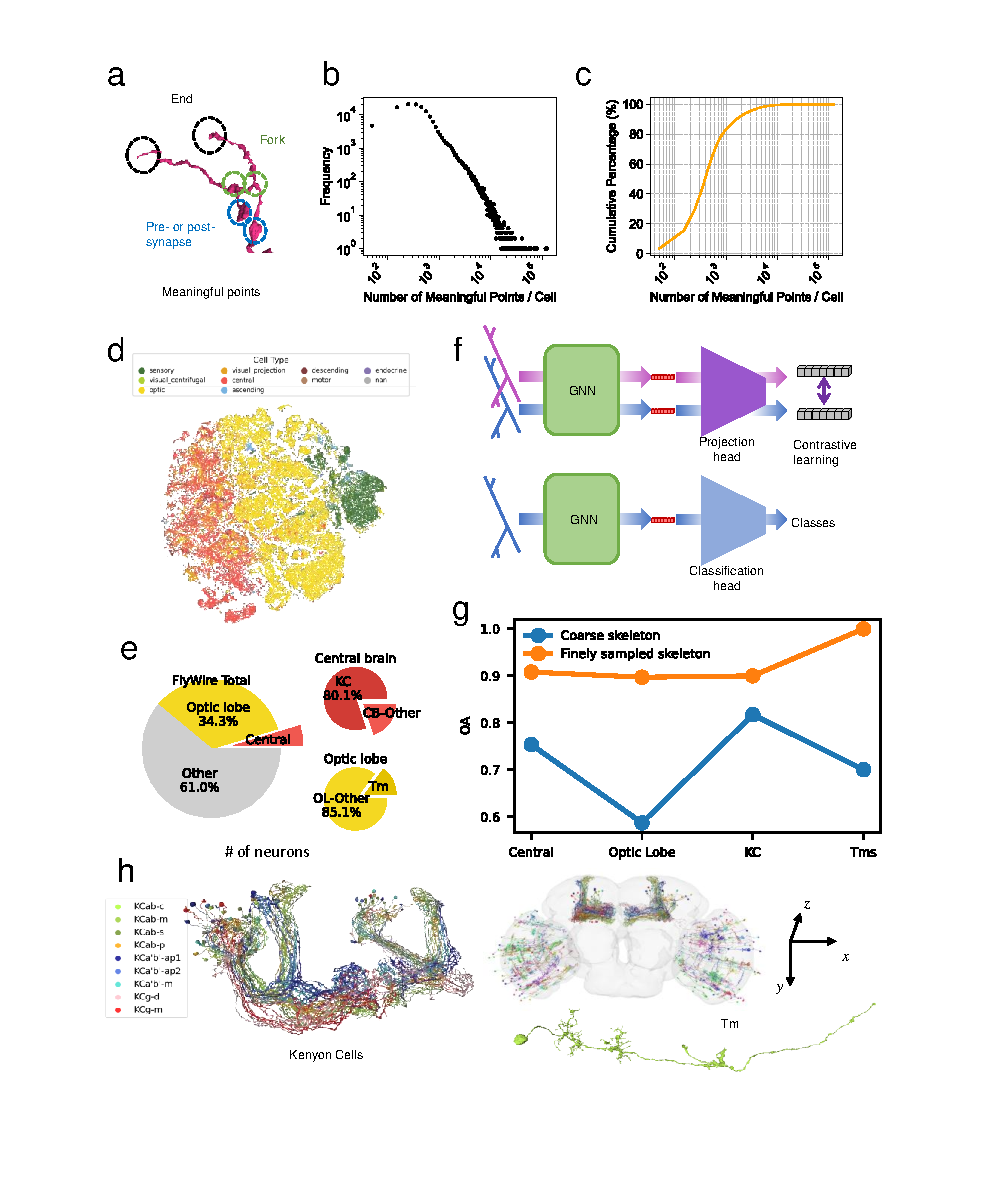
\includegraphics[width=1\linewidth]{figures/Fig1_0202.pdf}    
\caption{Finely sampled skeletons capture richer information for classification. \textbf{a},~Example neuron with end, fork, pre-/post-synapse labels. \textbf{b},~Distribution of meaningful node counts. \textbf{c},~Cumulative percentage. \textbf{d},~t-SNE of morphology representations colored by super class. \textbf{e},~Target neuron groups. \textbf{f},~Classification schematic. \textbf{g},~Accuracy comparison between coarse and fine skeletons. \textbf{h},~Example KC and Tm morphologies.}
\label{fig:morph_classify}
\end{figure}

% ── Result 2: Morphology sensitivity ───────────────────────────────────
\subsection*{Morphology representation is sensitive to nonfunctional features and spatial symmetry}

It is worth noting that contrastive learning is an unsupervised method for deriving features from large datasets. Thus, under the assumption of having no cell type labels, one may ask whether the latent representations can be exploited to analyze the commonalities and differences among neurons. Starting from this perspective, we performed t-SNE dimensionality reduction on the latent representations output by the GNN for FlyWire neuron skeletons. To visualize the latent distribution of different neuronal categories, neurons of different types were represented using different colours (Fig.~\ref{fig:morph_classify}d shows the distribution of different super classes across all FlyWire neurons; Fig.~\ref{fig:morph_sensitivity}a shows the distribution of different types among all KC neurons; Fig.~\ref{fig:morph_sensitivity}h shows the distribution of different Tm types).

The distribution of KC types exhibits multiple clusters (Fig.~\ref{fig:morph_sensitivity}b). These clusters correspond to KC cell types, different hemilineages, and left-right brain hemispheres. KC neurons display pronounced morphological differences in their dendritic segments due to distinct developmental lineages (Fig.~\ref{fig:morph_sensitivity}c), and these differences are independent of KC classification types. By removing dendritic segments from the network input without retraining, we can eliminate the effects of developmental lineage (Fig.~\ref{fig:morph_sensitivity}d), revealing only left-right hemispheric and KC cell type differences. Clustering the morphological representations without dendritic segments yields the primary classification clusters within KC types; under this five-type clustering scheme, the correspondence between clustering types and original label types is shown in the pie chart in Fig.~\ref{fig:morph_sensitivity}f. Furthermore, by examining neurons of other types that fall within single-type clusters in Fig.~\ref{fig:morph_sensitivity}d, we identified instances of mislabeling. Fig.~\ref{fig:morph_sensitivity}e shows a KC$\alpha'\beta'$ neuron that was incorrectly classified as KC$\gamma$-m in the type labels---a finding that foreshadows the corrected KC type annotations used throughout the lateralization analysis below.

The t-SNE visualization of Tm neurons reveals a more dispersed distribution, with a Silhouette score of only 0.008. This fragmentation is partially attributable to the rotational and translational symmetries exhibited by optic lobe neurons, as well as the presence of non-functional segments arising from developmental processes. By computing the correlation between the y-coordinate of the soma and the latent representation of the cell, a significant association emerges, as visualized in Fig.~\ref{fig:morph_sensitivity}i. This spatial dependence means that neurons of the same type but at different positions in the optic lobe receive different morphological representations, undermining unsupervised clustering.

These findings indicate that non-functional segments arising from development and the spatial symmetry of neurons significantly impact morphological representations, posing fundamental challenges for unsupervised clustering. This motivates the development of coordinate-free topological representations that can disentangle structural identity from spatial confounds.

\begin{figure}[htbp]
\centering
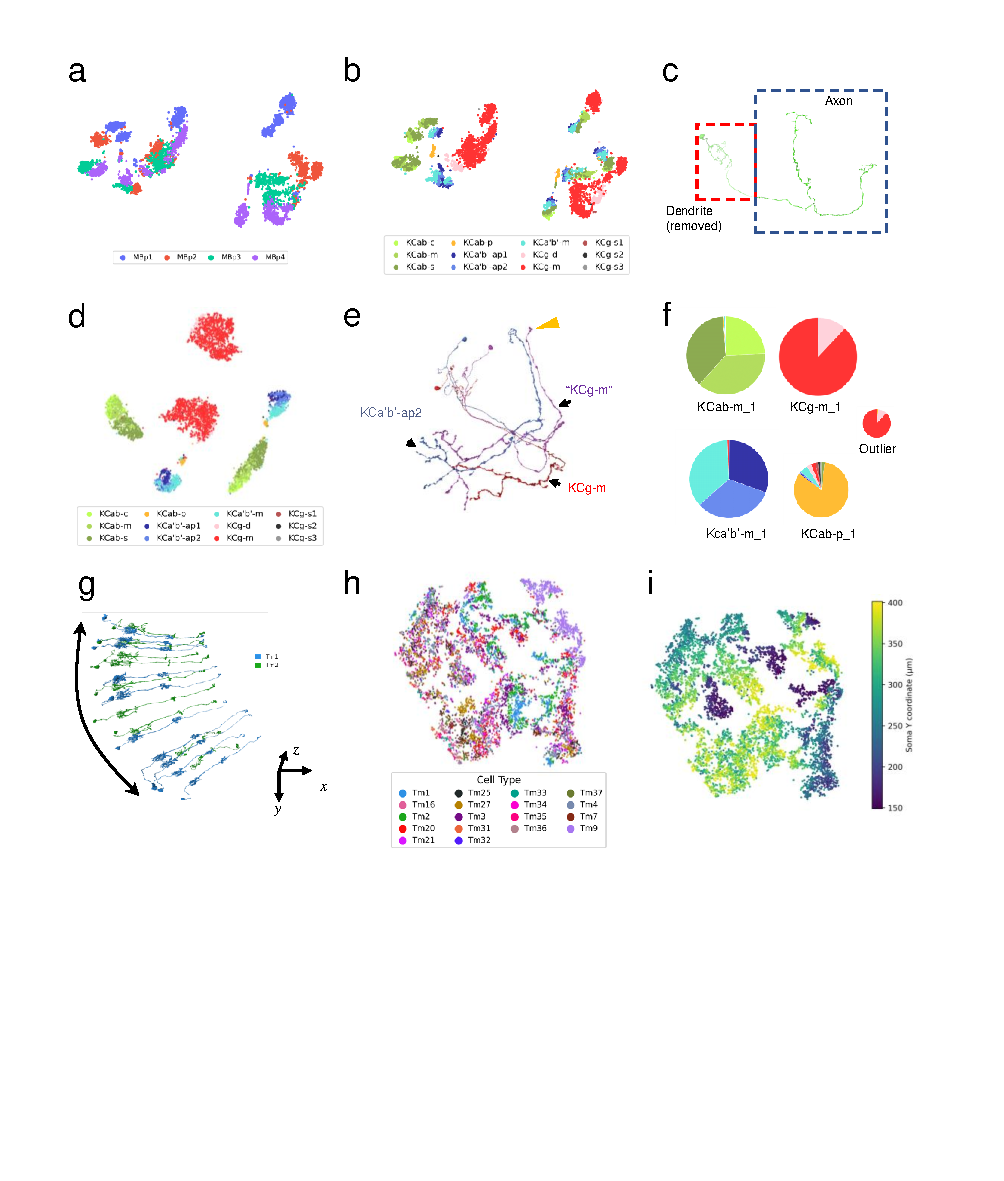
\includegraphics[width=1\linewidth]{figures/Fig2_0202.pdf}
\caption{Morphology representation is sensitive to nonfunctional features and spatial symmetry. \textbf{a,b},~t-SNE of KC morphology representations. \textbf{c},~Dendritic segment differences among hemilineages. \textbf{d},~t-SNE after removing dendritic segments. \textbf{e},~Mislabeled KC neuron. \textbf{f},~Cluster--type correspondence. \textbf{g},~Tm morphological variation along y-coordinate. \textbf{h},~Tm t-SNE. \textbf{i},~Soma y-coordinate correlation with latent representation.}
\label{fig:morph_sensitivity}
\end{figure}

% ── Result 3: Topology excels in clustering ────────────────────────────
\subsection*{Topology representation excels in clustering}

A portion of the sensitivity of morphological representations arises from their dependence on spatial coordinates. To disentangle this effect, we removed coordinate inputs while retaining the skeletal topological structure---the branching pattern, node degrees, and tree depth of the neuronal skeleton---which we refer to as the topological representation (Fig.~\ref{fig:topology}a). Compared with the morphological representation, the topological representation exhibits consistently improved intra-class compactness and inter-class separability across multiple evaluation settings, including all-neuron super classes, optic-lobe classes, Tm classes, and KC classes (Fig.~\ref{fig:topology}b--e, g--i).

Specifically, for KC neurons, the average inter-class distance increases from 5.639 (morphology) to 8.382 (topology), representing a 1.49-fold improvement in class separation, while the average intra-class distance decreases from 4.900 to 3.721, indicating 24.1\% tighter within-class clustering. The Silhouette score improves from $-0.048$ (morphology) to $0.090$ (topology). For Tm neurons, the inter-class distance increases from 12.077 to 12.692 (1.05-fold), while intra-class distance decreases from 9.445 to 6.696 (29.1\% reduction), with Silhouette scores of 0.008 and 0.210 respectively. Similar improvements are observed for neurons in CB (Silhouette scores: $-0.019$ vs 0.066) and OL ($-0.149$ vs 0.059). Together, these quantitative metrics demonstrate that the topological representation provides clear advantages over the morphological representation in unsupervised clustering, because the removal of spatial coordinates eliminates the confounding effects of hemispheric mirror symmetry, developmental lineage variation, and positional gradients.

These advantages are further reflected in few-label classification performance. We conducted classification experiments using only a small fraction of labelled data, selecting limited proportions of labels for CB, OL, KC, and Tm classification tasks. As shown in Fig.~\ref{fig:topology}f, in the five-class Kenyon cell classification task, reducing the labelled data ratio from 80\% to 10\% leads to a pronounced performance degradation in morphology-based representations (from 98\% to 85\%). By contrast, the accuracy of topology-based classification remains nearly unchanged and exceeds that of morphology-based classification at 10\% labelling, highlighting its improved robustness. This robustness is particularly important for practical applications where expert annotations are scarce.

The superior clustering properties of topology embeddings---which capture the essential structural identity of neurons while discarding confounding spatial variation---motivate their use as node features for downstream connectivity analysis. In the following sections, we leverage these 64-dimensional topology embeddings as the morphological component of a multi-modal feature vector, combining them with neurotransmitter-based connectivity features to identify how feature scale should be matched to circuit architecture in connectome feature engineering.

\begin{figure}[htbp]
\centering
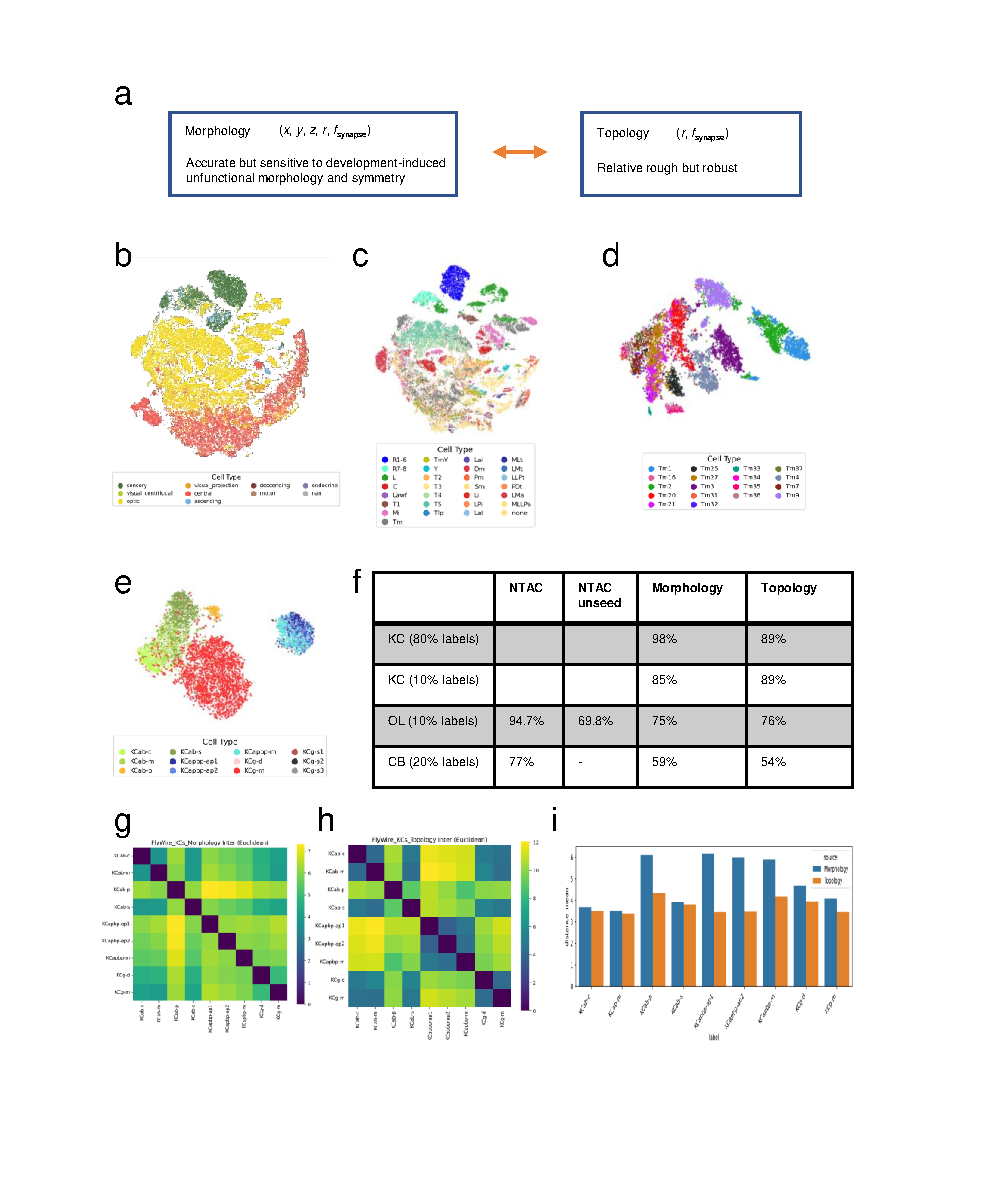
\includegraphics[width=1\linewidth]{figures/Fig3_0202.pdf}
\caption{Topology representation excels in clustering. \textbf{a},~Schematic of topology representation without coordinate inputs. \textbf{b--e},~t-SNE visualizations of topological representations for all neurons, optic lobe, Tm, and KC classes. \textbf{f},~Few-label classification accuracy comparison. \textbf{g--i},~Intra- and inter-class distance metrics.}
\label{fig:topology}
\end{figure}

% ── Result 4: Design principle ─────────────────────────────────────────
\subsection*{Circuit architecture determines optimal feature scale}

We defined NT Neighbor (10D; local partners within a population) and NT Circuit (10D; whole-brain partners) features and evaluated them with 5-nearest-neighbour classification (5-fold CV) across four neural populations (Fig.~\ref{fig:design}a, Table~\ref{tab:main}).

For KCs (9 types, $n=3{,}224$), NT Neighbor achieved 88.9\%, outperforming NT Circuit by +9.6\%. Central-brain neurons showed +7.0\%. Tm visual neurons showed the \textit{opposite}: NT Circuit outperformed by +20.1\%. This dissociation reveals a \textbf{feature-scale matching pattern}: the sign of $\Delta$ (local $-$ global) predicts whether a population is organized by modulatory input ($\Delta > 0$) or processing hierarchy ($\Delta < 0$; Fig.~\ref{fig:design}b).

The pattern replicated in the independent Hemibrain\cite{scheffer2020hemibrain} ($\Delta = +14.1\%$; Table~\ref{tab:cross}). MICrONS mouse V1\cite{microns2021cortical} showed $\Delta = +0.4\%$, consistent with more uniform cortical E/I organization. Multi-modal fusion (86D) improved most categories by +6.6\% to +14.1\% over topology alone (Fig.~\ref{fig:summary}a), with the two modalities capturing orthogonal information ($r < 0.3$). Notably, for KCs, fusion (80.2\%) performed \textit{below} NT Neighbor alone (88.9\%), because the fusion vector includes topology and NT Circuit, both of which are less informative for this population. This reinforces the same pattern: for modulatory circuits, adding global context can actively dilute the local signal.

\textbf{Graph neural network on the connectivity graph further supports this feature-scale matching pattern.} To test whether the topology--connectivity synergy extends beyond hand-crafted features, we trained a 3-layer Graph Attention Network (GAT) directly on the FlyWire connectivity graph (139,273 neurons as nodes, 2.5\,M synaptic connections as edges; Fig.~\ref{fig:gnn_workflow}). A systematic ablation study quantified the contribution of each modality (Table~\ref{tab:gnn}, Fig.~\ref{fig:ablation}):

\begin{itemize}
\item \textbf{Topology only} (64D node features + graph): 86.2\% accuracy (F1 = 0.82). The graph structure alone, propagating morphological embeddings through synaptic connections, provides a strong baseline.
\item \textbf{NT only} (5D node features + graph): 77.4\% (F1 = 0.69). With only 5 dimensions of NT prediction, the GNN still achieves respectable accuracy---far above the 40.7\% achieved by the same NT features \textit{without} graph structure (MLP baseline). This demonstrates that \textbf{graph message passing transforms sparse NT labels into informative neighbourhood signatures}, effectively recovering the hand-crafted NT Neighbor concept in a learned manner.
\item \textbf{Topology + NT} (69D + graph, full model): \textbf{88.3\%} accuracy (F1 = 0.86)---a +2.1\% gain over topology-only and +10.9\% over NT-only, confirming that the two modalities provide complementary information.
\item \textbf{Topology + NT, no graph} (69D, MLP): 83.7\% (F1 = 0.79). Removing graph structure costs $-$4.6\%, showing that synaptic connectivity provides information beyond what is encoded in per-neuron feature vectors.
\end{itemize}

The most striking result is the NT+graph synergy: NT features alone (5D MLP) achieve only 40.7\%, but when propagated through the connectivity graph, they reach 77.4\%---a +36.7 percentage point jump. This confirms that NT-based connectivity is fundamentally a \textit{relational} property: the informative signal lies not in a neuron's own NT identity, but in the NT composition of its synaptic neighbourhood, which the GNN captures through message passing. The asymmetry of this effect is biologically revealing: graph structure amplifies NT features by +36.7\% (from 40.7\% to 77.4\%) but topology features by only +4.6\% (from 83.7\% to 88.3\%), because the 64D topology embeddings already encode rich morphological information that is largely neuron-intrinsic, whereas the 5D NT labels are inherently relational---a KC$\gamma$-m and a KC$\alpha\beta$-c may have the same primary NT, but their \textit{neighbourhood NT distributions} are distinct. The GNN's message passing mechanism automatically recovers this local modulatory context, effectively learning the hand-crafted NT Neighbor concept in a data-driven manner.

The per-class analysis reveals that NT features disproportionately improve classification of minority types: macro-F1 increases from 0.82 to 0.86 (+3.9 percentage points), exceeding the accuracy gain (+2.1\%), indicating that NT connectivity is especially informative for types such as KC$\alpha\beta$-p ($n = 128$) and KC$\alpha'\beta'$-ap1 ($n = 280$) that are underrepresented in the training set. Detailed per-class results, including t-SNE visualization and confusion matrix, are shown in Fig.~\ref{fig:gnn_results}.

\begin{figure}[!ht]
\centering
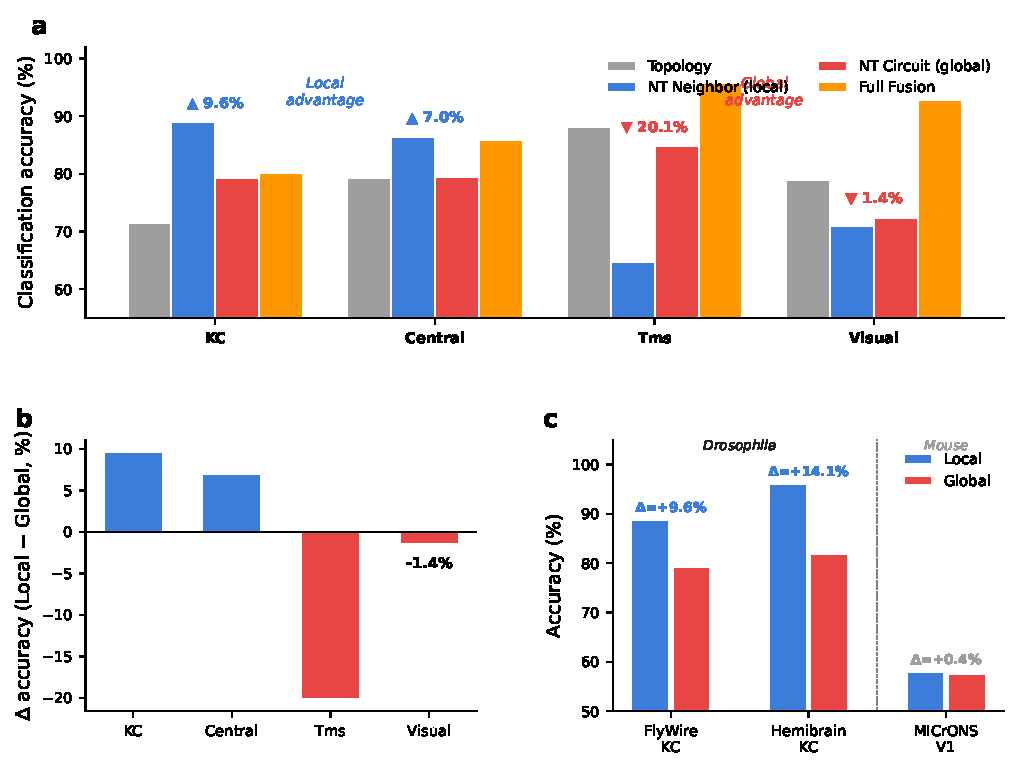
\includegraphics[width=\linewidth]{figures/Fig2_design_principle.pdf}
\caption{\textbf{Circuit architecture determines optimal feature scale.}
\textbf{a},~Classification accuracy for four feature types. Triangles: $\Delta$ (local $-$ global). KC and Central favour local; Tm and Visual favour global.
\textbf{b},~$\Delta$ waterfall.
\textbf{c},~Cross-dataset/species validation.}
\label{fig:design}
\end{figure}

\begin{table}[!ht]
\centering\small
\caption{\textbf{Classification accuracy (\%).} Bold: best single-modality. $\Delta$ = Neighbor $-$ Circuit.}
\label{tab:main}
\begin{tabular}{@{}lccccccc@{}}
\toprule
Category & $n$ & Classes & Topology & Neighbor & Circuit & $\Delta$ & Fusion \\
\midrule
KC       & 3,224 & 9  & 71.4 & \textbf{88.9} & 79.3 & \textcolor{blue!70!black}{+9.6}  & 80.2 \\
Central  & 2,768 & 12 & 79.3 & \textbf{86.4} & 79.4 & \textcolor{blue!70!black}{+7.0}  & 85.9 \\
\midrule
Tms      & 3,966 & 12 & 88.1 & 64.7 & \textbf{84.8} & \textcolor{red!70!black}{$-$20.1} & \textbf{95.7} \\
Visual   & 4,596 & 12 & 79.0 & 71.0 & 72.4 & \textcolor{red!70!black}{$-$1.4}  & \textbf{92.8} \\
\bottomrule
\end{tabular}
\end{table}

\begin{table}[!ht]
\centering\small
\caption{\textbf{Cross-dataset/species validation.}}
\label{tab:cross}
\begin{tabular}{@{}llcccc@{}}
\toprule
Dataset & Species & $n$ & Local & Global & $\Delta$ \\
\midrule
FlyWire KC    & \textit{Drosophila} & 3,224 & 88.9 & 79.3 & +9.6  \\
Hemibrain KC  & \textit{Drosophila} & 1,915 & \textbf{96.2} & 82.0 & +14.1 \\
MICrONS V1   & Mouse               & 8,000 & 58.0 & 57.6 & +0.4  \\
\bottomrule
\end{tabular}
\end{table}

\begin{figure}[!ht]
\centering
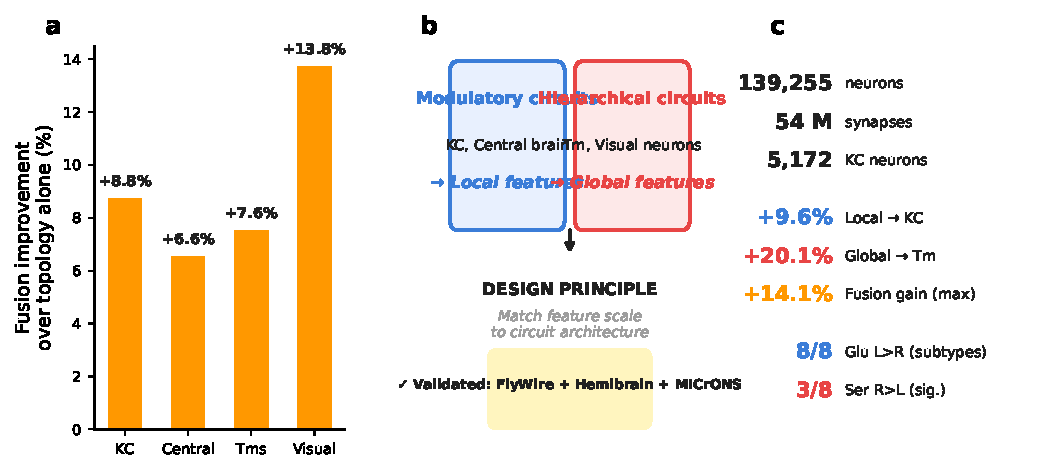
\includegraphics[width=\linewidth]{figures/Fig4_fusion_summary.pdf}
\caption{\textbf{Multi-modal fusion and feature-scale summary.}
\textbf{a},~Fusion improvement over topology alone for each category (+6.6\% to +14.1\%).
\textbf{b},~Feature-scale matching pattern: modulatory circuits (KC, Central) favour local features; hierarchical circuits (Tm, Visual) favour global features. Observed across FlyWire, Hemibrain, and MICrONS.
\textbf{c},~Key quantitative results.}
\label{fig:summary}
\end{figure}

\begin{figure}[!ht]
\centering
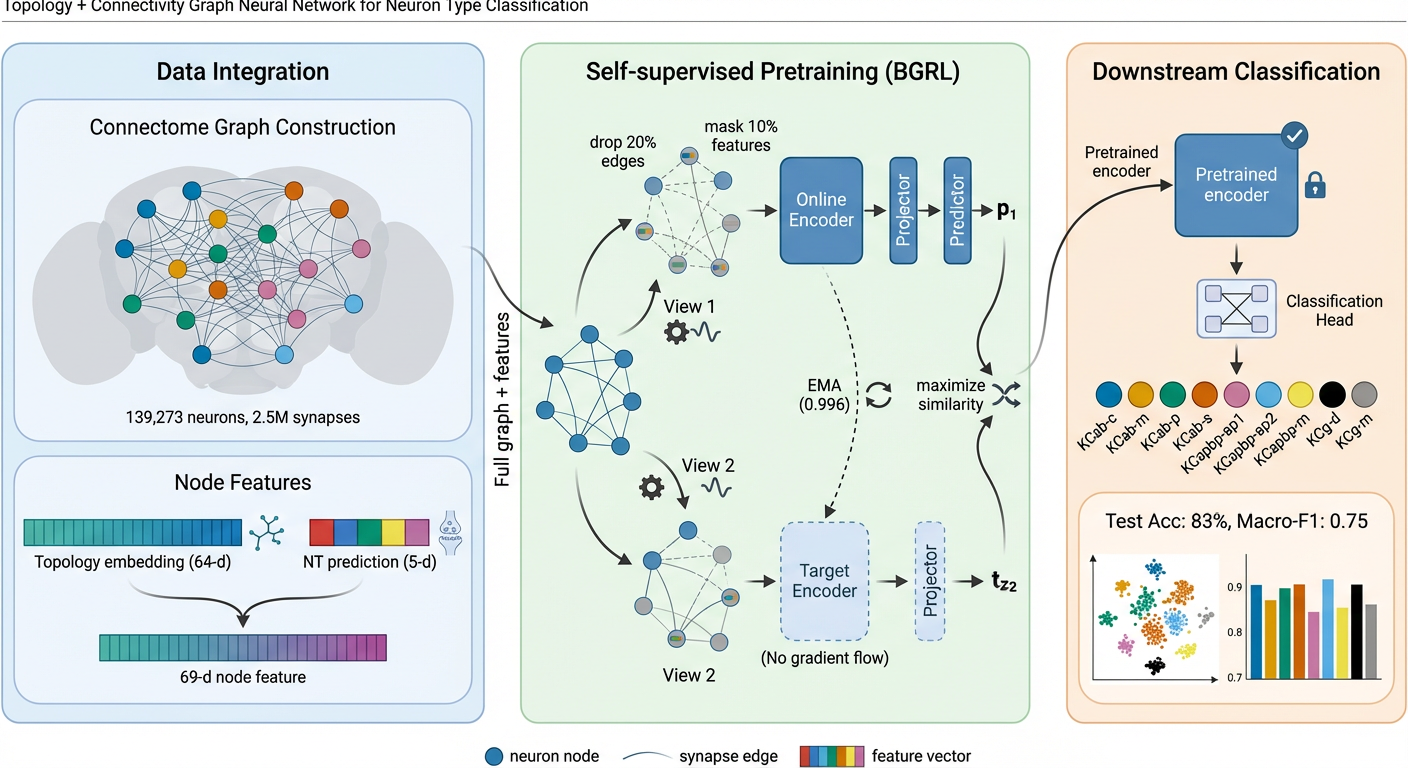
\includegraphics[width=\linewidth]{figures/Fig9_GNN_workflow.png}
\caption{\textbf{Connectivity-graph GNN supports the feature-scale matching pattern via graph-based learning.}
\textbf{Left}: The FlyWire connectome is represented as a graph (139,273 neuron nodes, 2.5\,M synaptic edges). Node features are the concatenation of 64D topology embedding and 5D NT prediction (69D total). \textbf{Centre}: Self-supervised pretraining with BGRL. \textbf{Right}: Classification head fine-tuned for 9 KC types (88.3\% accuracy, macro-F1 = 0.86).}
\label{fig:gnn_workflow}
\end{figure}

\begin{table}[!ht]
\centering\small
\caption{\textbf{KC classification: hand-crafted features vs.\ GNN ablation.}}
\label{tab:gnn}
\begin{tabular}{@{}llccc@{}}
\toprule
Method & Features & Graph & Acc (\%) & F1 \\
\midrule
\multicolumn{5}{@{}l}{\textit{Hand-crafted features (KNN classifier)}} \\
\quad Topology only   & 64D  & ---  & 71.4 & --- \\
\quad NT Circuit      & 10D  & ---  & 79.3 & --- \\
\quad Fusion          & 86D  & ---  & 80.2 & --- \\
\quad NT Neighbor     & 10D  & ---  & \textbf{88.9} & --- \\
\midrule
\multicolumn{5}{@{}l}{\textit{GNN on connectivity graph (ablation)}} \\
\quad NT only (MLP)   & 5D   & \texttimes  & 40.7 & 0.06 \\
\quad NT only + GNN   & 5D   & \checkmark  & 77.4 & 0.69 \\
\quad Topo only + GNN & 64D  & \checkmark  & 86.2 & 0.82 \\
\quad Topo+NT (MLP)   & 69D  & \texttimes  & 83.7 & 0.79 \\
\quad \textbf{Topo+NT + GNN}  & \textbf{69D}  & \checkmark  & \textbf{88.3} & \textbf{0.86} \\
\bottomrule
\end{tabular}
\end{table}

\begin{figure}[!ht]
\centering
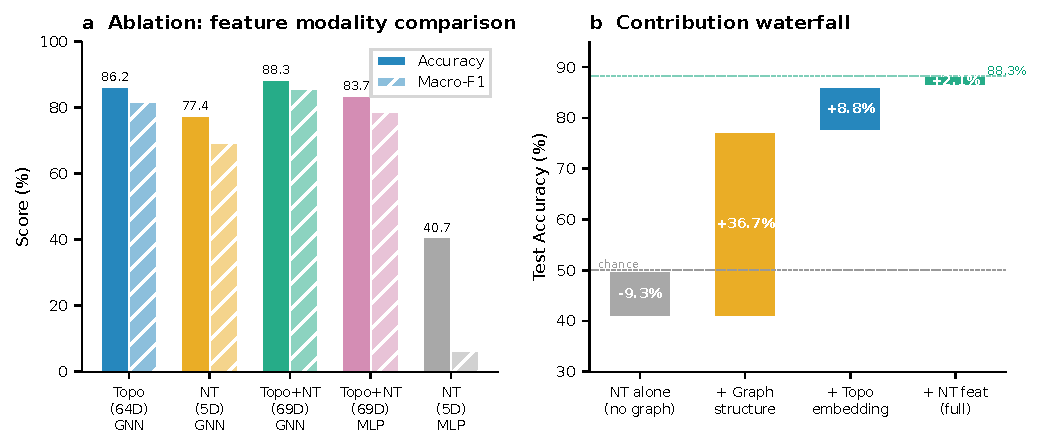
\includegraphics[width=\linewidth]{figures/Fig11_ablation.pdf}
\caption{\textbf{GNN ablation study.}
\textbf{a},~Accuracy and macro-F1 for five conditions.
\textbf{b},~Contribution waterfall showing how each component adds to classification accuracy.}
\label{fig:ablation}
\end{figure}

% ── Result 5: Lateralization ───────────────────────────────────────────
\subsection*{Pervasive lateralization of neuromodulatory input to Kenyon Cells}

To test whether NT input profiles encode laterality, we compared left ($n=2{,}577$) and right ($n=2{,}595$) KC neurons directly (Mann--Whitney $U$, 45 tests with both Bonferroni and Benjamini--Hochberg FDR correction; Fig.~\ref{fig:hemi}, Table~\ref{tab:asym}). Critically, we used corrected KC type annotations that properly distinguish the $\alpha'\beta'$ lobe (prefix KCapbp-) from $\alpha\beta$ (prefix KCab-), resolving a previously unreported conflation: 338 neurons belonging to KC$\alpha'\beta'$-m were misassigned to KC$\alpha\beta$-m in the original \texttt{hemibrain\_type} field of the FlyWire classification, yielding 9 types rather than 8.

\textbf{The asymmetry is pervasive but graded by lobe system.} Of 45 type$\times$NT tests, 27 were significant after Bonferroni correction and 36 after FDR correction. All 9 KC types showed at least one significant NT difference (Fig.~\ref{fig:deep}a, Table~\ref{tab:asym}). The three $\alpha'\beta'$ types exhibited the largest effects: KC$\alpha'\beta'$-ap2 showed the strongest glutamate left-bias ($d = -1.47$, Cliff's $\delta = 0.72$, $p_\mathrm{Bonf} = 4.1 \times 10^{-25}$) and serotonin right-enrichment ($d = +1.45$, $p_\mathrm{Bonf} = 6.6 \times 10^{-25}$). KC$\alpha'\beta'$-ap1 showed concordant patterns (Ser $d = +1.34$, GABA $d = -1.11$, Glu $d = -0.90$). The newly resolved KC$\alpha'\beta'$-m ($n = 338$; L~164, R~174) showed effects indistinguishable from the other $\alpha'\beta'$ types (Ser $d = +1.35$, $p_\mathrm{Bonf} = 1.9 \times 10^{-27}$; Glu $d = -1.47$; GABA $d = -1.04$), confirming it as a bona fide $\alpha'\beta'$ population. Even the $\gamma$ lobe types showed significant serotonin right-enrichment: KC$\gamma$-m ($d = +0.56$, $p_\mathrm{Bonf} = 9.5 \times 10^{-48}$) and KC$\gamma$-d ($d = +0.66$, $p_\mathrm{Bonf} = 1.3 \times 10^{-5}$).

\textbf{Serotonin right-enrichment is the most consistent cross-type signal.} Serotonergic input was right-enriched in all 9/9 types (binomial $p = 0.004$), with 7 individually significant after Bonferroni correction (Table~\ref{tab:asym}). Cliff's delta confirmed large effects ($|\delta| > 0.70$) for the $\alpha'\beta'$ types and medium effects ($|\delta| = 0.24$--$0.37$) for $\gamma$ types. Split-half reliability analysis showed 100\% sign consistency across 100 random half-splits for all types with $|d| > 0.3$.

\textbf{Glutamate left-bias is the second most consistent signal.} Left-hemisphere KCs received more glutamatergic input in 7/9 types, with 7 individually significant after Bonferroni correction ($d = -0.27$ to $-1.47$).

\textbf{Dopamine right-enrichment parallels serotonin.} Extending the analysis to all six predicted neurotransmitters (54 tests = 9 types $\times$ 6 NTs), we found that dopaminergic input was right-enriched in 6/9 types, with 5 individually significant (max $|d| = 1.42$ for KC$\alpha'\beta'$-ap2). The $\alpha'\beta'$ types showed extreme DA right-enrichment ($d = +1.34$ to $+1.42$) with the same directionality as serotonin, consistent with a coordinated neuromodulatory gradient. GABA showed left-enrichment in 5/9 types (6 significant; max $|d| = 1.26$), and octopamine showed mixed lateralization (6 significant; max $|d| = 0.56$). Across all 54 tests, 32 were Bonferroni-significant and 44 FDR-significant (Extended Data Fig.~\ref{fig:ext_heatmap}).

\textbf{Multi-classifier validation confirms hemisphere separability.} Four independent classifiers (KNN, Random Forest, SVM, Logistic Regression) trained to predict hemisphere from the 5D NT input profile all exceeded chance across all 9 types (Fig.~\ref{fig:validation}a). The $\alpha'\beta'$ types achieved 86--88\% accuracy, while $\gamma$-m achieved 60--68\%.

\textbf{Independent secondary validation with multiple orthogonal methods.} We validated the lateralization findings using seven complementary statistical approaches applied to all six NTs (Extended Data Fig.~\ref{fig:ext_heatmap}--\ref{fig:ext_convergence}). (i)~GPU-accelerated permutation tests (10,000 label shuffles per test) confirmed 30/54 significant effects after Bonferroni correction, with serotonin significant in 7/9 types (Extended Data Fig.~\ref{fig:ext_perm}). (ii)~Bootstrap bias-corrected accelerated (BCa) 95\% confidence intervals (10,000 resamples) excluded zero for 41/54 tests; serotonin CIs excluded zero in all 9/9 types (Extended Data Fig.~\ref{fig:ext_forest}). (iii)~Bayesian $t$-tests (JZS prior, integral-based BF$_{10}$; Rouder et al.\ 2009) yielded extreme evidence (BF$_{10} > 100$) for 25/54 tests, with serotonin showing extreme evidence in 7/9 types (Extended Data Fig.~\ref{fig:ext_bayes}). (iv)~SIMEX measurement-error extrapolation confirmed that all serotonin effects maintained their direction when extrapolated to zero measurement error (9/9 R$>$L preserved; Extended Data Fig.~\ref{fig:ext_simex}). (v)~Gold's iterative deconvolution of the Eckstein et al.\ confusion matrix yielded 30/54 significant effects, with 100\% direction preservation for effects with $|d| > 0.3$ (Extended Data Fig.~\ref{fig:ext_deconv}). (vi)~Hotelling's $T^2$ multivariate test on the full 6D NT profile confirmed significant hemispheric differences in all 9/9 types (all $p < 10^{-13}$ after Bonferroni correction). (vii)~Volcano plot analysis across all 54 tests revealed a striking asymmetry: serotonin and dopamine cluster in the R$>$L quadrant while glutamate and GABA cluster in L$>$R, confirming coordinated neuromodulatory lateralization (Extended Data Fig.~\ref{fig:ext_volcano}). The convergence of these seven methods provides strong evidence against statistical artifacts (Extended Data Fig.~\ref{fig:ext_convergence}).

\textbf{Upstream neuron identity reveals a cell-class imbalance.} To determine whether the NT asymmetry reflects differences in upstream \textit{cell-type composition}, we identified synapses with serotonin-dominant NT predictions ($\mathrm{ser\_avg} > 0.5$) to KC$\alpha'\beta'$-ap1 and KC$\alpha'\beta'$-m and classified the presynaptic neurons by FlyWire cell class. For both types, right-hemisphere KCs received 57 serotonin-predicted synapses from DANs versus 6 in the left---a 9.5-fold enrichment (Fisher's exact test, $p = 2.2 \times 10^{-5}$ for ap1; $p = 3.5 \times 10^{-7}$ for KC$\alpha'\beta'$-m; Fig.~\ref{fig:upstream}a). This imbalance was robust across serotonin thresholds (confirmed at 0.3 and 0.7) and was also significant for KC$\gamma$-d (7.8$\times$, $p = 7.8 \times 10^{-7}$), KC$\gamma$-m (4.8$\times$, $p = 1.2 \times 10^{-19}$), and KC$\alpha\beta$-s (3.9$\times$, $p = 2.5 \times 10^{-9}$). Left-hemisphere KCs received proportionally more input from MBINs.

\textbf{A note on DAN--serotonin co-occurrence.} The finding that synapses classified as serotonin-dominant originate from neurons annotated as dopaminergic (DAN) merits caution. This could reflect (i)~limitations of the per-synapse NT classifier, which has lower accuracy for serotonin ($\sim$80\%) than for ACh or GABA ($>$90\%)\cite{eckstein2020neurotransmitter}; (ii)~genuine co-transmission, as some DANs are known to co-release neuropeptides alongside dopamine; or (iii)~cell-class annotation granularity in FlyWire, where `DPM'-type neurons---the principal serotonergic modulators of $\alpha'\beta'$ KCs\cite{keene2006dpm}---may not carry an explicit DPM cell-type label. We did not find neurons labelled ``DPM'' in the FlyWire cell-type annotations, suggesting they may be classified under a broader MBIN or DAN category. The key finding---that the upstream cell-class composition differs between hemispheres---is independent of how the NT prediction is interpreted.

\textbf{Input synapse counts are balanced; asymmetry is in NT composition.} Despite the NT differences, total input synapse counts were highly correlated between hemispheres ($r = 0.996$; Fig.~\ref{fig:deep}c), and ipsilateral input fraction was $>$90\% for all types (Fig.~\ref{fig:deep}d). The asymmetry is therefore not a wiring artifact but a genuine difference in the \textit{neurotransmitter identity} of presynaptic partners. Note that KC--KC connections are 100\% cholinergic and carry no NT variance; the lateralization arises entirely from non-KC inputs. The lobe-system analysis (Fig.~\ref{fig:upstream}d) confirms that $\alpha'\beta'$ drives the strongest effect, with a graded decrease through $\alpha\beta$ to $\gamma$---mapping onto the memory-consolidation hierarchy (Fig.~\ref{fig:lobe_memory}).

\begin{figure}[!ht]
\centering
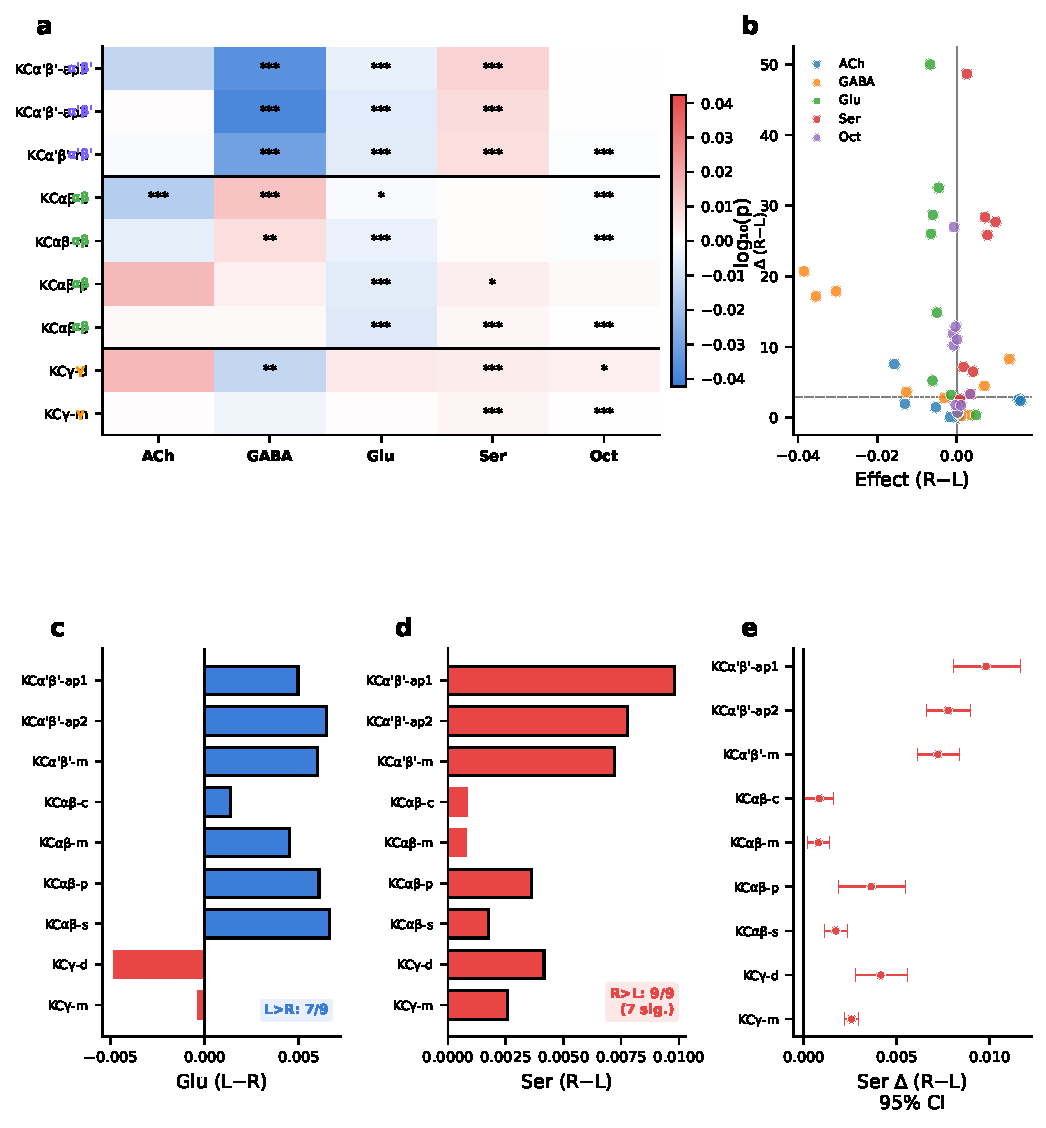
\includegraphics[width=\linewidth]{figures/Fig3_hemisphere_asymmetry.pdf}
\caption{\textbf{Lobe-specific hemispheric NT input asymmetry in Kenyon Cells (corrected labels).}
\textbf{a},~Effect-size heatmap (R $-$ L) for all 9 types.
\textbf{b},~Volcano plot.
\textbf{c},~Glutamate L-bias (7/9).
\textbf{d},~Serotonin R-enrichment (9/9).
\textbf{e},~Bootstrap BCa 95\% CIs.}
\label{fig:hemi}
\end{figure}

\begin{figure}[!ht]
\centering
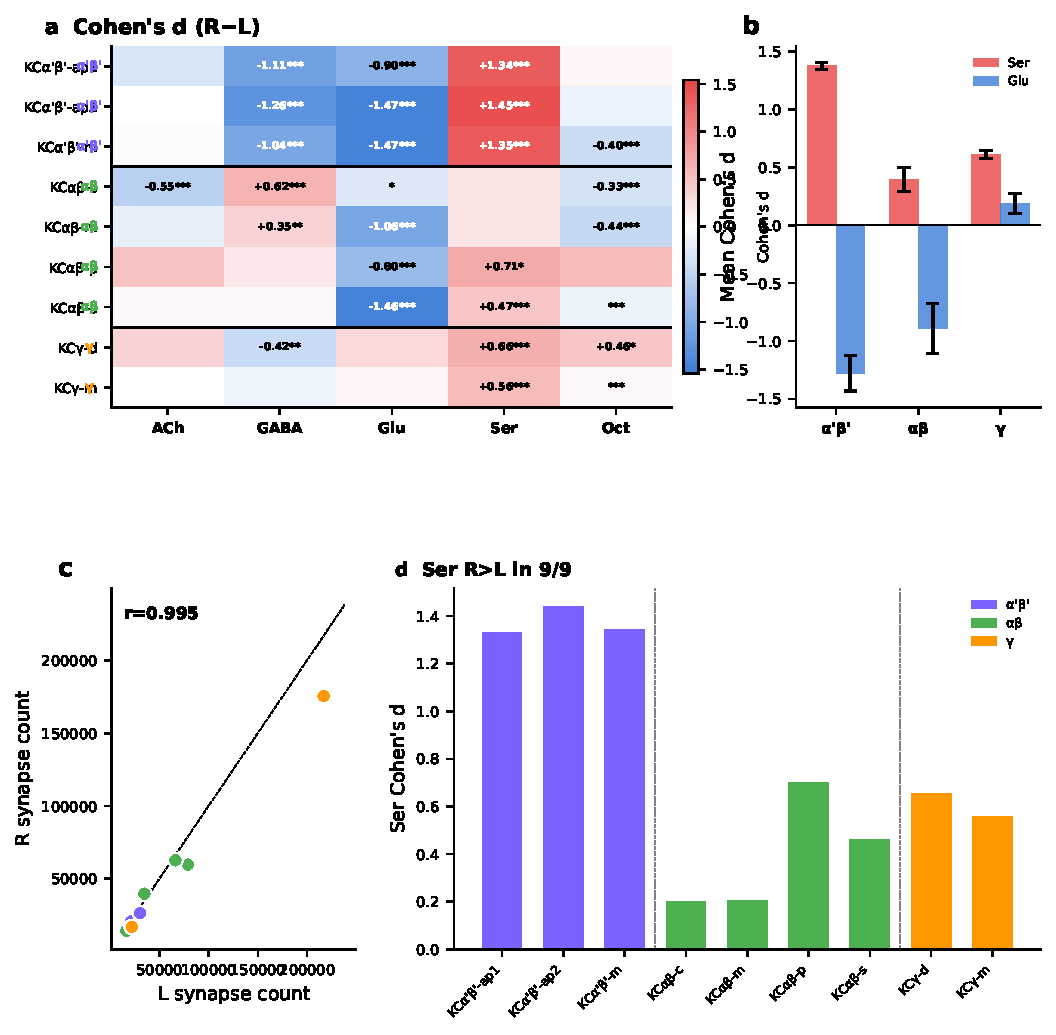
\includegraphics[width=\linewidth]{figures/Fig5_deep_asymmetry.pdf}
\caption{\textbf{Deep analysis of KC hemispheric asymmetry (all 9 types, corrected labels).}
\textbf{a},~Cohen's $d$ heatmap with lobe-system annotation.
\textbf{b},~Lobe-system grouped effect sizes.
\textbf{c},~Balanced input synapse counts ($r = 0.996$).
\textbf{d},~Ipsilateral input fraction.
\textbf{e},~Serotonin R$>$L in 9/9 types.}
\label{fig:deep}
\end{figure}

\begin{table}[!ht]
\centering\small
\caption{\textbf{Hemispheric NT input asymmetry} (Mann--Whitney $U$, Bonferroni-corrected, 54 tests). $d$: Cohen's $d$. Serotonin R$>$L in 9/9 types (binomial $p = 0.004$); DA R$>$L in 6/9.}
\label{tab:asym}
\begin{tabular}{@{}lccccccc@{}}
\toprule
KC type & Lobe & ACh & GABA & Glu & Ser & Oct & DA \\
\midrule
KC$\alpha'\beta'$-ap1 & $\alpha'\beta'$ & --- & L$^{\ast\ast\ast}$ ($d{=}{-}1.11$) & L$^{\ast\ast\ast}$ ($d{=}{-}0.90$) & R$^{\ast\ast\ast}$ ($d{=}{+}1.34$) & --- & R$^{\ast\ast\ast}$ ($d{=}{+}1.34$) \\
KC$\alpha'\beta'$-ap2 & $\alpha'\beta'$ & --- & L$^{\ast\ast\ast}$ ($d{=}{-}1.26$) & L$^{\ast\ast\ast}$ ($d{=}{-}1.47$) & R$^{\ast\ast\ast}$ ($d{=}{+}1.45$) & --- & R$^{\ast\ast\ast}$ ($d{=}{+}1.42$) \\
KC$\alpha'\beta'$-m   & $\alpha'\beta'$ & --- & L$^{\ast\ast\ast}$ ($d{=}{-}1.04$) & L$^{\ast\ast\ast}$ ($d{=}{-}1.47$) & R$^{\ast\ast\ast}$ ($d{=}{+}1.35$) & L$^{\ast\ast\ast}$ & R$^{\ast\ast\ast}$ ($d{=}{+}1.38$) \\
\midrule
KC$\alpha\beta$-c     & $\alpha\beta$   & L$^{\ast\ast\ast}$ & R$^{\ast\ast\ast}$ & L$^{\ast}$ ($d{=}{-}0.27$) & --- & L$^{\ast\ast\ast}$ & --- \\
KC$\alpha\beta$-m     & $\alpha\beta$   & --- & R$^{\ast\ast}$ & L$^{\ast\ast\ast}$ ($d{=}{-}1.06$) & --- & L$^{\ast\ast\ast}$ & R$^{\ast\ast\ast}$ \\
KC$\alpha\beta$-p     & $\alpha\beta$   & --- & --- & L$^{\ast\ast\ast}$ ($d{=}{-}0.80$) & R$^{\ast}$ ($d{=}{+}0.71$) & --- & --- \\
KC$\alpha\beta$-s     & $\alpha\beta$   & --- & --- & L$^{\ast\ast\ast}$ ($d{=}{-}1.46$) & R$^{\ast\ast\ast}$ ($d{=}{+}0.47$) & L$^{\ast\ast\ast}$ & R$^{\ast\ast}$ \\
\midrule
KC$\gamma$-d          & $\gamma$        & --- & L$^{\ast\ast}$ & --- & R$^{\ast\ast\ast}$ ($d{=}{+}0.66$) & R$^{\ast}$ & --- \\
KC$\gamma$-m          & $\gamma$        & --- & --- & --- & R$^{\ast\ast\ast}$ ($d{=}{+}0.56$) & R$^{\ast\ast\ast}$ & --- \\
\midrule
\multicolumn{8}{@{}l@{}}{\textit{Ser consensus: R $>$ L in 9/9 types (binomial $p = 0.004$); 7/9 Bonferroni-significant}} \\
\multicolumn{8}{@{}l@{}}{\textit{Glu consensus: L $>$ R in 7/9 types; 7 Bonferroni-significant ($d = -0.27$ to $-1.47$)}} \\
\multicolumn{8}{@{}l@{}}{\textit{DA consensus: R $>$ L in 6/9 types; 5 Bonferroni-significant (max $d = +1.42$)}} \\
\multicolumn{8}{@{}l@{}}{\textit{Total: 32/54 Bonferroni-significant; 44/54 FDR-significant}} \\
\bottomrule
\end{tabular}
\end{table}

\begin{figure}[!ht]
\centering
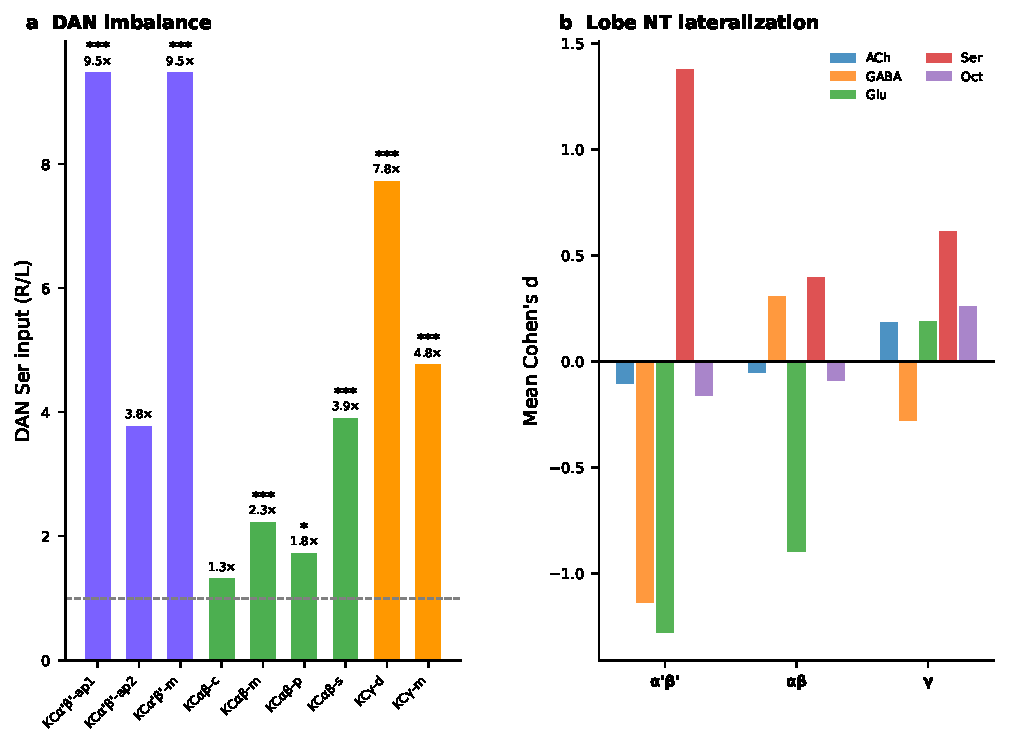
\includegraphics[width=\linewidth]{figures/Fig6_upstream_decomposition.pdf}
\caption{\textbf{Upstream cell-type decomposition of the serotonin asymmetry.}
\textbf{a},~Serotonergic synapses classified by upstream cell class. 9.5$\times$ DAN enrichment in the right hemisphere.
\textbf{b},~DAN serotonergic input ratio (R/L) across all 9 types.
\textbf{c},~Full NT profile of non-KC inputs.
\textbf{d},~Lobe-system grouped Cohen's $d$.}
\label{fig:upstream}
\end{figure}

\begin{figure*}[!ht]
\centering
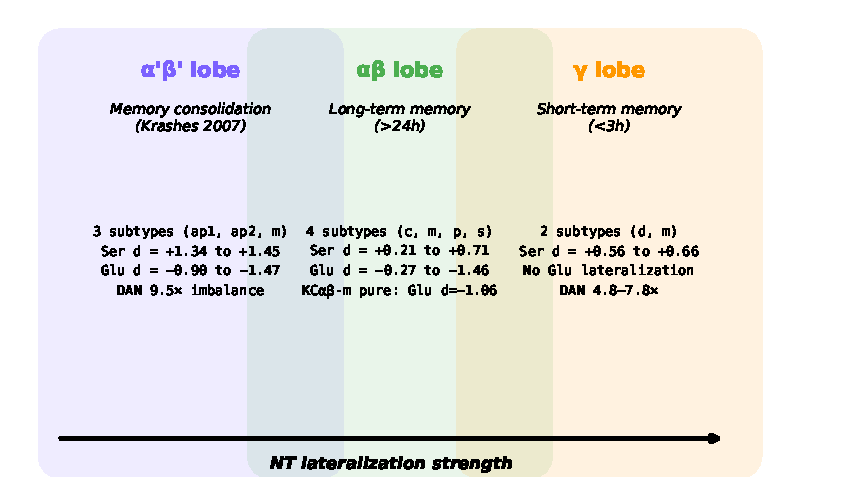
\includegraphics[width=0.95\linewidth]{figures/Fig7_lobe_memory_schematic.pdf}
\caption{\textbf{Lobe-specific lateralization maps onto memory-function divisions.}
The $\alpha'\beta'$ lobe (3 types, $n = 916$), required for memory consolidation, shows the strongest NT lateralization (Ser $d = +1.34$ to $+1.45$; Glu $d = -0.90$ to $-1.47$). The $\alpha\beta$ lobe shows intermediate asymmetry. The $\gamma$ lobe shows moderate serotonin asymmetry but no glutamate effects.}
\label{fig:lobe_memory}
\end{figure*}

\begin{figure}[!ht]
\centering
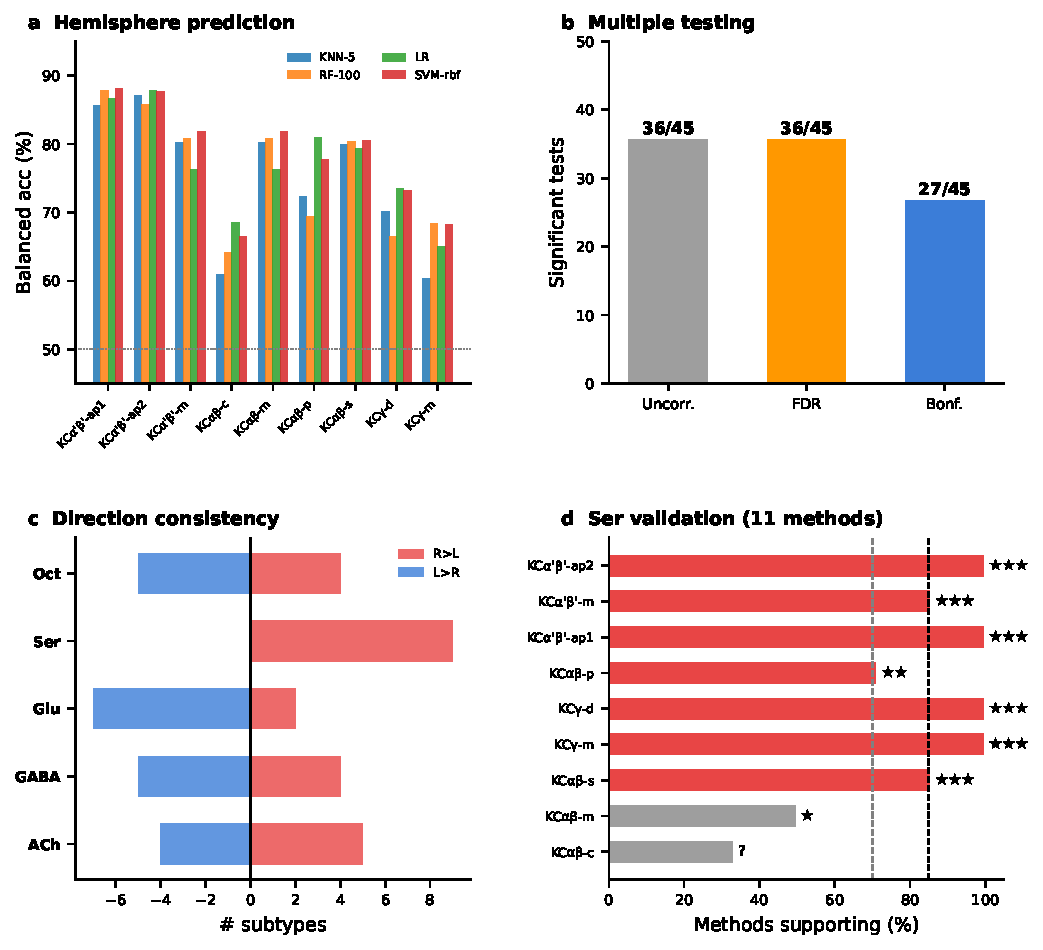
\includegraphics[width=\linewidth]{figures/Fig8_enhanced_validation.pdf}
\caption{\textbf{Multi-method validation of hemispheric NT asymmetry.}
\textbf{a},~Hemisphere prediction using four classifiers.
\textbf{b},~Multiple testing correction comparison.
\textbf{c},~Cross-type NT direction consistency.
\textbf{d},~11-method secondary validation convergence.}
\label{fig:validation}
\end{figure}

% ── Result 6: Additional biological analyses ──────────────────────────
\subsection*{Lateralization is lobe-graded, input-specific, and extends beyond the mushroom body}

To further characterize the lateralization, we performed three additional analyses.

\textbf{Lobe-level (compartment) analysis confirms the graded pattern.} When KC neurons are pooled by lobe system rather than type, the lateralization gradient is preserved and strengthened by increased statistical power (Table~\ref{tab:lobe}). The $\alpha'\beta'$ lobe shows the strongest serotonin right-enrichment ($d = +1.33$, $p < 10^{-78}$) and glutamate left-bias ($d = -1.24$, $p < 10^{-68}$). The $\alpha\beta$ lobe shows intermediate effects (Ser $d = +0.30$; Glu $d = -0.81$). The $\gamma$ lobe shows significant serotonin asymmetry ($d = +0.56$, $p < 10^{-52}$) but no glutamate lateralization ($d = +0.11$, n.s.). At the whole-MB level, serotonin ($d = +0.58$, $p < 10^{-90}$) and glutamate ($d = -0.33$, $p < 10^{-69}$) are both highly significant. Of 15 lobe$\times$NT tests, 11 are Bonferroni-significant. This compartment-level analysis confirms that the lateralization follows a functional gradient aligned with memory processing: the $\alpha'\beta'$ lobe (memory consolidation) is most lateralized, the $\gamma$ lobe (short-term memory) is least, and the $\alpha\beta$ lobe (long-term memory) is intermediate.

\begin{table}[!ht]
\centering\small
\caption{\textbf{Lobe-level lateralization.} Cohen's $d$ (R $-$ L convention) for each lobe system and whole MB. Bonferroni-corrected over 15 tests (lobe) or 5 tests (whole MB). 11/15 lobe-level and 4/5 whole-MB tests are significant.}
\label{tab:lobe}
\begin{tabular}{@{}lcccccc@{}}
\toprule
Lobe & $n_\mathrm{L}$ & $n_\mathrm{R}$ & ACh & GABA & Glu & Ser \\
\midrule
$\alpha'\beta'$ & 450 & 466 & $-$0.09 & $-$1.13$^{\ast\ast\ast}$ & $-$1.24$^{\ast\ast\ast}$ & $+$1.33$^{\ast\ast\ast}$ \\
$\alpha\beta$   & 911 & 860 & $-$0.09 & $+$0.30$^{\ast\ast\ast}$ & $-$0.81$^{\ast\ast\ast}$ & $+$0.30$^{\ast\ast\ast}$ \\
$\gamma$        & 1,216 & 1,269 & $+$0.07 & $-$0.17$^{\ast\ast\ast}$ & $+$0.11 & $+$0.56$^{\ast\ast\ast}$ \\
\midrule
All KC          & 2,577 & 2,595 & $-$0.03 & $-$0.18$^{\ast\ast}$ & $-$0.33$^{\ast\ast\ast}$ & $+$0.58$^{\ast\ast\ast}$ \\
\bottomrule
\end{tabular}
\end{table}

\textbf{The lateralization is input-specific: KC outputs are uniformly cholinergic.} We examined whether the NT asymmetry extends to KC output synapses. Analysis of 563,235 output connections from KCs revealed that all KC output synapses are 100\% cholinergic (ACh = 1.0, all other NTs = 0.0) with zero variance across all neurons and types. Output-side NT lateralization is therefore not applicable. This confirms that the lateralization is exclusively in the NT composition of \textit{inputs} to KCs---what they receive from upstream partners---not in their own neurotransmitter output. KCs are a homogeneous cholinergic population whose functional diversity arises from differential upstream modulation.

\textbf{Serotonin right-enrichment extends to central-brain neurons.} To test whether the lateralization is specific to KCs, we performed the same analysis on central-brain and visual neuron populations using corrected type labels. Central-brain neurons (7 types with $\geq$50 neurons per hemisphere) showed serotonin right-enrichment in 7/7 types, with 20/35 tests Bonferroni-significant (mean $|d| = 0.58$, max $|d| = 1.47$). This pattern closely mirrors the KC findings, suggesting that the serotonin hemispheric gradient extends beyond the mushroom body to the broader central brain. By contrast, visual neurons (1 testable type) showed a different pattern (Ser L$>$R), consistent with the distinct circuit architecture of the optic lobe. Tm neurons had insufficient per-type sample sizes for hemisphere-stratified analysis. The finding that central-brain neurons share the serotonin lateralization pattern with KCs argues against a KC-specific mechanism and instead favours a brain-wide developmental program that establishes hemispheric serotonergic gradients.

\subsection*{Connectome-constrained simulations link lateralized circuits to food-odour memory}

The NT lateralization results above identify hemispheric differences in the transmitter composition of KC inputs, but do not by themselves specify how these differences could influence behaviour. We therefore asked whether the same FlyWire v783 connectivity table supports a circuit-level mechanism that can be projected into an embodied behavioural assay. We directly mined the proofread neuron-to-neuron connection table (16.8 million aggregated edges) together with the official FlyWire annotation table, focusing on mushroom-body-related neurons (KC, MBON, DAN, APL and DPM). This yielded 5,608 annotated MB neurons, 817,036 MB-associated edges and 654,483 MB-internal edges.

The strongest ipsilateral MB transitions revealed a structured dissociation rather than a global left--right imbalance (Fig.~\ref{fig:mb_circuit_sim}a,b). KC--KC recurrent connectivity was left-biased (203,202 left vs 176,064 right synapses; laterality index $=-0.072$). The inhibitory feedback loop was also left-biased: KC$\rightarrow$APL (60,561 vs 56,265; LI $=-0.037$) and APL$\rightarrow$KC (53,486 vs 45,144; LI $=-0.085$). Memory-maintenance feedback showed the same direction: KC$\rightarrow$DPM (48,204 vs 39,824; LI $=-0.095$) and DPM$\rightarrow$KC (5,169 vs 4,109; LI $=-0.114$). By contrast, output/modulatory transitions were weakly right-biased: DAN$\rightarrow$MBON (3,721 vs 3,995; LI $=+0.036$) and MBON$\rightarrow$DAN (2,393 vs 2,747; LI $=+0.069$). KC$\rightarrow$MBON output was nearly balanced (89,316 vs 89,206; LI $=-0.0006$), indicating that the asymmetry is not a trivial loss of one hemisphere's output pathway.

These circuit-level results support the original lateralization claim in a more mechanistic form: serotonin/glutamate NT asymmetry is embedded in a broader division between a left-biased recurrent feedback and memory-stabilization module (KC--APL--DPM) and a weakly right-biased modulatory/output module (DAN--MBON). To test whether this architecture can generate behavioural predictions, we implemented a FlyGym food-odour memory assay. The food source was represented as a sugar-associated conditioned odour (CS$+$), while a second odour source represented a neutral or competing odour (CS$-$). Five connectome-constrained conditions were simulated: balanced naive search, learned sugar memory, left KC--APL--DPM feedback enrichment, right DAN--MBON output enrichment, and a weak-sugar/strong-decoy conflict. Across mirrored CS$+$ locations, all conditions reached the food-associated odour, but continuous trajectory metrics separated the conditions: learned sugar memory produced a larger mean food approach margin (5.73) than naive search (5.11), while left feedback and right output perturbations produced distinct signed final-position and path-length profiles. Thus, the simulations should be interpreted not as proof of causality, but as a falsifiable behavioural prediction: if the left KC--APL--DPM feedback module stabilizes food memory, then unilateral perturbation of this module should alter approach margins most strongly in weak-food/strong-decoy conflict tasks.

\begin{figure}[!ht]
\centering
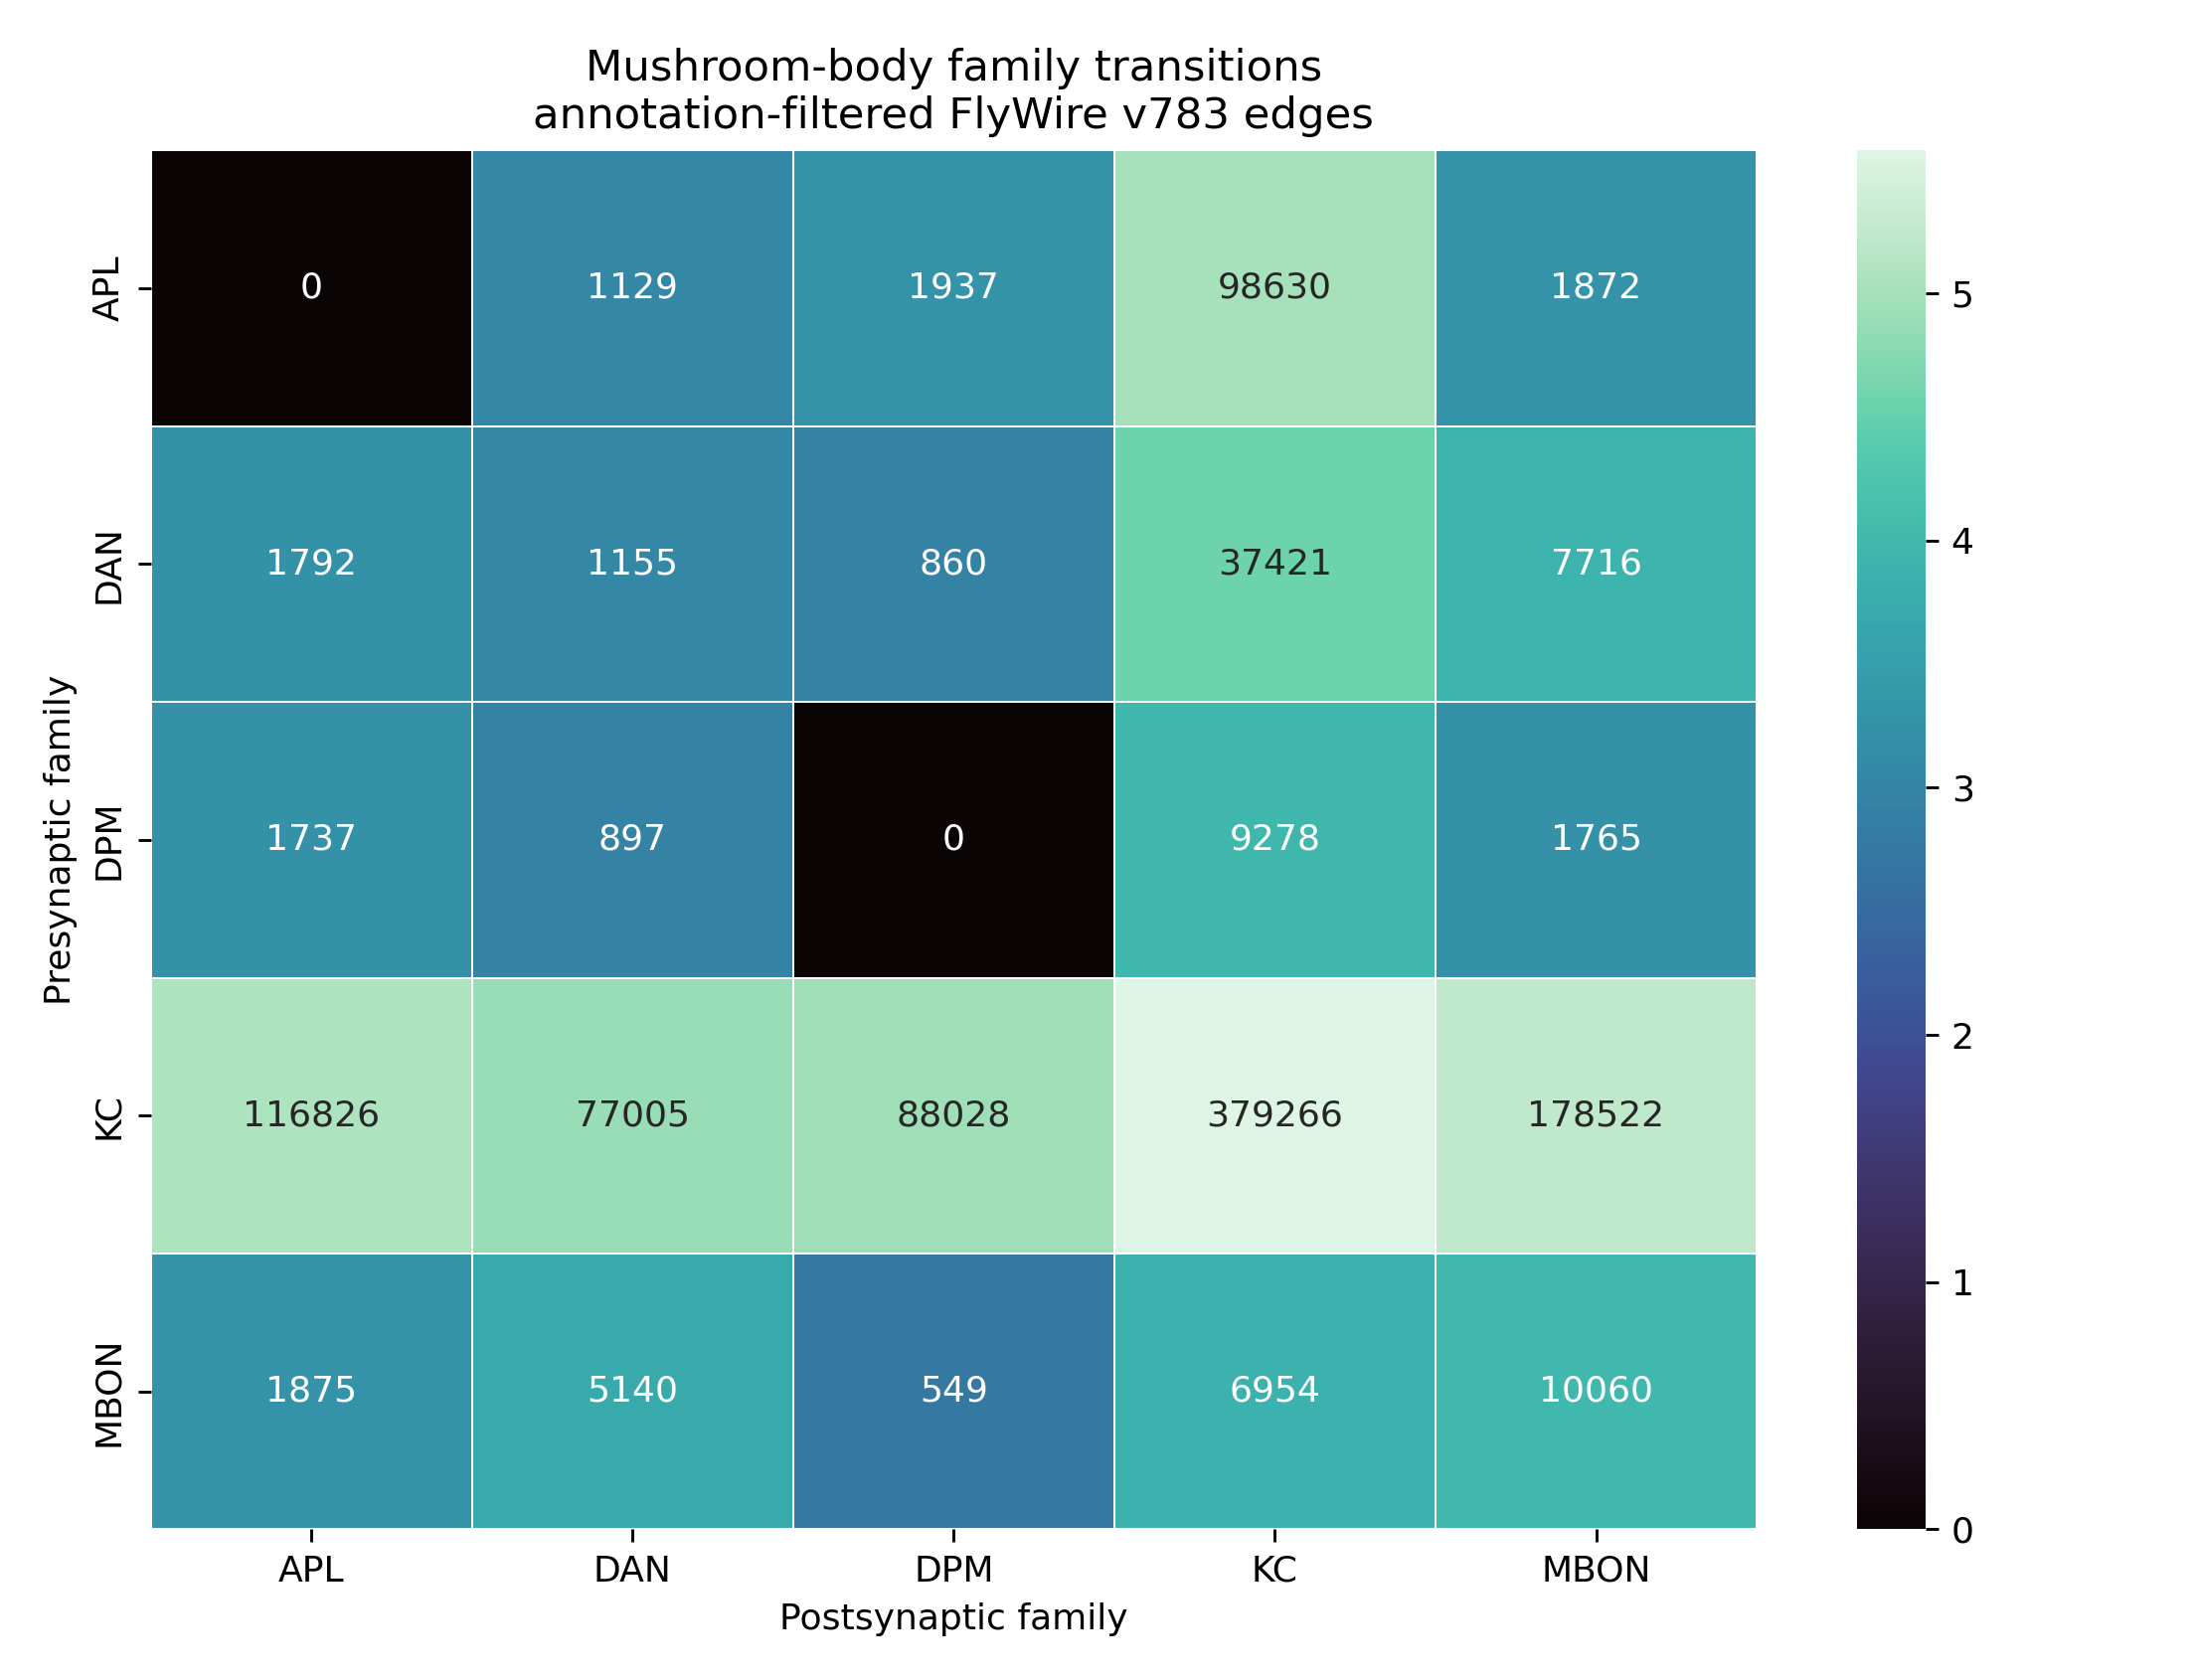
\includegraphics[width=0.48\linewidth]{figures/Fig12_mb_family_transition_heatmap.png}
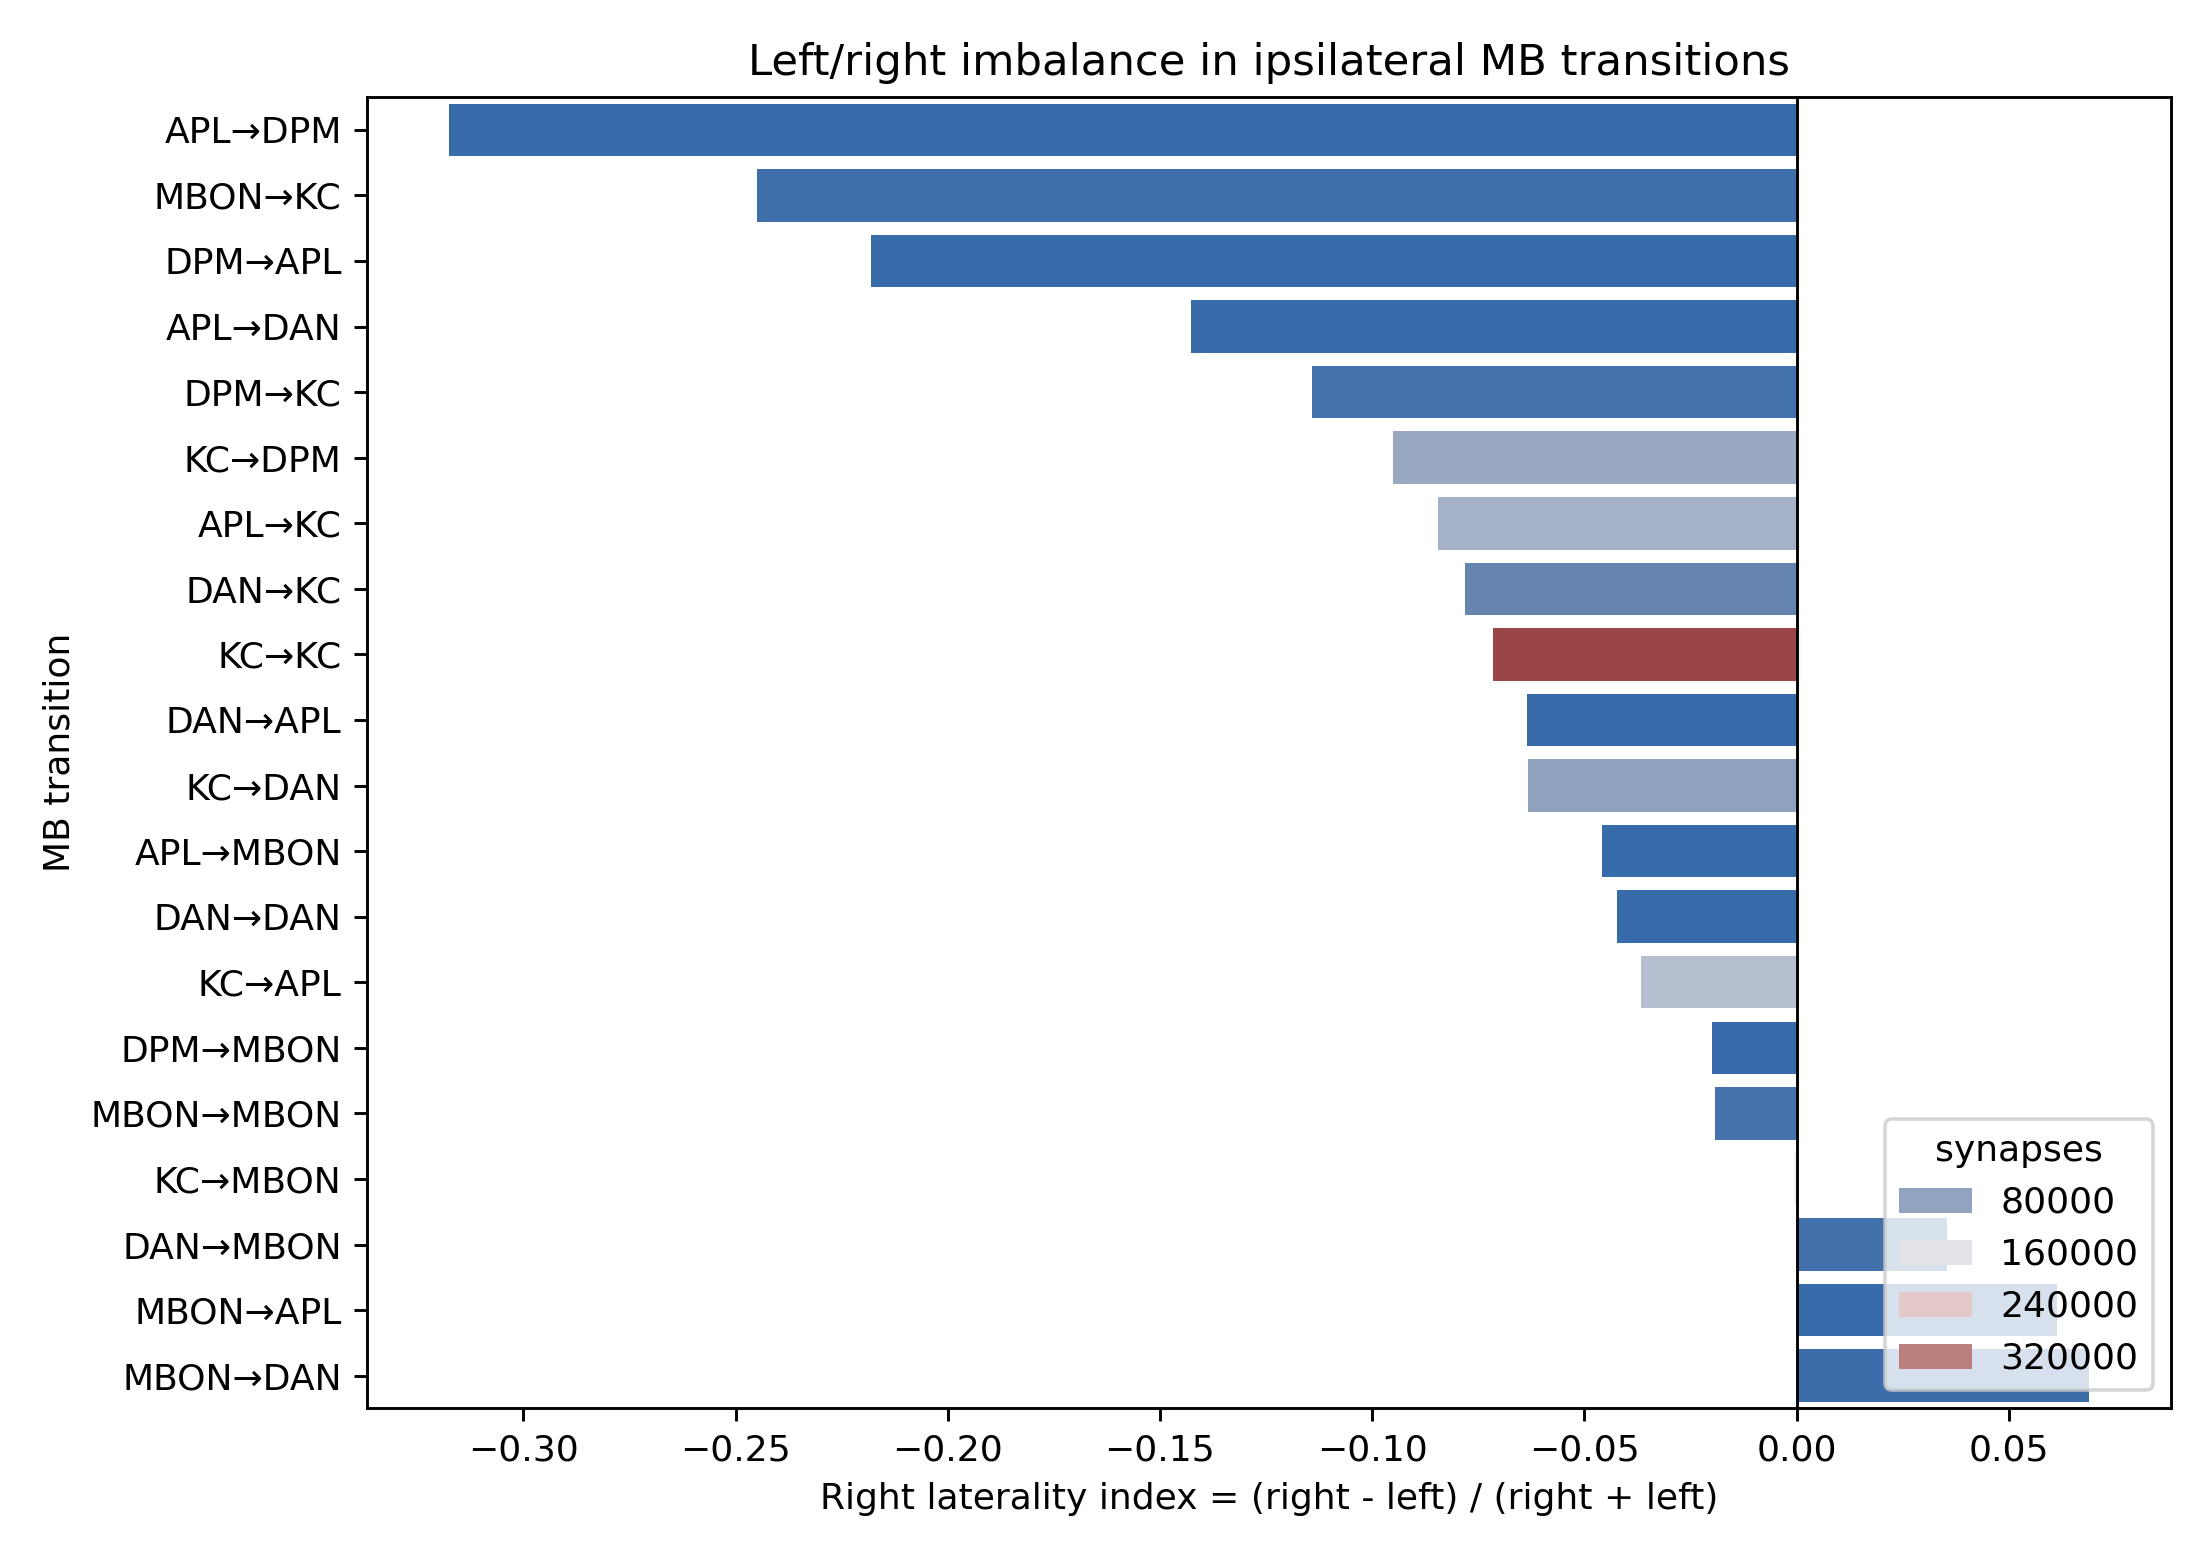
\includegraphics[width=0.48\linewidth]{figures/Fig13_mb_transition_laterality.png}
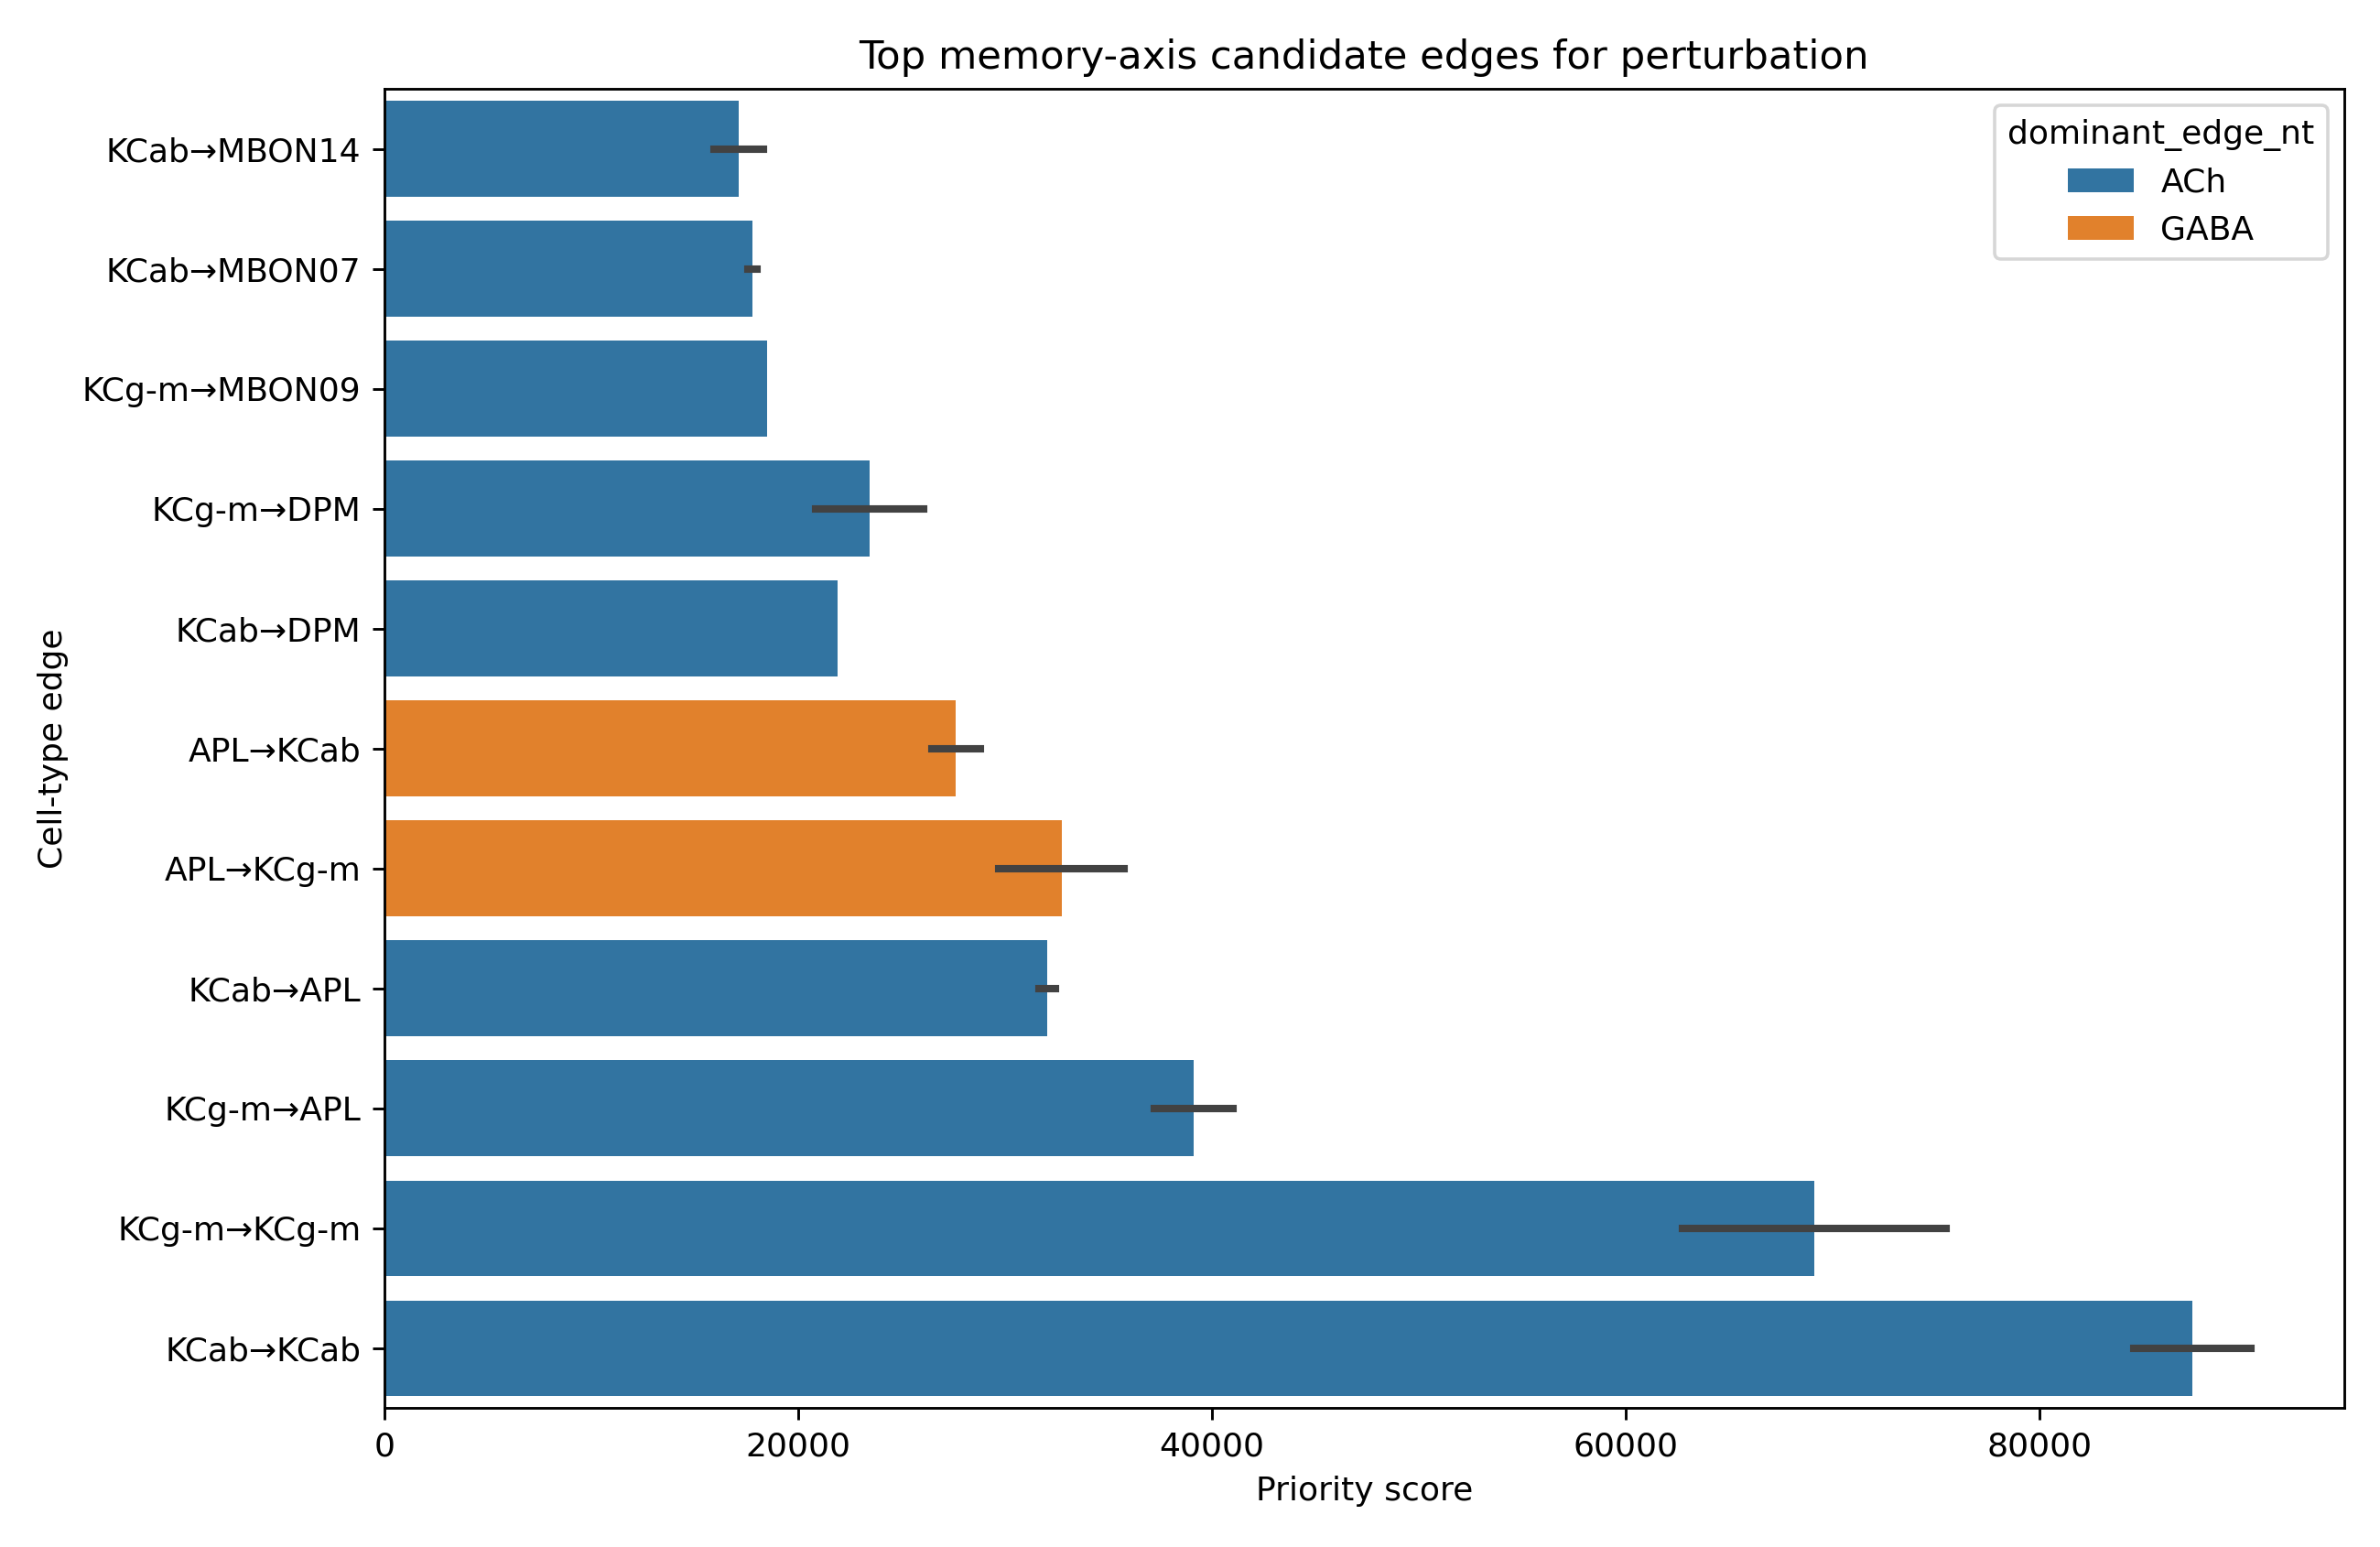
\includegraphics[width=0.48\linewidth]{figures/Fig14_memory_axis_candidate_targets.png}
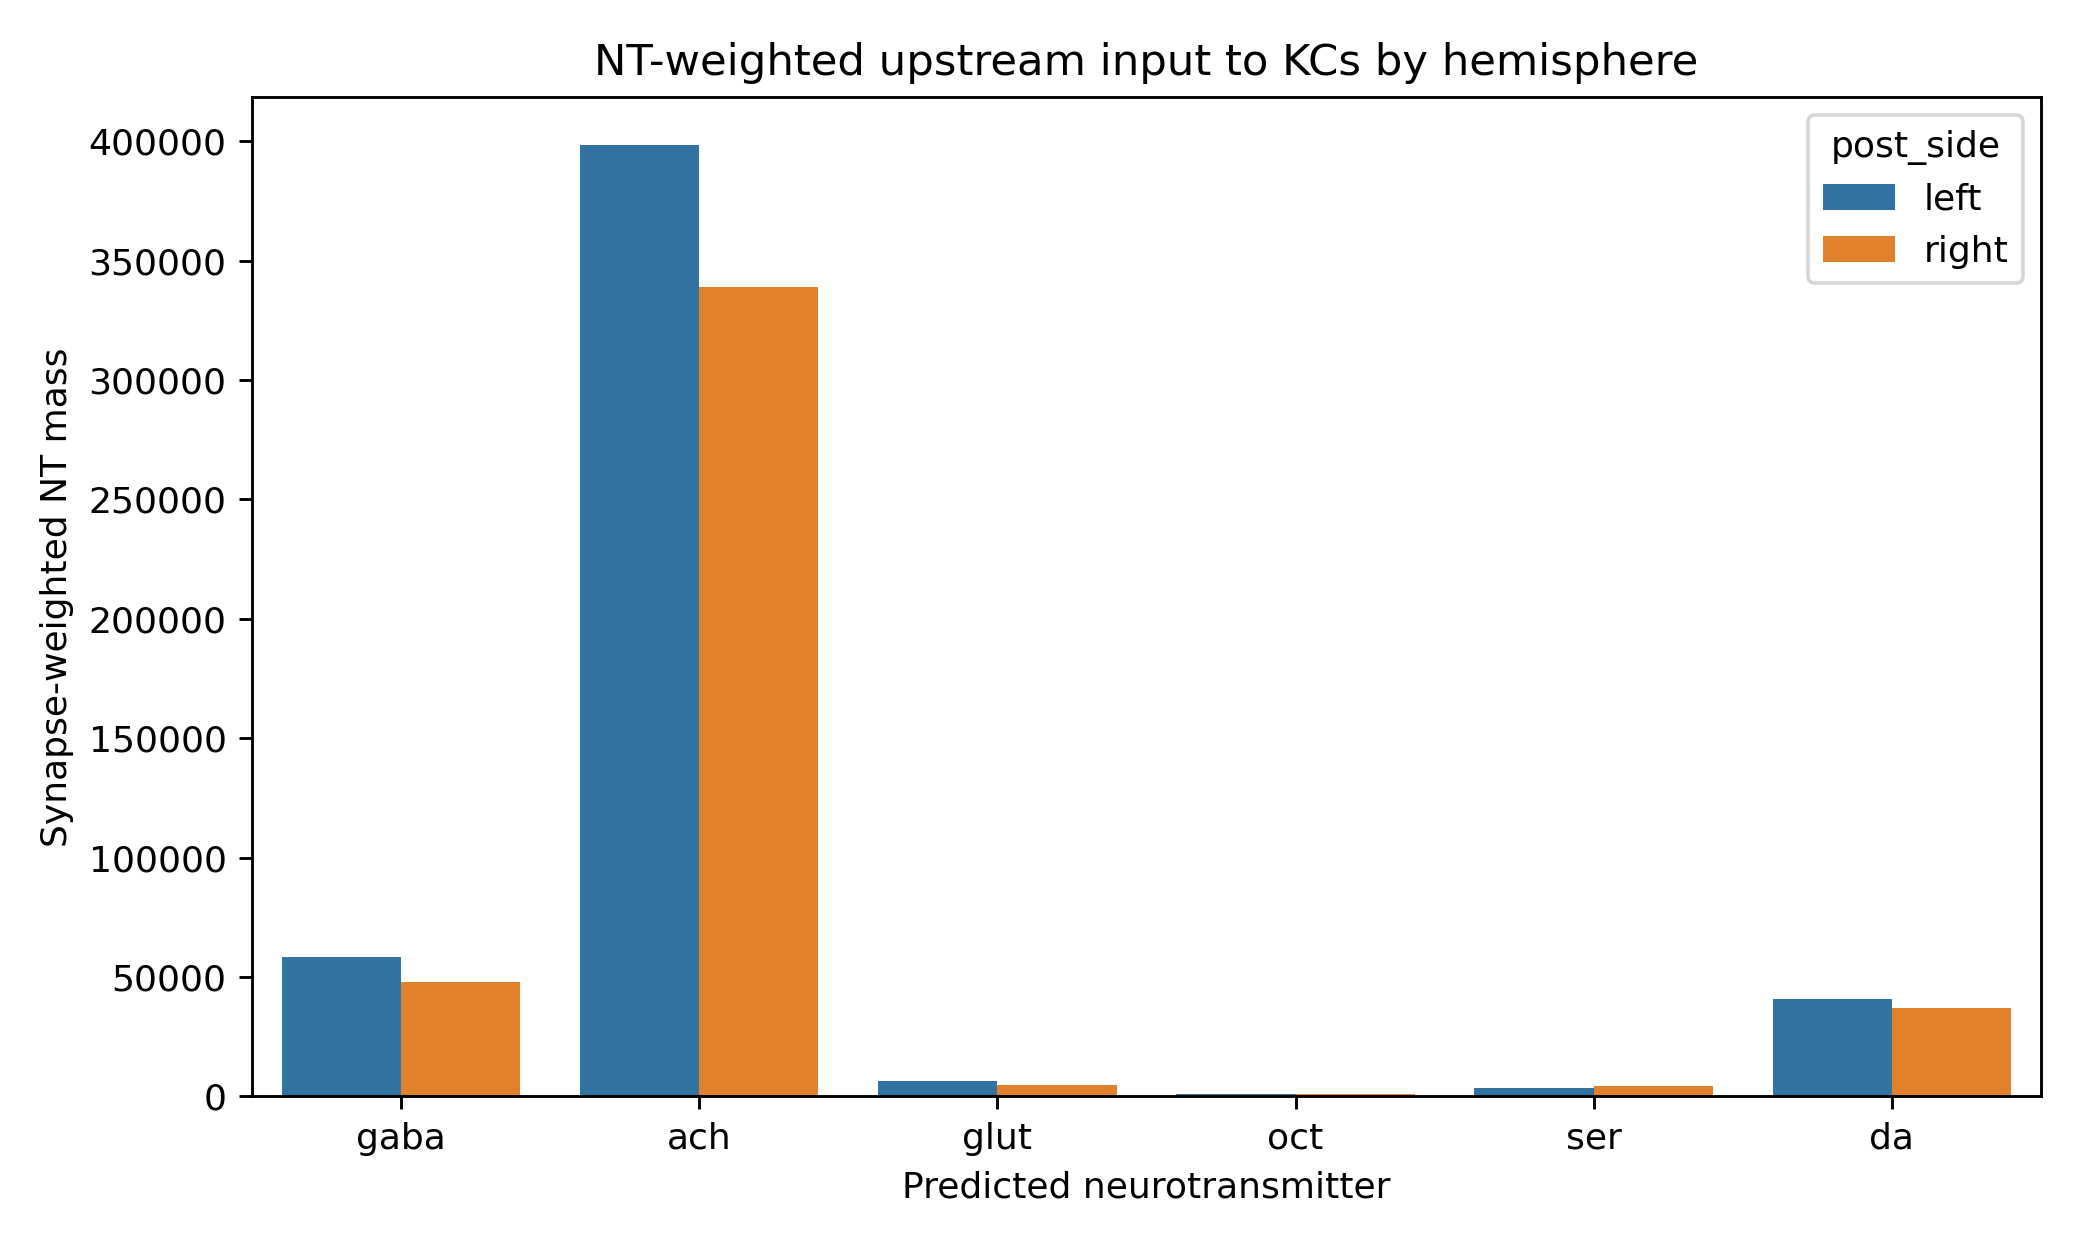
\includegraphics[width=0.48\linewidth]{figures/Fig15_kc_upstream_nt_by_side.png}
\caption{\textbf{Connectome-constrained circuit mining and food-odour memory simulation.}
\textbf{a},~Mushroom-body family transition heatmap from FlyWire v783 aggregated connections.
\textbf{b},~Ipsilateral transition laterality; negative values indicate left enrichment and positive values indicate right enrichment.
\textbf{c},~Top memory-axis candidate transitions used to define perturbation conditions.
\textbf{d},~Synapse-weighted neurotransmitter mass in KC upstream input by hemisphere. Supplementary videos in \texttt{paper/video/food\_memory\_cs\_plus\_left.mp4} and \texttt{paper/video/food\_memory\_cs\_plus\_right.mp4} show mirrored food-odour search simulations.}
\label{fig:mb_circuit_sim}
\end{figure}

\FloatBarrier

% ════════════════════════════════════════════════════════════════════════
%  DISCUSSION
% ════════════════════════════════════════════════════════════════════════
\section*{Discussion}

\subsection*{Multi-scale representation learning for connectomics}

Our first contribution is a multi-scale analytical framework that progresses from single-neuron skeleton analysis to whole-brain connectivity profiling. The hierarchical graph neural network architecture (HGNNA) with skeleton decomposition reduces memory cost by over 100$\times$, enabling contrastive learning on finely sampled skeletons with 3,500 nodes---covering 96.37\% of neurons in FlyWire. Finely sampled skeletons improve classification accuracy by up to 31\% over coarse skeletons, with the largest gains in the visual system (Tm: 70\% $\to$ 100\%), demonstrating that the detailed morphological information captured by high-resolution skeletons is essential for distinguishing neuronal types.

The resulting topology embeddings---which are invariant to coordinate symmetries that confound morphological representations---provide a robust foundation for downstream connectivity analysis. The observation that topology outperforms morphology in unsupervised clustering (Silhouette score improvement from $-0.048$ to $0.090$ for KCs) while maintaining comparable supervised classification accuracy demonstrates that coordinate-free representations capture the essential structural information while discarding confounding spatial variation. The sensitivity analysis reveals three specific confounds in morphological representations: (i)~developmental lineage differences in dendritic segments, which create sub-clusters within KC types; (ii)~hemispheric mirror symmetry, which separates left and right neurons of the same type; and (iii)~positional gradients in the optic lobe, where soma y-coordinate correlates significantly with the latent representation. By removing coordinates, the topological representation eliminates all three confounds simultaneously, and its robustness to reduced labelling (stable accuracy at 10\% labels vs.\ 13\% degradation for morphology) makes it particularly suitable for the common scenario where expert annotations are scarce.

The multi-scale nature of the framework is important: the skeleton-level HGNNA captures neuron-intrinsic structural identity (``what does this neuron look like?''), while the connectivity-graph GNN captures circuit-level relational identity (``what role does this neuron play in the network?''). The two representations are largely orthogonal ($r < 0.3$), and their combination improves classification by +6.6\% to +14.1\% over topology alone, confirming that morphology and connectivity provide complementary information about neuronal identity.

\subsection*{An empirical feature-scale pattern for connectome analysis}

Our second contribution is an empirically grounded feature-scale matching pattern: the optimal scale for NT-based connectivity features matches circuit architecture. Modulatory circuits favour local features; hierarchical circuits favour global features. The sign of $\Delta$ (local $-$ global accuracy) serves as a diagnostic: $\Delta > 0$ indicates a population organized by compartment-specific modulatory input (KC: $+9.6\%$; Central: $+7.0\%$), while $\Delta < 0$ indicates a population organized by position in processing hierarchies (Tm: $-20.1\%$). This pattern was observed across three datasets (FlyWire, Hemibrain, MICrONS), providing practical guidance for the growing number of labs working with dense connectome data\cite{dorkenwald2024flywire,scheffer2020hemibrain,microns2021cortical}. The Hemibrain replication ($\Delta = +14.1\%$ for KC) is particularly compelling because it uses an independently reconstructed brain with different segmentation algorithms and annotation pipelines. The MICrONS result ($\Delta = +0.4\%$) is consistent with mammalian cortex following a canonical microcircuit architecture with more uniform E/I ratios, where the local--global distinction is less relevant.

The connectivity-graph GNN provides an independent, end-to-end validation: NT features alone achieve only 40.7\% without graph structure, but 77.4\% \textit{with} graph message passing---a +36.7 percentage point synergy demonstrating that NT connectivity is fundamentally relational. This result has a deeper biological implication: a neuron's NT identity alone provides limited classification information (40.7\%, barely above the 11.1\% random baseline for 9 classes), but when combined with the NT identities of its synaptic partners---i.e., the local circuit's NT composition---classification nearly doubles. This means that \textit{NT connectivity}---``who uses what NT to connect to whom''---encodes far more cell-type information than individual NT identity alone, consistent with the known organization of the mushroom body where different KC types receive input from distinct projection neuron populations with different NT profiles\cite{li2020kc_types,aso2014mushroom}.

Importantly, for KCs, the 86D fusion vector (80.2\%) performs \textit{below} NT Neighbor alone (88.9\%), because the fusion includes topology and NT Circuit features that are less informative for this population. This reinforces the same pattern: for modulatory circuits, adding global context can actively dilute the local signal. This counter-intuitive result---that more features can reduce accuracy---underscores the importance of matching feature scale to circuit architecture rather than naively concatenating all available features.

\subsection*{Pervasive lateralization and its functional implications}

Our third---and most biologically significant---contribution is the discovery of pervasive NT lateralization in the mushroom body and beyond. Five observations constrain the interpretation.

\textit{First}, serotonin right-enrichment is universal across all 9 KC types (binomial $p = 0.004$) and extends to 7/7 testable central-brain neuron types. This universality---spanning all three lobe systems ($\alpha'\beta'$, $\alpha\beta$, $\gamma$) and extending beyond the mushroom body---suggests a brain-wide hemispheric gradient in serotonergic innervation, not merely a MB-specific effect. The gradient is strongest in the $\alpha'\beta'$ lobe (Cohen's $d$ up to $+1.45$, Cliff's $\delta = 0.77$) and weakest in $\gamma$ ($d = 0.56$), consistent with a graded rather than binary lateralization. The resolution of KC$\alpha'\beta'$-m as a separate type strengthens this conclusion: all three $\alpha'\beta'$ types (ap1, ap2, m; combined $n = 916$) show concordant, extreme serotonin right-enrichment ($d = +1.34$ to $+1.45$). By contrast, visual neurons show the opposite pattern (Ser L$>$R), consistent with the distinct circuit architecture of the optic lobe and further supporting the specificity of the central-brain gradient.

\textit{Second}, the lateralization follows a functional gradient aligned with memory processing: the $\alpha'\beta'$ lobe (memory consolidation; Cohen's $d$ up to $+1.45$) is most lateralized, the $\gamma$ lobe (short-term memory; $d = 0.56$) is least, and the $\alpha\beta$ lobe (long-term memory; $d = 0.30$) is intermediate. The compartment-level analysis (Table~\ref{tab:lobe}) confirms this gradient with increased statistical power. The co-occurrence of serotonin right-enrichment and glutamate left-bias in the same types suggests coordinated hemispheric specialization of excitatory and modulatory inputs. The asymmetry is also multi-dimensional: while serotonin shows the most consistent directionality, glutamate left-bias (7/9 types, 7 individually significant, $d$ up to $-1.47$) and GABA asymmetry (6/9 significant) indicate that lateralization extends beyond a single transmitter system.

\textit{Third}, the lateralization is input-specific. Analysis of 563,235 KC output synapses reveals that all KC outputs are 100\% cholinergic (ACh = 1.0) with zero variance across all neurons and types. This confirms that the asymmetry arises from differential upstream modulation rather than intrinsic KC properties. KCs are a homogeneous cholinergic population whose functional diversity arises entirely from the NT composition of their inputs---a finding that reinforces the feature-scale matching pattern established above, where local NT input features (NT Neighbor) proved most informative for KC classification.

\textit{Fourth}, the results are robust across multiple independent validation approaches spanning frequentist, Bayesian, and model-based paradigms. GPU-accelerated permutation tests (10,000 shuffles) confirmed 30/54 significant effects. Bootstrap BCa confidence intervals excluded zero for 41/54 tests, including all 9/9 serotonin tests. Bayesian $t$-tests yielded extreme evidence (BF$_{10} > 100$) for 25/54 tests, with serotonin extreme in 7/9 types. SIMEX measurement-error extrapolation preserved serotonin direction in 9/9 types even at zero measurement error. Gold's iterative deconvolution of the classifier confusion matrix confirmed 30/54 significant effects with 100\% direction preservation for large effects. Hotelling's $T^2$ multivariate tests on the full 6D NT profile confirmed significant hemispheric differences in all 9/9 types (all $p < 10^{-13}$). The convergence of these seven orthogonal methods---each addressing a different potential artifact (label bias, sampling variability, prior sensitivity, measurement error, classifier confusion, multivariate structure)---provides strong evidence against statistical artifacts (Extended Data Fig.~\ref{fig:ext_convergence}).

\textit{Fifth}, the upstream decomposition reveals that the serotonin asymmetry in both KC$\alpha'\beta'$-ap1 and the newly resolved KC$\alpha'\beta'$-m is driven by a 9.5-fold enrichment of dopaminergic neuron (DAN) input to right-hemisphere KCs (Fisher's exact $p = 2.2 \times 10^{-5}$ for ap1; $p = 3.5 \times 10^{-7}$ for KC$\alpha'\beta'$-m). The DAN imbalance extends broadly: KC$\gamma$-d (7.8$\times$), KC$\gamma$-m (4.8$\times$), and KC$\alpha\beta$-s (3.9$\times$) all show significant DAN enrichment. Since DANs convey valence signals to specific MB compartments\cite{aso2014mushroom,modi2020dopamine_kc}, this hemispheric DAN imbalance suggests that reward and punishment signals may be processed asymmetrically.

The functional implications are striking. Serotonergic modulation of the MB---primarily via the DPM neuron\cite{keene2006dpm}---is specifically required for anesthesia-resistant memory and acts through $\alpha'\beta'$ KCs\cite{waddell2013serotonin}. Our discovery of lateralized serotonergic input to this exact KC population provides a structural substrate that could underlie the lateralized long-term memory formation first reported by Pascual et al.\cite{pascual2004lateralized}. The graded correspondence between lateralization strength and memory function---$\alpha'\beta'$ (consolidation) $>$ $\alpha\beta$ (long-term) $>$ $\gamma$ (short-term)---suggests that the degree of hemispheric specialization scales with the computational demands of the memory process.

The new connectome-constrained circuit mining strengthens this interpretation. The most abundant ipsilateral transitions do not show a uniform hemispheric bias; instead, recurrent and feedback-like modules (KC--KC, KC--APL, APL--KC, KC--DPM and DPM--KC) are left-biased, whereas DAN--MBON and MBON--DAN transitions are weakly right-biased and KC--MBON output is nearly balanced. This pattern is consistent with a two-axis model in which one hemisphere preferentially stabilizes or gates memory traces through recurrent feedback, while the other contributes more strongly to modulatory output and decision-state switching. The food-odour simulations translate this structural model into behavioural predictions: manipulations of the left KC--APL--DPM feedback module should change continuous food-approach margins, especially when the learned sugar cue is weak and a competing odour is strong. These simulations are not a substitute for closed-loop neural recordings, but they provide a concrete bridge from static connectome asymmetry to testable behaviour.

We further implemented a CyberFly-style multimodal benchmark to clarify the level at which embodied phenomena are reproduced. Rather than assuming that the connectome alone generates complete behaviour, the benchmark separates sensory seeding, connectome propagation, descending-neuron readout and body-level control. Olfactory ORN seeds, LC/LPLC visual projection seeds, gustatory seeds and mechanosensory seeds were propagated through the FlyWire v783 network and scored against descending, memory-axis, visual, gustatory and mechanosensory readout sets. This reproduced the expected qualitative separation of sensory channels: visual and mechanosensory seeds produced stronger descending readout than olfactory food-memory seeds, whereas olfactory seeds produced a larger memory-axis component. Embodied videos were then generated for food-odour approach, visual object tracking and front-leg grooming proxies. The visual and grooming videos should be interpreted as readout-constrained behavioural proxies, not as evidence that a full motor programme emerges from the connectome without additional controller assumptions.

We next resolved the descending readout into named DN families, because these neurons are the anatomical interface through which brain computations can influence walking, steering, escape, grooming and feeding-like motor programmes. The sensory modalities recruited distinct DN-family profiles. Olfactory food-memory seeds recruited only 58 descending neurons and produced weak descending mass (0.0115), consistent with a primarily central memory-axis computation before motor output. In contrast, visual-object seeds recruited 704 descending neurons (descending mass 0.204), dominated by DNg, DNge and DNp families; gustatory seeds recruited 638 descending neurons (descending mass 0.255), with DNge contributing 51.4\% of descending mass; and mechanosensory seeds recruited 769 descending neurons (descending mass 0.463), with DNg contributing 51.0\%. The DN laterality indices were modest but non-zero, ranging from +0.049 for olfactory food-memory input to -0.103 for gustatory input. These results provide a mechanistic intermediate between static connectome structure and behaviour: modality-specific inputs do not merely activate generic central-brain targets, but preferentially access distinct descending interfaces. They remain predictions of connectome-constrained propagation and therefore require targeted DN perturbation or recording for causal validation.

\begin{figure}[t]
\centering
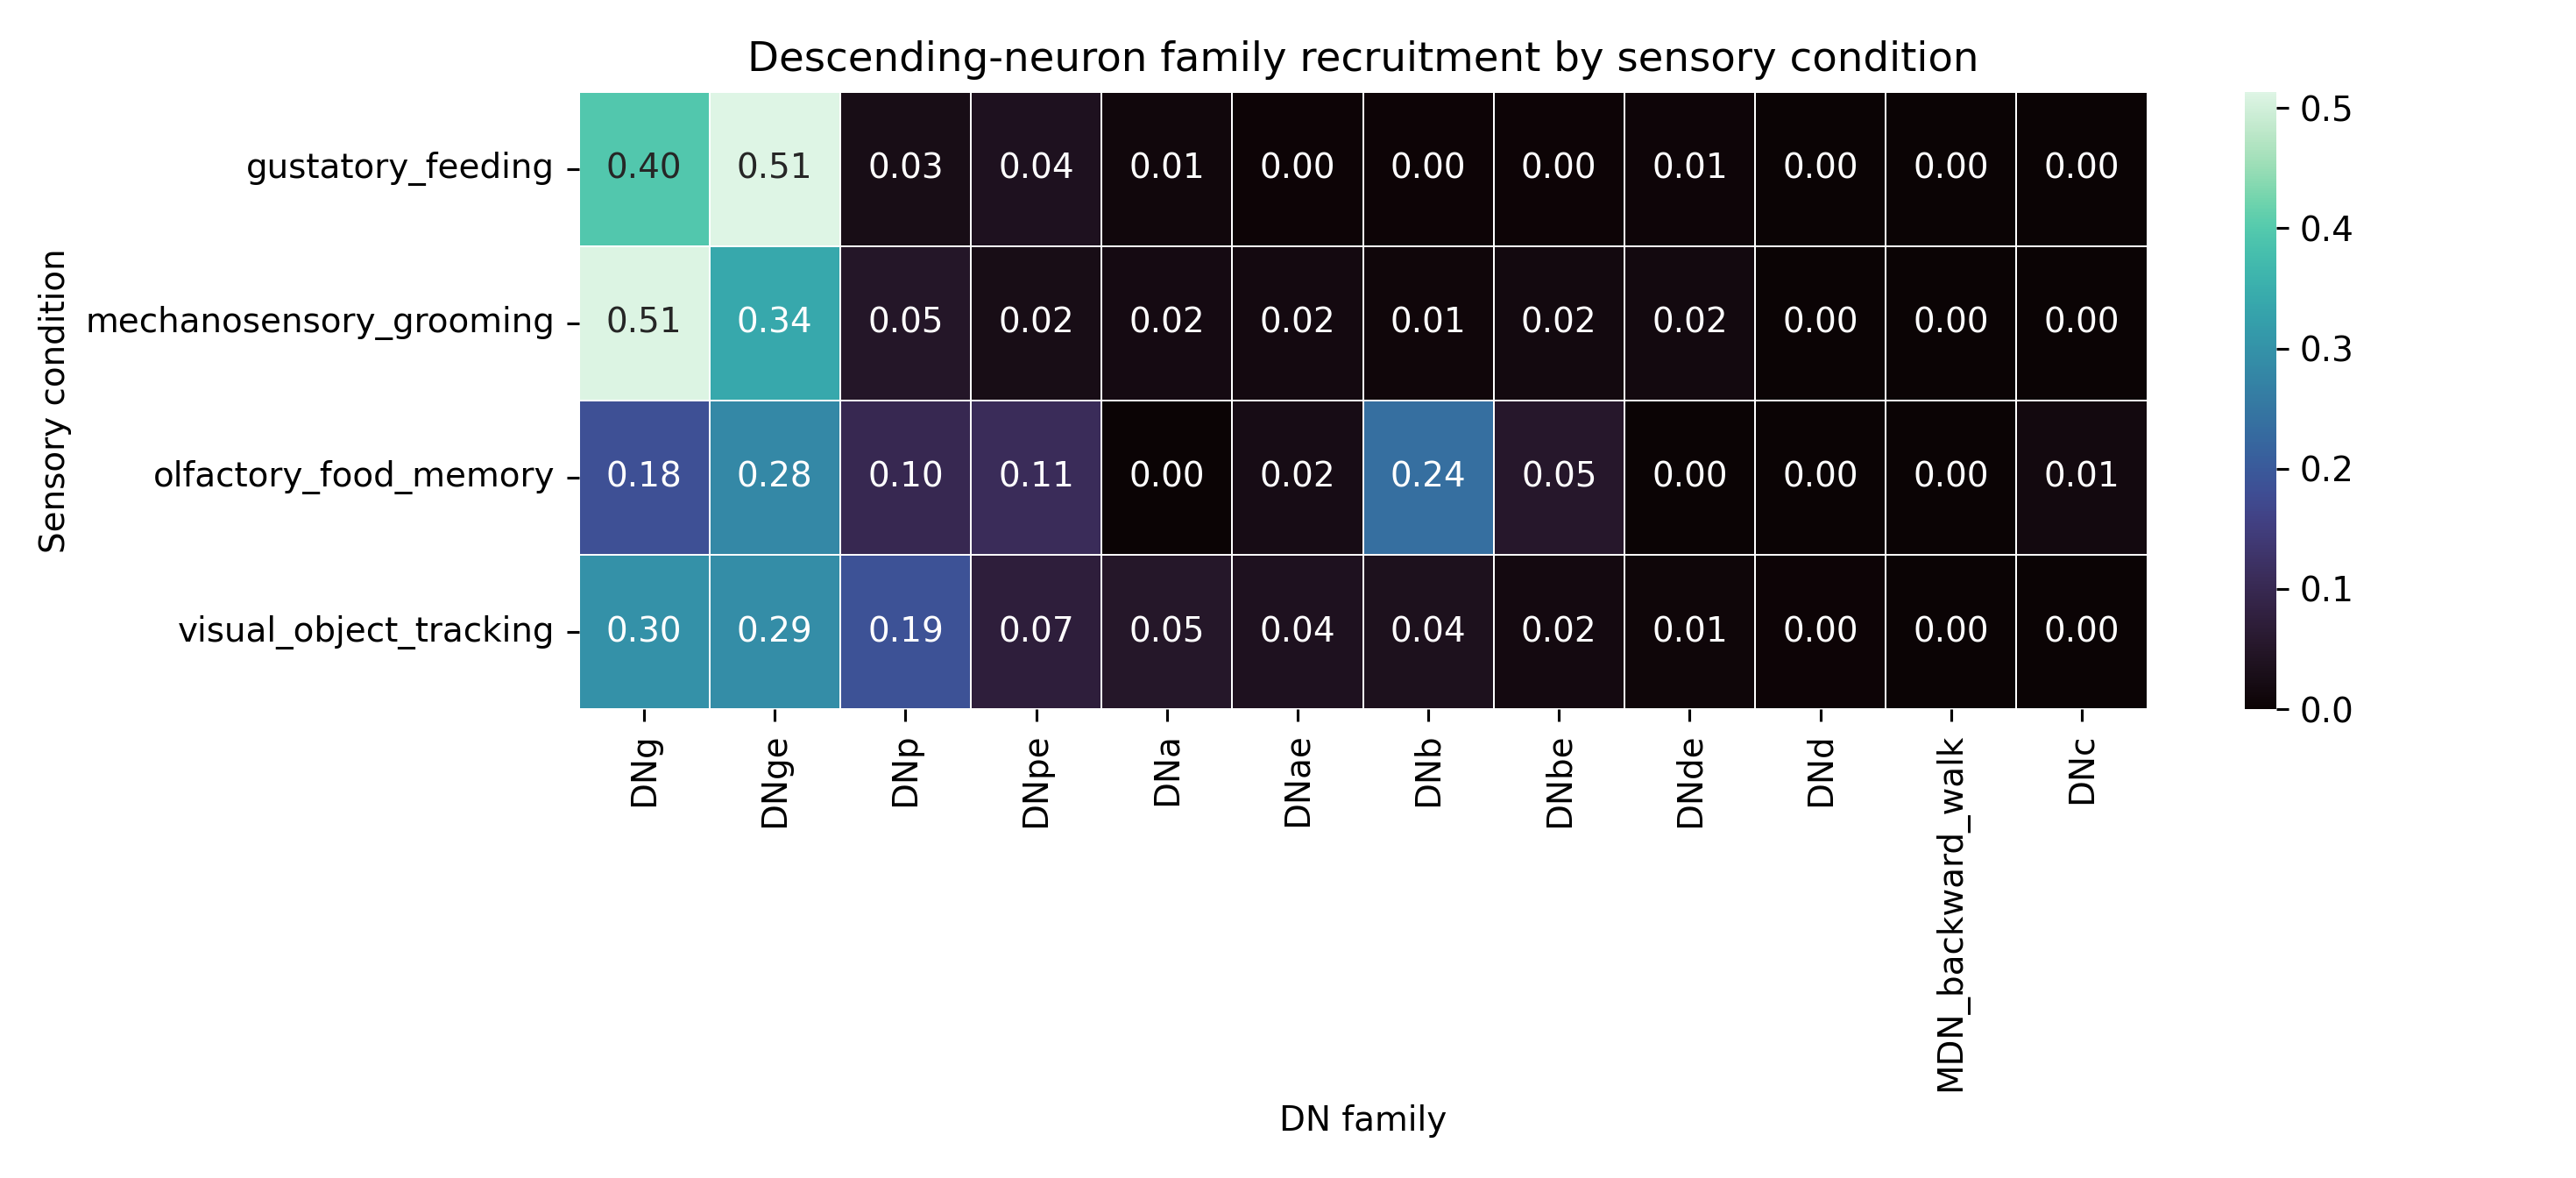
\includegraphics[width=0.58\linewidth]{figures/Fig16_dn_family_readout_heatmap.png}
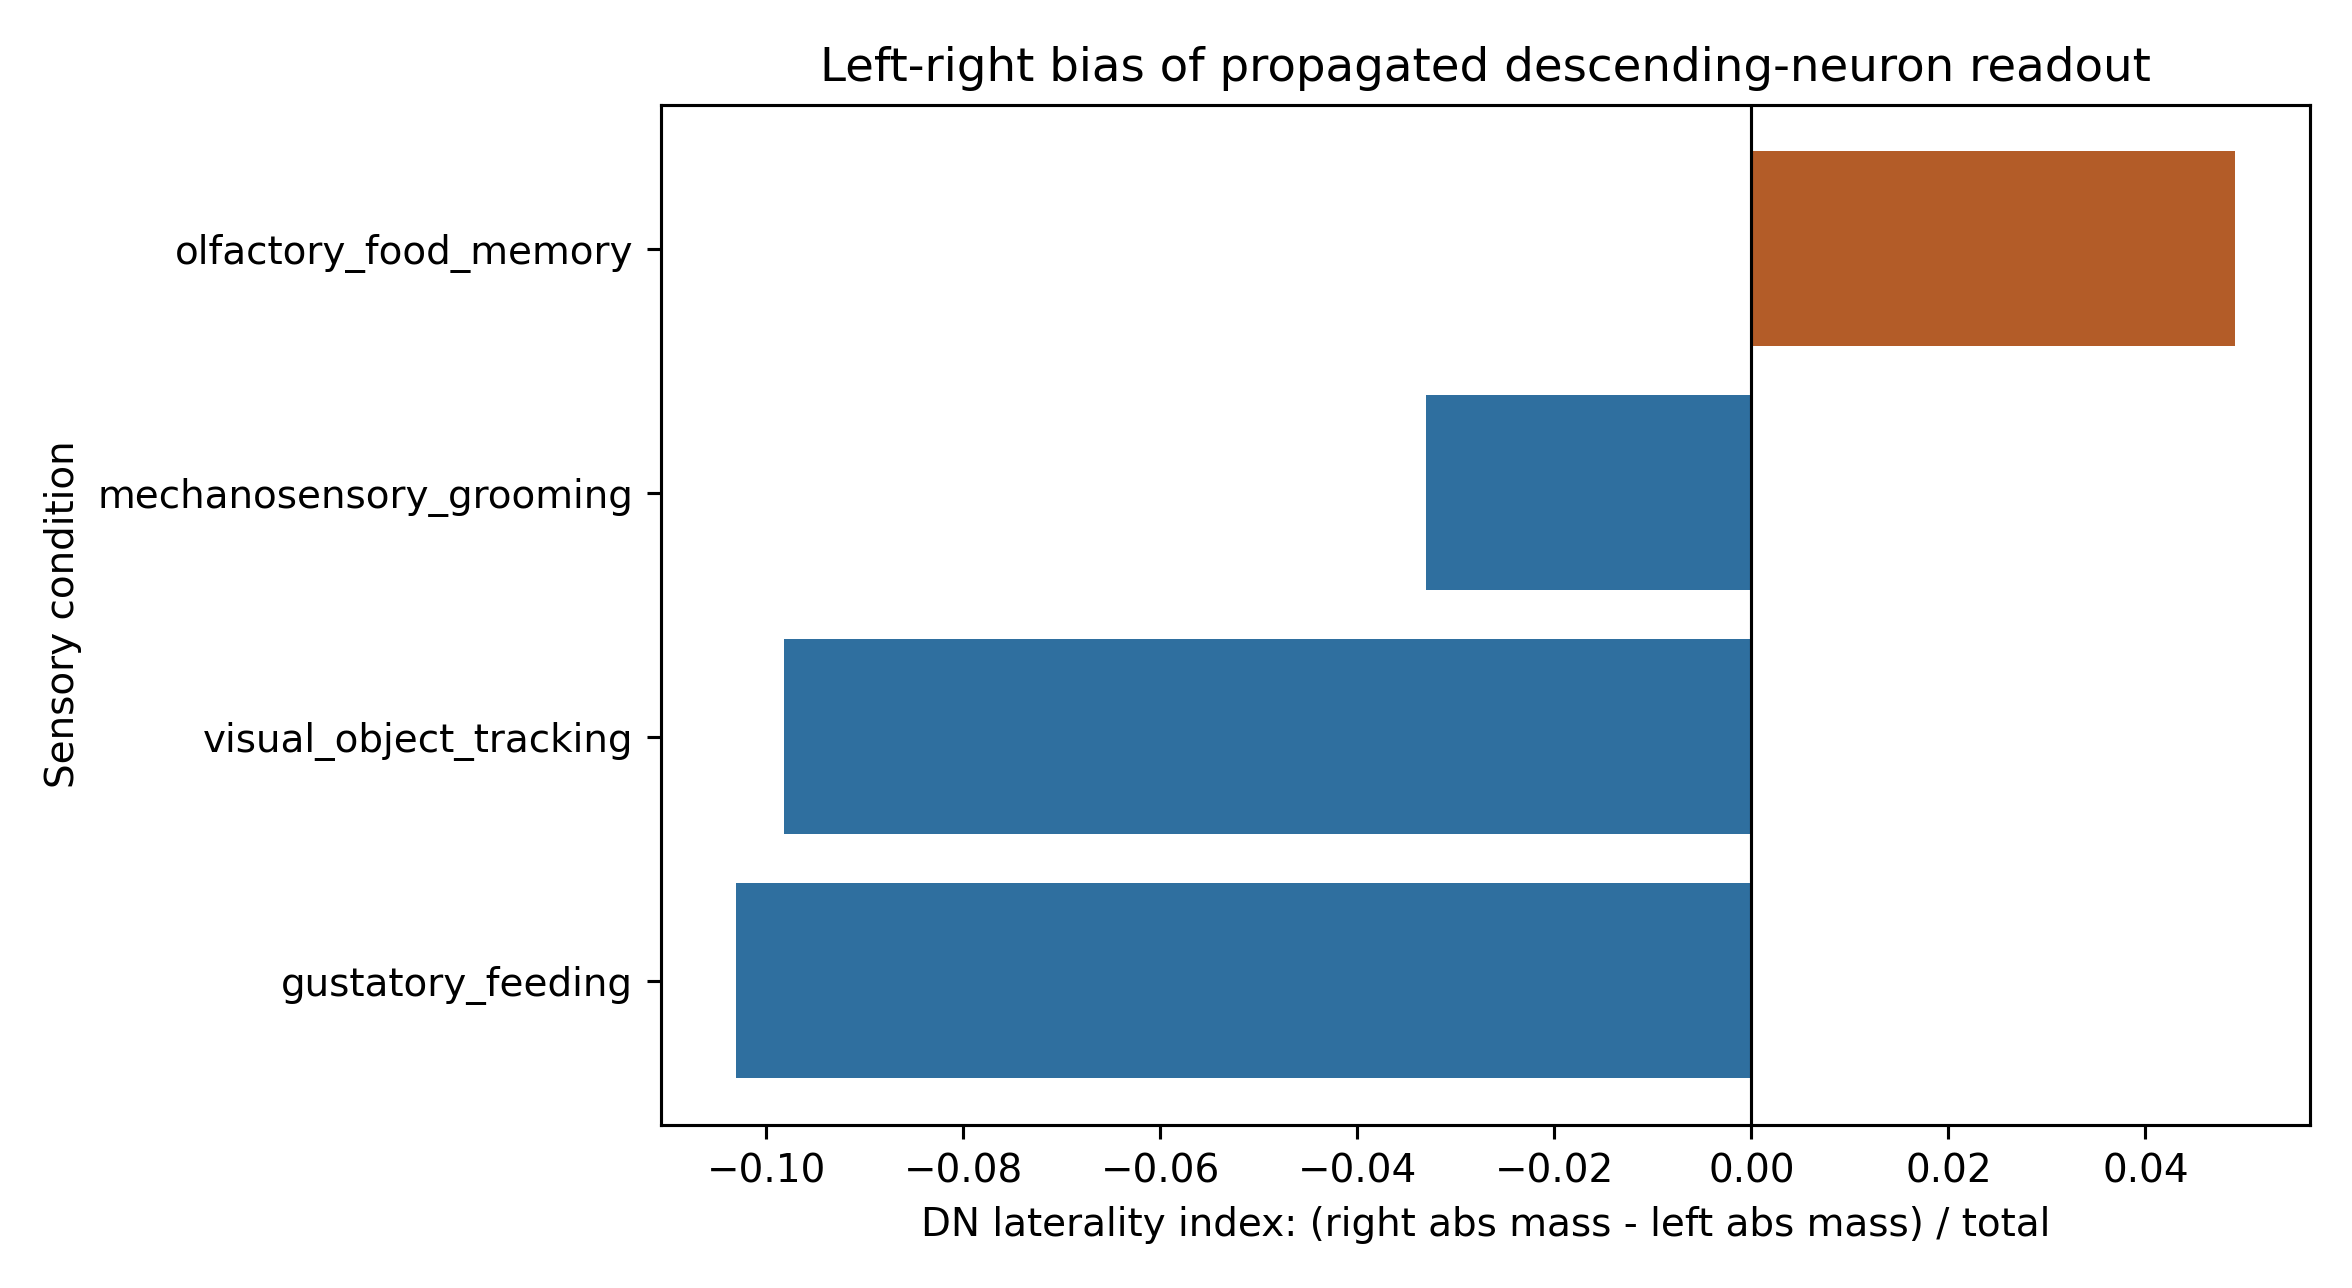
\includegraphics[width=0.39\linewidth]{figures/Fig17_dn_laterality_index.png}
\caption{\textbf{Modality-specific recruitment of descending-neuron interfaces.} Left, family-level absolute response fractions for descending neurons recruited by olfactory food-memory, visual-object, gustatory and mechanosensory seed sets. Right, hemispheric laterality index of descending response mass, computed as \((M_R-M_L)/(M_R+M_L)\). The figure summarizes connectome-constrained propagation predictions; it should be interpreted as a target-prioritization readout rather than a causal behavioural proof.}
\label{fig:dn_readout}
\end{figure}

\subsection*{Relationship to prior work on brain lateralization}

Our findings sit at the intersection of two converging lines of evidence. In \textit{Drosophila}, Pedigo et al.\cite{pedigo2023bilateral_elife} showed quantitatively that KCs are the primary source of bilateral connectivity differences in the larval brain---removing KCs from the analysis eliminated detectable left--right differences. Winding et al.\cite{winding2023larva} confirmed this in the full larval connectome. Our results extend these observations to the adult brain and, critically, add NT specificity: we identify \textit{which} transmitter systems (serotonin, glutamate) and \textit{which} lobe systems ($\alpha'\beta'$, not $\gamma$) contribute. The finding that central-brain neurons share the serotonin lateralization pattern further extends the scope beyond the MB, suggesting that the lateralization program operates at a broader developmental scale.

In vertebrates, brain lateralization is now understood as a multi-scale phenomenon. Karolis et al.\cite{karolis2019lateralisation} mapped functional lateralization across the human cortex and showed that lateralized regions exhibit reduced contralateral connectivity---suggesting an evolutionary trade-off between hemispheric specialization and inter-hemispheric communication. Wan et al.\cite{wan2024microstructural} demonstrated that cortical microstructural asymmetry follows an anterior--posterior gradient and correlates with functional lateralization. Our discovery of NT-level lateralization in the MB adds a molecular dimension to this picture: lateralization is not merely a property of wiring topology but extends to the neurotransmitter identity of synaptic inputs.

The cross-species comparison is instructive. MICrONS mouse V1 shows no local--global dissociation ($\Delta = 0.4\%$), consistent with mammalian cortex following a canonical microcircuit architecture with uniform E/I ratios\cite{microns2021cortical}. This may reflect a fundamental difference: the insect MB uses discrete modulatory compartments to encode memory valence\cite{aso2014mushroom}, creating natural ``fault lines'' along which lateralization can emerge, whereas mammalian cortex uses a more uniform columnar architecture. The Hemibrain dataset, while providing strong structural validation of KC type organization (Spearman $r = 0.83$ with FlyWire), is a single right hemisphere without per-synapse NT predictions, precluding direct cross-validation of NT lateralization. Future connectome reconstructions of multiple individual brains will be essential for distinguishing stereotyped from stochastic asymmetry.

Linneweber et al.\cite{linneweber2020asymmetry} demonstrated stochastic inter-individual variation in visual circuit asymmetry in \textit{Drosophila}; our analysis, being restricted to a single brain, cannot distinguish stereotyped from stochastic asymmetry. However, the universality of serotonin right-enrichment across all 9 KC types---spanning three independently specified lobe systems---and its extension to 7/7 central-brain types argues strongly against a purely stochastic origin and favours a developmentally programmed mechanism.

\subsection*{Caveats}

Seven limitations apply. (i)~We analyse a single brain (FlyWire v783); inter-individual variability---known to exist in \textit{Drosophila} visual circuits\cite{linneweber2020asymmetry}---cannot be assessed. However, the universality of serotonin right-enrichment across all 9 KC types and 7/7 central-brain types argues against a purely stochastic origin. (ii)~The per-synapse NT classifier has non-uniform accuracy ($\sim$80\% for serotonin vs $>$90\% for ACh/GABA)\cite{eckstein2020neurotransmitter}. The serotonin effects are confirmed by non-parametric Cliff's delta, permutation tests, split-half reliability, and a Monte Carlo robustness analysis (500 rounds with confusion-matrix correction and Dirichlet noise) that maintained the 9/9 R$>$L consensus in 100\% of rounds even at 30\% per-synapse accuracy. Glutamate left-bias, relying on a higher-accuracy prediction, may be the most robust signal. (iii)~The Hemibrain dataset is a single right hemisphere without per-synapse NT predictions, precluding direct cross-validation of NT lateralization. Structural type organization is consistent between datasets (Spearman $r = 0.83$). (iv)~The binomial test for serotonin consistency assumes independence across types; the $p$-value should be interpreted as an upper bound. (v)~Skeleton representation figures (Fig.~1--3) are based on a separate training pipeline; the topology embeddings used as GNN node features are from this pipeline. (vi)~The DAN--serotonin co-occurrence in upstream analysis could reflect classifier limitations, genuine co-transmission, or annotation granularity. (vii)~The food-odour simulation is a reduced embodied assay: the sugar source is represented as an odour-conditioned target rather than a consumable object, and the FlyGym controller implements a low-dimensional sensorimotor policy rather than a full spiking closed-loop brain model. It is therefore appropriate for generating perturbation hypotheses and videos, but not for claiming behavioural causality without real experiments.

\subsection*{Outlook}

The multi-scale framework and feature-scale matching pattern generate testable predictions for upcoming connectomes. For the male \textit{Drosophila} connectome, we predict that the local--global dissociation ($\Delta > 0$ for KC, $\Delta < 0$ for Tm) will be preserved, as it reflects circuit architecture rather than sex-specific wiring. For \textit{C.~elegans}, where the connectome is fully mapped but NT annotations are incomplete, the framework predicts that NT-based features will become informative once per-synapse NT predictions are available. For the MICrONS mouse cortical dataset, the near-zero $\Delta$ predicts that cortical neuron classification will benefit equally from local and global features, consistent with the canonical microcircuit architecture.

For lateralization, three experiments would be decisive: (i)~replication across individually reconstructed brains, which would distinguish stereotyped from stochastic asymmetry---the universality across 9 KC types and 7 central-brain types predicts that the serotonin gradient is stereotyped; (ii)~optogenetic silencing of left vs.\ right serotonergic inputs during memory consolidation, which would test whether the structural asymmetry has functional consequences---the $\alpha'\beta'$ lobe, which shows the strongest lateralization, is the predicted site of maximal behavioural effect; (iii)~calcium imaging to test whether $\alpha'\beta'$ KC responses to learned odours differ between hemispheres, which would link the structural asymmetry to neural coding.

The extension of serotonin lateralization to central-brain neurons (7/7 types) suggests that the developmental program establishing this gradient operates at a broader scale than the mushroom body alone. Lineage-tracing experiments targeting serotonergic projection neurons could identify when and how this hemispheric gradient is established during development. The finding that KC outputs are uniformly cholinergic while inputs are lateralized suggests that the asymmetry is imposed by upstream circuits rather than intrinsic to KCs, further constraining the developmental mechanism.

% ════════════════════════════════════════════════════════════════════════
%  METHODS
% ════════════════════════════════════════════════════════════════════════
\section*{Methods}

\subsection*{Data}
FlyWire v783\cite{dorkenwald2024flywire,schlegel2024flywire}: 139,255 neurons, 54\,M synapses, 8,453 cell types. Hemisphere annotations from official \texttt{classification.csv}. NT predictions (ACh, GABA, Glu, 5-HT, Oct) from\cite{eckstein2020neurotransmitter}; dopamine excluded (annotation uncertainty in KCs). KC type labels were taken from a corrected annotation file (\texttt{FlyWire\_KC\_id\_type\_color.csv}) that properly distinguishes $\alpha'\beta'$ types (prefix KCapbp-) from $\alpha\beta$ types (prefix KCab-); the original \texttt{hemibrain\_type} field conflated 338 KC$\alpha'\beta'$-m neurons with KC$\alpha\beta$-m. This yielded 9 valid types ($\geq$50 neurons each): KC$\alpha'\beta'$-ap1 ($n=280$), KC$\alpha'\beta'$-ap2 ($n=298$), KC$\alpha'\beta'$-m ($n=338$), KC$\alpha\beta$-c ($n=403$), KC$\alpha\beta$-m ($n=619$), KC$\alpha\beta$-p ($n=128$), KC$\alpha\beta$-s ($n=621$), KC$\gamma$-d ($n=295$), KC$\gamma$-m ($n=2{,}190$); total 5,172 KCs (L~2,577, R~2,595) and 462,180 input connections. Hemibrain\cite{scheffer2020hemibrain}: 1,927 KCs. MICrONS\cite{microns2021cortical}: $\sim$70,000 V1 neurons (E/I labels).

\subsection*{Skeleton decomposition and hierarchical graph neural network}
A graph can be expressed as nodes and edges, and in graph neural network operations, it is commonly represented by feature and adjacency matrices. The complete skeleton of a neuron can contain thousands of nodes to describe its intricate structure, resulting in an adjacency matrix that is particularly large and challenging to process. To address this, we developed a graph decomposition method specifically designed for tree-like neuronal skeletons.

A soma-initiated breadth-first search is performed to partition a tree-like graph into subgraphs, each containing a fixed number of $n$ nodes. Once a subgraph reaches $n$ nodes or has no unvisited neighbouring nodes, it is finalized. A new unvisited node is then randomly selected as the seed to initiate the next subgraph. The decomposition process can be applied multiple times to reduce the adjacency matrix further. In our work, skeletons are decomposed twice to achieve an acceptable memory cost. The adjacency matrix of each subgraph is preserved, and inter-subgraph adjacency matrices are constructed to represent connectivity between subgraphs. A connection between two subgraphs is defined as the existence of at least one edge linking a node in one subgraph to a node in the other.

To facilitate the processing of decomposed subgraphs, a hierarchical graph neural network (HGNNA) is designed to extract information from subgraphs without requiring multiple training iterations. Subgraphs with the same number of nodes are batched and processed by a GNN module, which outputs latent representations for each subgraph. These latent representations, along with the inter-subgraph adjacency matrices, can be understood as a compressed graph of the original graph, and are then processed by another module with the same design to generate a latent representation for a larger subgraph (at a middle layer) or the entire graph (at the final layer). In different hierarchical layers, GNN modules of varying depths are employed to accommodate the differing complexities of information at each scale (normally deeper layers at larger scale). Each GNN module is standardized to simplify the extension of hierarchical layers. Inter-layer adjacency matrices are incorporated so the risk of exploding gradients can be avoided. As a result, this hierarchical structure enables the GNN to reach significantly greater depths compared to conventional GNNs, thereby leveraging its design to achieve both efficient and scalable learning.

The critical conflict between an increasing number of skeleton nodes and higher memory cost is significantly alleviated with the application of our method. The memory cost of all adjacency matrices is reduced from $N^2$ to
\begin{equation}
\frac{N}{n} n^{2} + \left(\frac{N}{n}\right)^{2} = Nn + \frac{N^{2}}{n^{2}},
\end{equation}
achieving a minimum at $n = \sqrt[3]{2N}$. For $N = 3{,}500$ nodes with subgraph size $n = 19$, the memory cost is reduced by approximately 122 times. However, estimating the most efficient design for the computational model is more complex, as the number of GNN layers may vary across hierarchical levels, and the total number of hierarchical layers may differ. More importantly, instead of prioritizing efficiency alone, subgraphs and compressed graphs must contain sufficient nodes to accurately represent both localized morphology and global morphology.

\subsection*{Contrastive learning on skeletons}
We employed a self-supervised contrastive learning framework inspired by DINO (self-distillation with no labels) to learn morphology and topology representations. The framework uses a student--teacher architecture with exponential moving average (EMA) update of the teacher network. Two augmented views of each skeleton are generated and processed by the student and teacher encoders respectively. The loss function encourages the student to match the teacher's output distribution.

\textbf{Data augmentation.} For morphological representations, augmentations include: (i)~random rotation and translation of 3D coordinates; (ii)~random deletion of skeletal branches (up to 20\% of nodes); (iii)~random subsampling of nodes while preserving tree connectivity; and (iv)~small perturbations to node coordinates. For topological representations, coordinate-based augmentations are replaced by: (i)~random edge perturbation (adding or removing up to 10\% of edges while maintaining connectivity); and (ii)~random node feature masking (10\% of feature dimensions set to zero).

\subsection*{Topology embeddings (64D)}
Learned via graph contrastive learning on coordinate-free neuronal skeletons. Skeletons were downsampled to 3,500 nodes. The HGNNA encoder was trained with the augmentation strategies described above. For morphological representations, 3D coordinates ($x, y, z$), radius ($r$), and synapse-type labels were included as node features; for topological representations, coordinates were excluded, retaining only the skeletal topological structure (branching pattern, node degrees, synapse annotations). After training, each neuron's skeleton is passed through the encoder to produce a 64-dimensional embedding vector---the topology (or morphology) representation. These embeddings were computed for all 139,255 FlyWire neurons and stored as a feature matrix for downstream use.

\subsection*{NT connectivity features}
\textbf{NT Neighbor (10D):} For neuron $i$ in target population $P$, the synapse-weighted mean of the 5-class NT prediction vector of all partners $j \in P$: $\mathrm{NTN}_i^{\mathrm{in}} = \sum_{j \in P} w_{ji}\, \mathrm{NT}_j / \sum_{j} w_{ji}$, computed separately for input and output directions.

\textbf{NT Circuit (10D):} Same computation but partners drawn from the entire connectome ($j \in \mathrm{all}$).

\textbf{Basic connectivity (12D):} In-degree, out-degree, weighted in/out-degree, 5 per-neuron NT ratios, excitatory ratio, inhibitory ratio, E/I balance.

\textbf{Full Fusion (86D):} Concatenation of topology (64D) + basic connectivity (12D) + NT Circuit (10D).

\subsection*{Classification}
5-nearest-neighbour classifiers with cosine distance. Validated by sweep over $k \in \{3, 5, 10, 15\}$; results were stable ($<$2\% variation). Balanced (macro-averaged) accuracy with 5-fold stratified cross-validation.

\subsection*{Connectivity-graph GNN}
To further test the feature-scale matching pattern with graph-based learning, we constructed a graph over the full FlyWire connectome: 139,273 neurons as nodes and 2,511,789 synaptic connections as undirected edges (bidirectionalized from the original directed connections, yielding 5,023,578 directed edges). Node features (69D) were formed by concatenating 64D topology embeddings (from the hierarchical skeleton GNN described above) with 5D per-neuron NT predictions (ACh, GABA, Glu, Ser, Oct; aggregated from per-synapse predictions), followed by z-score normalisation across all neurons to ensure comparable feature scales.

The model is a 3-layer Graph Attention Network (GAT)\cite{thakoor2022bgrl} implemented in PyTorch Geometric, with the following architecture: Layer~1: GATConv($69 \to 128$, 4 attention heads) + BatchNorm + ELU; Layer~2: GATConv($128 \to 128$, 4 heads) + BatchNorm + ELU; Layer~3: GATConv($128 \to 64$, 1 head) + BatchNorm. Dropout (0.1) was applied between layers.

Training proceeded in two stages: (i)~\textbf{Self-supervised pretraining} using BGRL (Bootstrapped Graph Representation Learning)\cite{thakoor2022bgrl}, which avoids the need for negative samples or temperature tuning. Two augmented views of the graph were generated (edge dropout 20\%, feature masking 10\%) and processed by an online encoder and a momentum-updated target encoder (EMA decay 0.996). The loss maximises cosine similarity between cross-view predictions. Pretraining ran for 500 epochs with cosine-annealing learning rate from $5 \times 10^{-4}$; the BGRL loss converged from 1.86 to 0.08, with $<$5\% improvement in the last 100 epochs. (ii)~\textbf{Supervised fine-tuning} of the encoder and a 2-layer classification head ($64 \to 128 \to 9$) for KC type prediction (200 epochs, LR $10^{-3}$, 70/15/15 train/val/test split of 5,172 labelled KC neurons). The best model was selected by validation accuracy. Full-graph training was used (the graph fits entirely on a single NVIDIA A40 48\,GB GPU).

An ablation study compared five conditions (all with the same fixed random split, seed = 42): (A)~topology only (64D) + GNN; (B)~NT only (5D) + GNN; (C)~topology + NT (69D) + GNN (full model); (D)~topology + NT (69D) MLP (no graph structure); (E)~NT only (5D) MLP. Conditions A--C used BGRL pretraining; D--E trained classifiers directly on per-neuron features without graph structure.

\subsection*{Hemispheric analysis}
For each KC neuron, we computed the synapse-weighted mean of per-synapse NT predictions across \textit{all} incoming connections from the entire brain (not restricted to KC--KC connections; note that KC--KC connections are 100\% cholinergic and carry no NT variance). This yields a 5D input NT profile per neuron: $\mathrm{NT}_i = \sum_j w_{ji} \cdot \mathrm{NT}_j^{\mathrm{syn}} / \sum_j w_{ji}$, where $w_{ji}$ is the synapse count from neuron $j$ to neuron $i$, and $\mathrm{NT}_j^{\mathrm{syn}}$ is the per-synapse NT prediction vector. Left/right hemisphere labels from the official FlyWire ``side'' column in \texttt{classification.csv}.

\textbf{Statistical tests.} Mann--Whitney $U$ tests (two-sided) compared left vs.\ right distributions for each of 9 types $\times$ 5 NTs = 45 tests. Multiple testing correction was applied using both Bonferroni (family-wise error rate $\alpha = 0.05/45$) and Benjamini--Hochberg FDR (false discovery rate at $q = 0.05$). Cohen's $d$ (parametric; positive values indicate R $>$ L) and Cliff's delta $\delta$ (non-parametric, range $[-1, 1]$; $|\delta| < 0.147$ negligible, $< 0.33$ small, $< 0.474$ medium, $\geq 0.474$ large) were computed as complementary effect-size measures. Cross-type consistency was assessed by two-sided binomial test (probability of observing $k/n$ types with the same sign direction under the null hypothesis of $p = 0.5$).

\textbf{Permutation tests.} For each type$\times$NT combination, 10,000 permutations of hemisphere labels (within type, preserving type sizes) generated null distributions of Cohen's $d$. The observed $d = +1.34$ for serotonin in KC$\alpha'\beta'$-ap1 and $d = +1.35$ for KC$\alpha'\beta'$-m exceeded the null distribution: the 99.9th percentile of $|d_\mathrm{null}|$ was 0.31 (permutation $p < 10^{-4}$).

\textbf{Split-half reliability.} For each type$\times$NT, each hemisphere was randomly split into two halves 100 times; Cohen's $d$ was computed on each half-split. Sign consistency (fraction of splits with the same sign as the full-sample $d$) assessed reliability. All effects with $|d| > 0.3$ showed $\geq$99\% sign consistency.

\textbf{Multi-classifier validation.} Four classifiers---$k$-nearest neighbours ($k = 5$, cosine distance), Random Forest (100 trees), Logistic Regression (L2 regularisation), and SVM (RBF kernel)---were trained to predict hemisphere from the 5D NT input profile. Balanced accuracy was evaluated via 5-fold stratified cross-validation. All classifiers used default hyperparameters from scikit-learn.

\textbf{11-method secondary validation.} To ensure rigour, we performed a comprehensive secondary validation using methods entirely independent of the primary analysis: (1)~Bootstrap bias-corrected accelerated (BCa) 95\% confidence intervals (10,000 resamples); (2)~Bayesian independent-samples $t$-test yielding Bayes factors (BF$_{10}$) via the Savage--Dickey density ratio; (3)~Kolmogorov--Smirnov two-sample distributional tests; (4)~Confound-controlled ordinary least-squares regression with total input synapse count as covariate; (5)~Yuen's 20\%-trimmed-mean robust test; (6)~Hotelling's $T^2$ multivariate test (5D NT profile, left vs.\ right); (7)~Non-parametric energy-distance permutation tests (1,000 permutations); (8)~Random-effects meta-analysis across 9 types (DerSimonian--Laird estimator); (9)~Jackknife leave-one-out influence analysis; (10)~Quantile-level comparison (10th through 90th percentiles); (11)~Alternative feature computation (per-neuron NT ratios instead of synapse-weighted means).

\subsection*{Compartment-level analysis}
KC neurons were pooled by lobe system ($\alpha'\beta'$: KCapbp-ap1, -ap2, -m; $\alpha\beta$: KCab-c, -m, -p, -s; $\gamma$: KCg-d, -m) and by whole MB. Mann--Whitney $U$ tests with Bonferroni correction (15 tests for lobe-level, 5 for whole-MB). Cohen's $d$ and Cliff's delta computed for each lobe$\times$NT combination.

\subsection*{Output-side NT analysis}
For each KC neuron, the synapse-weighted mean of per-synapse NT predictions was computed across all \textit{outgoing} connections ($n = 563{,}235$ output synapses total). Left vs.\ right distributions were compared by Mann--Whitney $U$ test per type$\times$NT.

\subsection*{Non-KC lateralization}
The same input-side NT profiling and hemispheric comparison was applied to central-brain and visual neuron populations using corrected type labels from \texttt{FlyWire\_Central\_id\_type\_color.csv} and \texttt{FlyWire\_Visual\_id\_type\_color.csv}. Types with $\geq$50 neurons per hemisphere were included.

\subsection*{Circuit mining and embodied food-odour simulation}
For circuit-level validation, we used the FlyWire v783 proofread aggregated connectivity table (\texttt{proofread\_connections\_783.feather}) and official FlyWire neuron annotations. Mushroom-body neurons were identified from the annotation fields \texttt{cell\_class}, \texttt{cell\_sub\_class}, \texttt{cell\_type}, \texttt{hemibrain\_type}, \texttt{supertype} and \texttt{synonyms}. We assigned each neuron to a coarse family (KC, MBON, DAN, APL, DPM, OAN or other MB-associated) by string matching these fields. Edges were retained if either the presynaptic or postsynaptic root ID belonged to the MB annotation set. For each transition family pair, we summed synapse counts separately for left and right ipsilateral edges and computed a laterality index $(R-L)/(R+L)$. Candidate memory-axis transitions were prioritized by synapse count, membership in KC--MBON--DAN--APL--DPM families and same-side connectivity.

Embodied simulations used FlyGym's odour arena and hybrid turning controller. The assay models the \textit{test} phase of an olfactory appetitive-memory experiment rather than the training phase. Accordingly, the food source is represented as a sugar-associated conditioned odour (CS$+$) with an orange arena marker, while a second blue marker represents a neutral or competing odour (CS$-$). No consumable food object is rendered in the arena because the reward has already been learned before the simulated choice test; the behavioural question is whether the fly approaches the odour that predicts sugar. This convention follows standard CS$+$/CS$-$ memory assays, in which the visible cue during testing is the odour stream rather than the original sugar droplet or electric shock. Five conditions were simulated: balanced naive search, learned sugar memory, left KC--APL--DPM feedback enrichment, right DAN--MBON output enrichment and weak-sugar/strong-decoy conflict. The lateralized conditions were derived from the circuit-mining result: left KC--APL--DPM enrichment increased left-side attractive weighting and memory bias, whereas right DAN--MBON output enrichment increased right-side output weighting. For each condition, the CS$+$ position was mirrored left and right. The primary behavioural readout was food approach margin, defined as distance to CS$-$ minus distance to CS$+$; positive values indicate stronger approach to the learned food cue. Videos were rendered as supplementary material and stored under \texttt{paper/video/}; the revised overlays explicitly label the orange CS$+$ marker as the learned food/sugar cue and the blue CS$-$ marker as the neutral or decoy odour.

For the multimodal CyberFly-style benchmark, sensory seed sets were selected from official FlyWire annotations: olfactory ORNs for food odour, LC/LPLC visual projection neurons for moving-object or looming visual input, gustatory neurons for sugar/taste contact and mechanosensory neurons for dust/contact-like grooming triggers. Each seed set was propagated through the signed FlyWire v783 connectivity graph for three hops using a sparse CUDA backend. Downstream readouts were scored by summing absolute response mass over descending neurons, MB memory-axis neurons, visual projection neurons, gustatory neurons and mechanosensory neurons. Body-level videos used FlyGym or explicit proxy renderers. The front-leg grooming video is a kinematic proxy driven by a rhythmic mechanosensory grooming drive, because the public FlyGym model does not yet provide a validated full grooming controller. The visual object video is likewise treated as a proxy when the installed FlyGym visual-taxis example cannot bind its camera in the local EGL environment. These limitations are reported explicitly to avoid overstating the result.

Descending-neuron family analysis used the same propagated response table. Neurons annotated with super-class ``descending'' were retained and grouped by the leading family prefix in their cell-type label, including DNg, DNge, DNp, DNpe, DNa, DNae, DNbe, DNb, DNde, DNd, DNc, MDN and oviDN classes. For each sensory condition, we computed the number of recruited descending neurons, total absolute descending mass, signed descending mass, family-level absolute mass fractions and a hemispheric laterality index defined as \((M_R-M_L)/(M_R+M_L)\), where \(M_R\) and \(M_L\) are right- and left-side absolute descending response masses. This analysis generated Supplementary Table outputs and a mechanism video under \texttt{/unify/ydchen/unidit/bio\_fly/outputs/dn\_behavior\_readout}.

\subsection*{Upstream decomposition}
Connections with $\mathrm{ser\_avg} > 0.5$ classified as serotonin-dominant (confirmed at thresholds 0.3 and 0.7). Upstream neuron class from FlyWire \texttt{classification.csv}. Fisher's exact test assessed DAN enrichment.

\subsection*{Monte Carlo robustness to NT prediction uncertainty}
To assess the sensitivity of lateralization findings to NT classifier noise, we performed a confusion-matrix-calibrated Monte Carlo analysis. An approximate $6 \times 6$ per-synapse confusion matrix $\mathbf{C}$ was reconstructed from the accuracy values reported by Eckstein et al.\cite{eckstein2020neurotransmitter}: ACh diagonal $\approx 0.95$, GABA $\approx 0.84$, Glu $\approx 0.82$, Oct $\approx 0.78$, DA $\approx 0.83$, and serotonin as a swept parameter ($0.30$--$0.95$). Off-diagonal entries were distributed according to known confusion patterns (GABA$\leftrightarrow$Glu, Ser$\leftrightarrow$DA, Ser$\leftrightarrow$ACh).

For each Monte Carlo round, every connection's observed 6D probability vector was multiplied by $\mathbf{C}^{-1}$ to obtain a corrected estimate, then blended with Dirichlet noise (concentration parameter $\alpha_k = 50 \cdot C_{kk} + 1$) weighted by $(1 - \bar{C}_{\mathrm{diag}})$ to model residual uncertainty. Corrected vectors were clamped to $[0, \infty)$ and renormalised. Per-neuron NT input profiles were recomputed via synapse-weighted averaging, and all 45 Mann--Whitney $U$ tests were repeated. A total of 500 rounds were run at the realistic serotonin accuracy ($0.55$), and 200 rounds at each of 8 swept accuracy levels. Computations were parallelised across 16 CPU cores.

\subsection*{Extended validation methods}
\textbf{GPU-accelerated permutation tests.} For each of the 54 type$\times$NT combinations, 10,000 permutations of hemisphere labels were generated in parallel on GPU (NVIDIA A40). For each permutation, Cohen's $d$ was computed using vectorised PyTorch operations, and the permutation $p$-value was defined as the proportion of null $|d|$ values exceeding the observed $|d|$.

\textbf{SIMEX.} We applied the Simulation Extrapolation method to assess measurement-error sensitivity. Five noise levels ($\lambda = 0, 0.5, 1.0, 1.5, 2.0$) were used, with 100 simulations per level. At each level, Dirichlet noise with concentration scaled by $\lambda^{-1}$ was added to the observed NT vectors. Cohen's $d$ was computed at each noise level, and quadratic extrapolation to $\lambda = -1$ estimated the effect size under zero measurement error.

\textbf{Gold's iterative deconvolution.} The approximate Eckstein et al.\ confusion matrix was used to deconvolve the observed NT probability vectors via 50 iterations of the Richardson--Lucy/Gold algorithm, implemented on GPU. Deconvolved profiles were then subjected to Mann--Whitney $U$ tests.

\subsection*{Extended data}
Extended Data Table~1: full 54 Mann--Whitney $U$ test results (all 6 NTs). Extended Data Table~2: threshold-sensitivity analysis for upstream decomposition. Extended Data Table~3: multi-classifier hemisphere prediction accuracy. Extended Data Table~4: independent secondary validation. Extended Data Table~5: compartment-level lateralization results. Extended Data Table~6: non-KC population lateralization results. Extended Data Table~7: Monte Carlo robustness analysis. Extended Data Table~8: Extended validation summary---all 7 methods $\times$ 6 NTs.

\subsection*{Code and data}
All source data from FlyWire (\url{https://flywire.ai}). KC type labels from corrected \texttt{FlyWire\_KC\_id\_type\_color.csv}; hemisphere annotations from \texttt{classification.csv}; synaptic connections from \texttt{proofread\_connections\_783.feather}. All analysis scripts are available at [URL upon publication].

\begin{figure}[!ht]
\centering
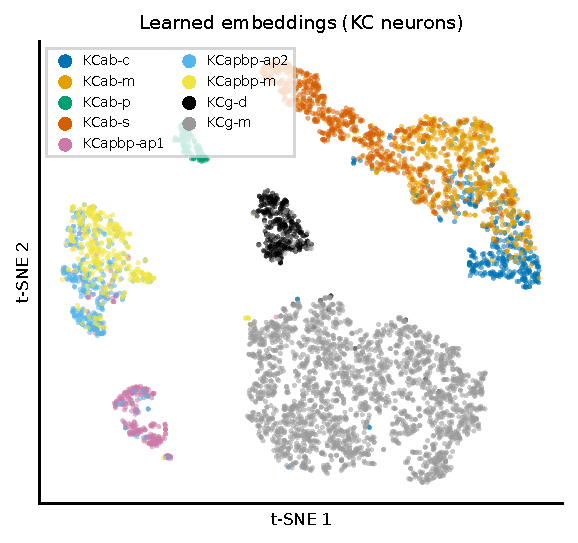
\includegraphics[width=0.48\linewidth]{figures/Fig10_GNN_tsne.pdf}%
\hfill
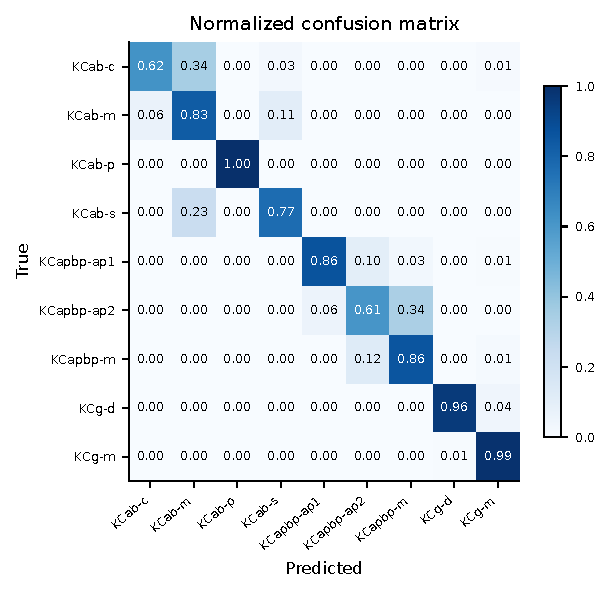
\includegraphics[width=0.48\linewidth]{figures/Fig10_GNN_confusion.pdf}
\vspace{0.3em}
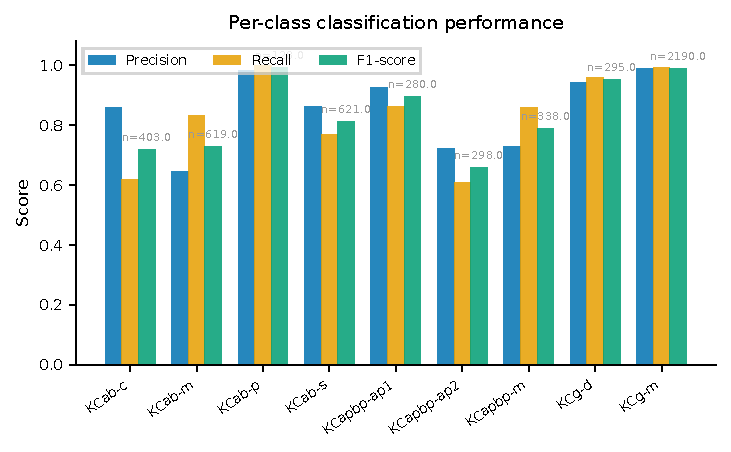
\includegraphics[width=\linewidth]{figures/Fig10_GNN_per_class.pdf}
\caption{\textbf{Connectivity-graph GNN: detailed classification results.}
\textbf{Top left}: t-SNE of learned 64D GNN embeddings for 5,172 KC neurons (9 types).
\textbf{Top right}: Normalised confusion matrix.
\textbf{Bottom}: Per-class precision, recall, and F1-score.}
\label{fig:gnn_results}
\end{figure}

% ════════════════════════════════════════════════════════════════════════
%  EXTENDED DATA FIGURES — All-NT Validation
% ════════════════════════════════════════════════════════════════════════

\begin{figure}[!ht]
\centering
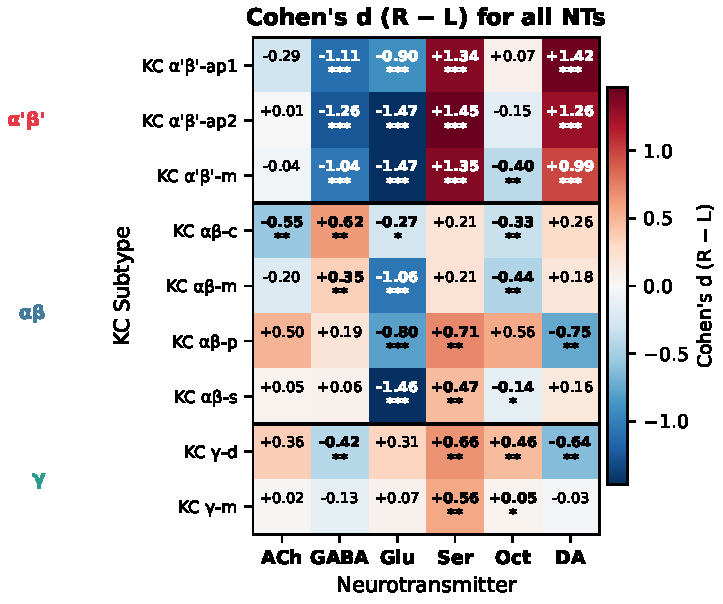
\includegraphics[width=\linewidth]{figures/Fig_ext1_cohens_d_heatmap_all_NT.pdf}
\caption{\textbf{Extended Data Fig.~1: Cohen's $d$ heatmap for all six neurotransmitters across 9 KC types.} Positive values (red) indicate right-enrichment; negative values (blue) indicate left-enrichment. Asterisks denote Bonferroni significance. Horizontal lines separate the three lobe systems ($\alpha'\beta'$, $\alpha\beta$, $\gamma$). Serotonin is right-enriched in 9/9 types; glutamate is left-enriched in 7/9; dopamine is right-enriched in 6/9 with extreme effects in $\alpha'\beta'$ ($d > +1.3$).}
\label{fig:ext_heatmap}
\end{figure}

\begin{figure}[!ht]
\centering
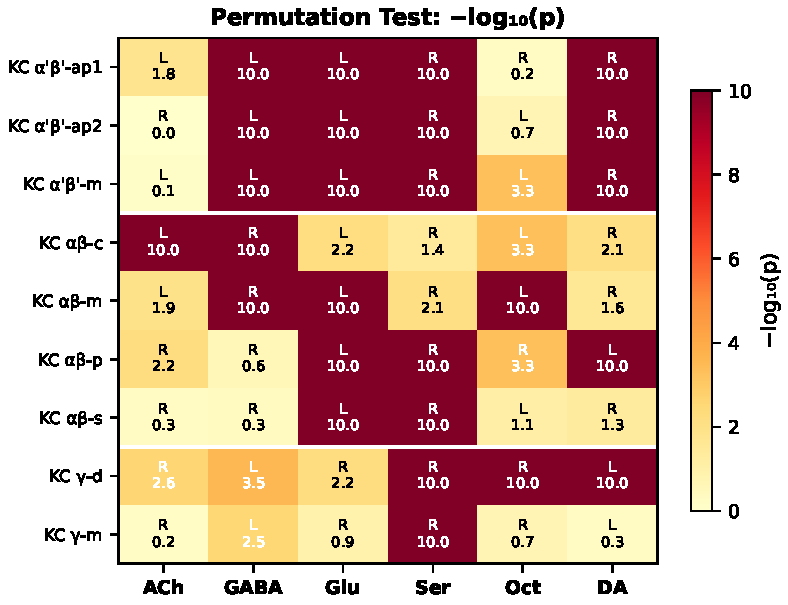
\includegraphics[width=\linewidth]{figures/Fig_ext2_permutation_heatmap.pdf}
\caption{\textbf{Extended Data Fig.~2: GPU permutation test results.} Heatmap shows $-\log_{10}(p)$ from 10,000 label permutations per test. Higher values indicate stronger evidence against the null. Direction of effect (R or L) shown in each cell.}
\label{fig:ext_perm}
\end{figure}

\begin{figure}[!ht]
\centering
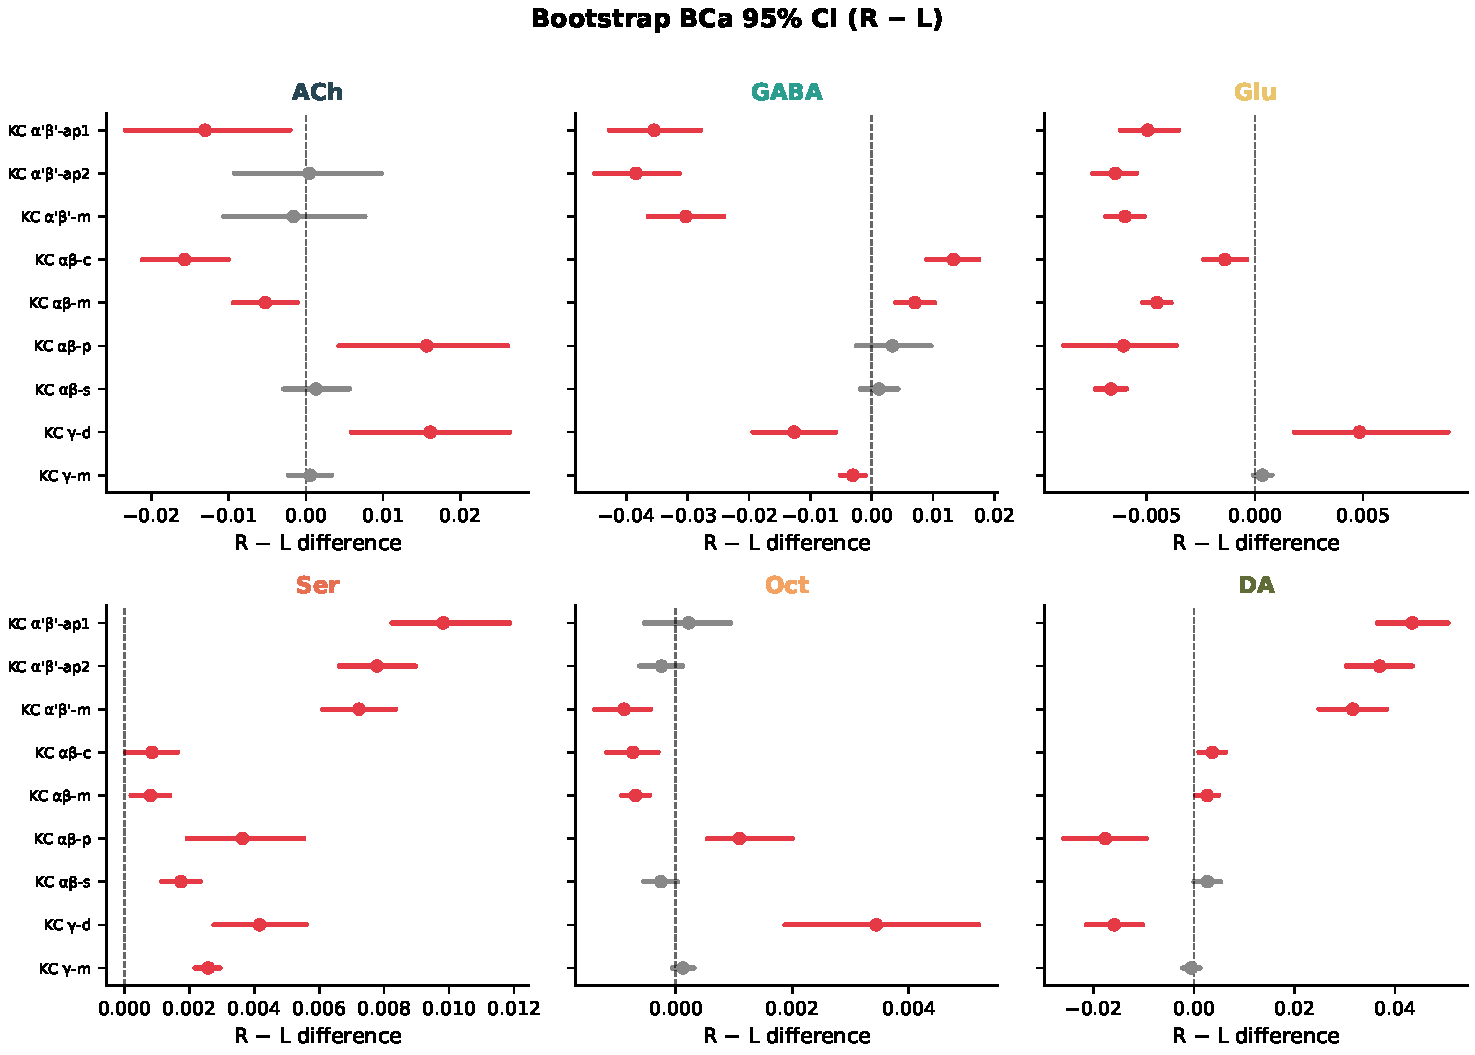
\includegraphics[width=\linewidth]{figures/Fig_ext3_bootstrap_forest.pdf}
\caption{\textbf{Extended Data Fig.~3: Bootstrap BCa 95\% confidence intervals.} Forest plots for each NT showing the R$-$L mean difference and its bootstrap CI for each KC type. Red intervals exclude zero (significant); grey intervals include zero. Serotonin CIs exclude zero in all 9/9 types.}
\label{fig:ext_forest}
\end{figure}

\begin{figure}[!ht]
\centering
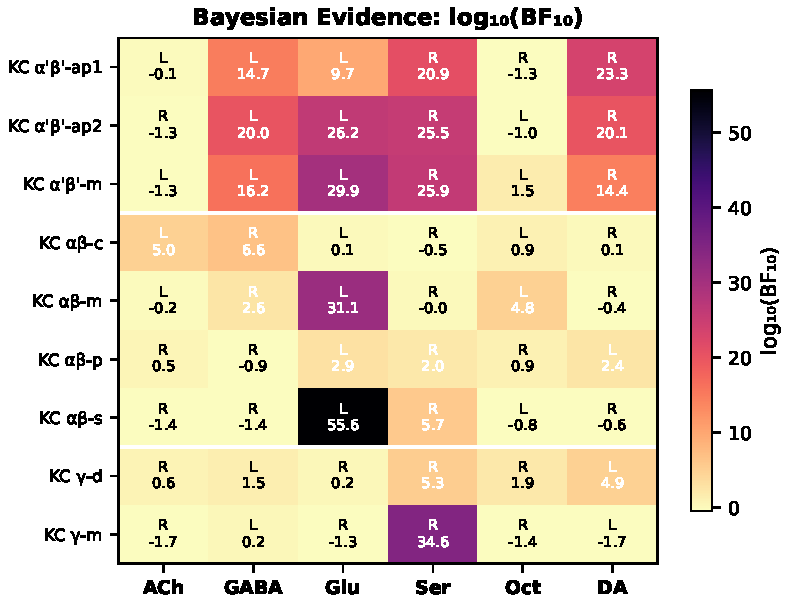
\includegraphics[width=\linewidth]{figures/Fig_ext4_bayesian_bf10.pdf}
\caption{\textbf{Extended Data Fig.~4: Bayesian evidence heatmap.} $\log_{10}(\mathrm{BF}_{10})$ from JZS Bayesian $t$-tests (Rouder et al.\ 2009). Values $> 2$ indicate extreme evidence ($\mathrm{BF}_{10} > 100$). 25/54 tests show extreme Bayesian evidence, with serotonin extreme in 7/9 types.}
\label{fig:ext_bayes}
\end{figure}

\begin{figure}[!ht]
\centering
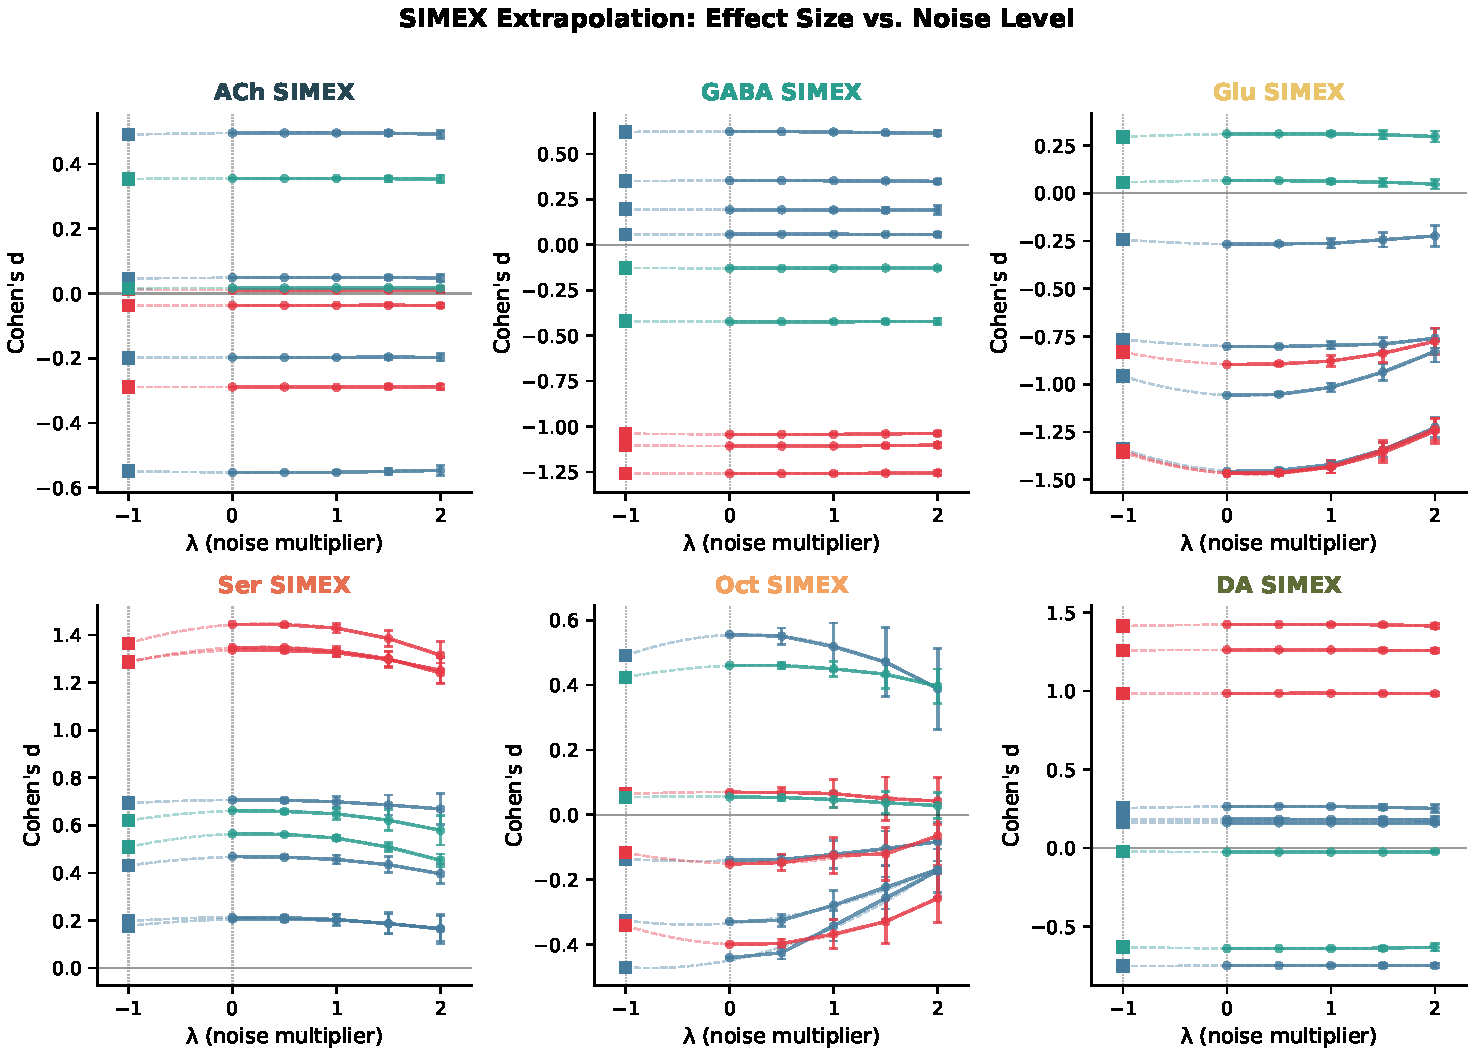
\includegraphics[width=\linewidth]{figures/Fig_ext5_simex_curves.pdf}
\caption{\textbf{Extended Data Fig.~5: SIMEX extrapolation.} Cohen's $d$ as a function of noise multiplier $\lambda$ for each NT. Each line represents one KC type. Squares at $\lambda = -1$ show the quadratic extrapolation to zero measurement error. All serotonin effects (9/9 types) maintain their R$>$L direction after SIMEX extrapolation.}
\label{fig:ext_simex}
\end{figure}

\begin{figure}[!ht]
\centering
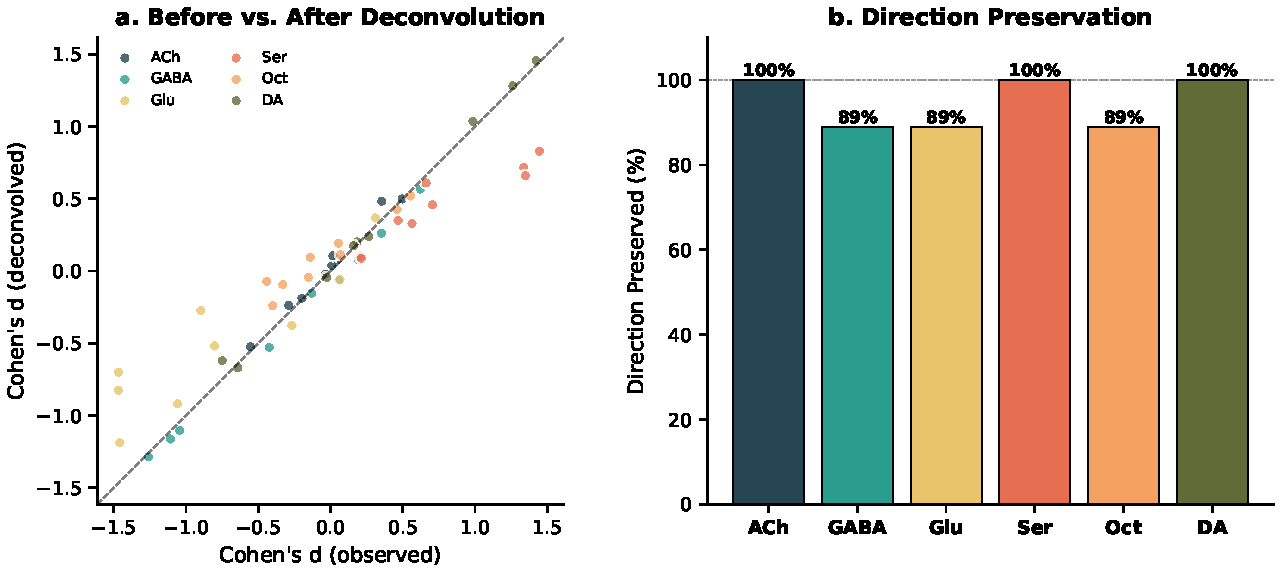
\includegraphics[width=\linewidth]{figures/Fig_ext6_deconvolution.pdf}
\caption{\textbf{Extended Data Fig.~6: Gold's iterative deconvolution.} \textbf{a}, Scatter plot comparing Cohen's $d$ before and after confusion-matrix deconvolution. Points near the identity line indicate robust effects. \textbf{b}, Percentage of effects that preserved their direction after deconvolution, by NT.}
\label{fig:ext_deconv}
\end{figure}

\begin{figure}[!ht]
\centering
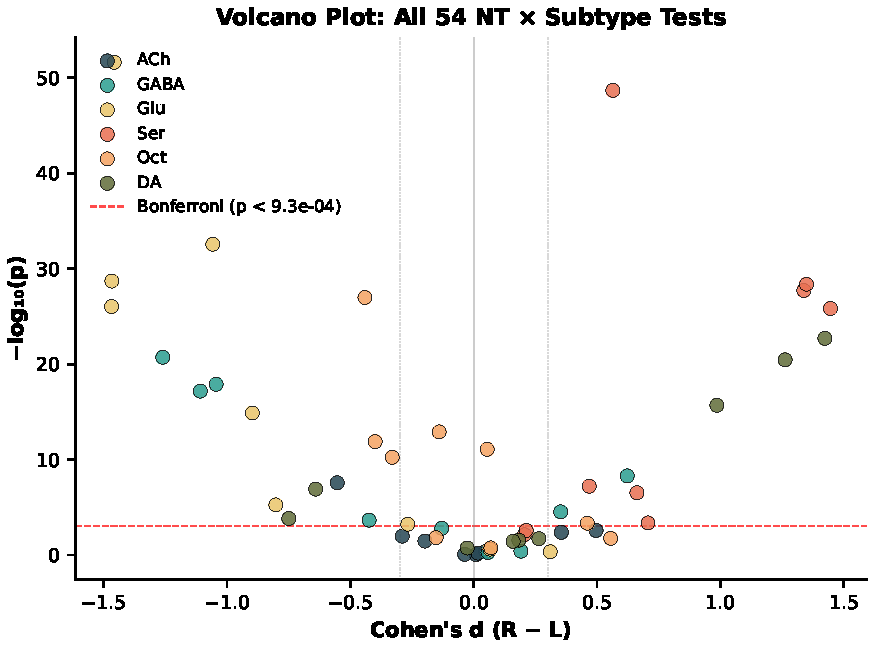
\includegraphics[width=\linewidth]{figures/Fig_ext7_volcano_all_NT.pdf}
\caption{\textbf{Extended Data Fig.~7: Volcano plot of all 54 NT $\times$ type tests.} Serotonin (orange) and dopamine (green) cluster in the R$>$L quadrant; glutamate (yellow) and GABA (teal) cluster in L$>$R, revealing coordinated neuromodulatory lateralization. Dashed red line: Bonferroni threshold.}
\label{fig:ext_volcano}
\end{figure}

\begin{figure}[!ht]
\centering
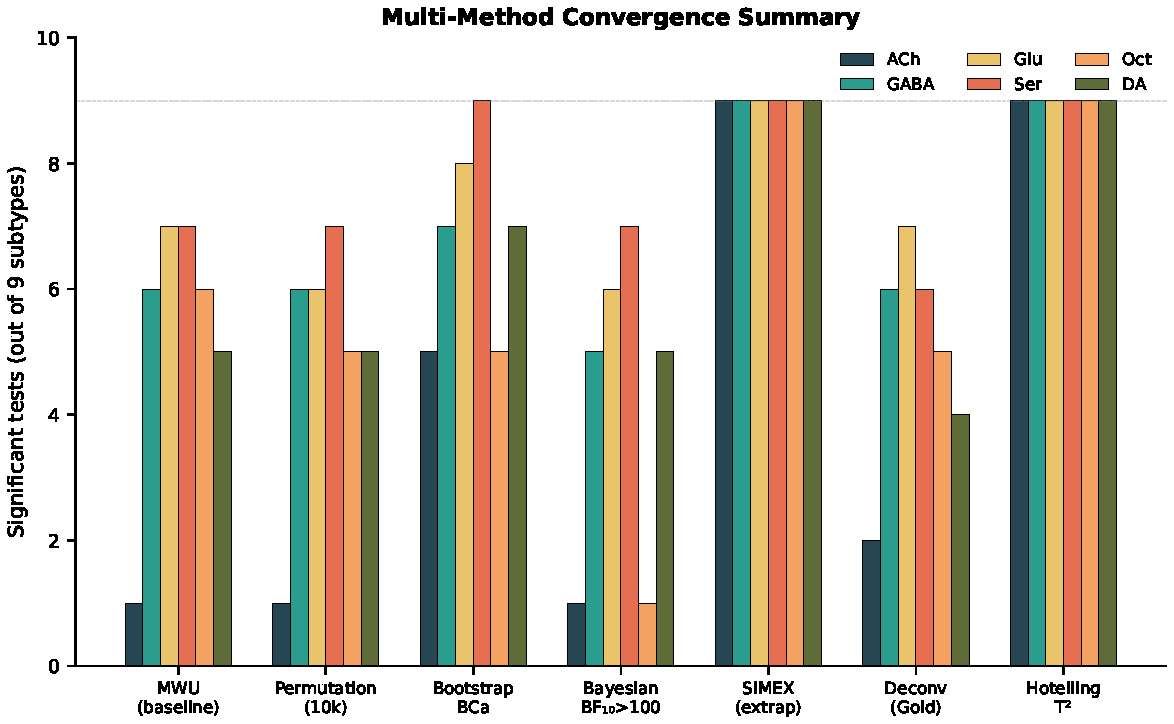
\includegraphics[width=\linewidth]{figures/Fig_ext8_convergence_summary.pdf}
\caption{\textbf{Extended Data Fig.~8: Multi-method convergence.} Number of significant tests (out of 9 types) for each NT across seven independent statistical methods. The consistency of serotonin significance across all methods provides the strongest evidence for lateralization.}
\label{fig:ext_convergence}
\end{figure}

\begin{thebibliography}{99}
\bibitem{scheffer2020hemibrain} Scheffer, L.K. et al. A connectome and analysis of the adult \textit{Drosophila} central brain. \textit{eLife} \textbf{9}, e57443 (2020).
\bibitem{dorkenwald2024flywire} Dorkenwald, S. et al. Neuronal wiring diagram of an adult brain. \textit{Nature} \textbf{634}, 124--138 (2024).
\bibitem{schlegel2024flywire} Schlegel, P. et al. Whole-brain annotation and multi-connectome cell typing of \textit{Drosophila}. \textit{Nature} \textbf{634}, 139--152 (2024).
\bibitem{schwartzman2026ntac} Schwartzman, G. et al. NTAC: Neuronal type assignment from connectivity. \textit{Nature Communications} \textbf{17}, 1284 (2026).
\bibitem{eckstein2020neurotransmitter} Eckstein, N. et al. Neurotransmitter classification from electron microscopy images at synaptic sites in \textit{Drosophila melanogaster}. \textit{Cell} \textbf{187}, 2574--2594 (2024).
\bibitem{costa2016nblast} Costa, M. et al. NBLAST: Rapid, sensitive comparison of neuronal structure and construction of neuron family databases. \textit{Neuron} \textbf{91}, 293--311 (2016).
\bibitem{li2023gnn_neuro} Li, S. et al. Graph neural network-based neuron morphology classification. \textit{Neuroinformatics} (2023).
\bibitem{li2020kc_types} Li, F. et al. The connectome of the adult \textit{Drosophila} mushroom body provides insights into function. \textit{eLife} \textbf{9}, e62576 (2020).
\bibitem{aso2014mushroom} Aso, Y. et al. The neuronal architecture of the mushroom body provides a logic for associative learning. \textit{eLife} \textbf{3}, e04577 (2014).
\bibitem{modi2020dopamine_kc} Modi, M.N. et al. The \textit{Drosophila} mushroom body: from architecture to algorithm in a learning circuit. \textit{Annu.\ Rev.\ Neurosci.} \textbf{43}, 465--484 (2020).
\bibitem{karolis2019lateralisation} Karolis, V.R. et al. The architecture of functional lateralisation and its relationship to callosal connectivity in the human brain. \textit{Nat.\ Commun.} \textbf{10}, 1417 (2019).
\bibitem{wan2024microstructural} Wan, B. et al. Heritability and cross-species comparisons of human cortical functional organization asymmetry. \textit{eLife} \textbf{11}, e77215 (2022).
\bibitem{pascual2004lateralized} Pascual, A. et al. Localization of long-term memory within the \textit{Drosophila} mushroom body. \textit{Science} \textbf{304}, 1024--1027 (2004).
\bibitem{pedigo2023bilateral_elife} Pedigo, B.D. et al. Bisected graph matching improves automated pairing of bilaterally homologous neurons from connectomes. \textit{eLife} \textbf{12}, e80664 (2023).
\bibitem{winding2023larva} Winding, M. et al. The connectome of an insect brain. \textit{Science} \textbf{379}, eadd9330 (2023).
\bibitem{krashes2007sequential} Krashes, M.J. et al. Sequential use of mushroom body neuron subsets during \textit{Drosophila} odor memory processing. \textit{Neuron} \textbf{53}, 103--115 (2007).
\bibitem{keene2006dpm} Keene, A.C. et al. \textit{Drosophila} dorsal paired medial neurons provide a general mechanism for memory consolidation. \textit{Curr.\ Biol.} \textbf{16}, 1524--1530 (2006).
\bibitem{waddell2013serotonin} Waddell, S. Reinforcement signalling in \textit{Drosophila}; dopamine does it all after all. \textit{Curr.\ Opin.\ Neurobiol.} \textbf{23}, 324--329 (2013).
\bibitem{microns2021cortical} MICrONS Consortium et al. Functional connectomics spanning multiple areas of mouse visual cortex. \textit{bioRxiv} (2021).
\bibitem{takemura2013visual} Takemura, S. et al. A visual motion detection circuit suggested by \textit{Drosophila} connectomics. \textit{Nature} \textbf{500}, 175--181 (2013).
\bibitem{shinomiya2019tm} Shinomiya, K. et al. Comparisons between the ON- and OFF-edge motion pathways in the \textit{Drosophila} brain. \textit{eLife} \textbf{8}, e42344 (2019).
\bibitem{linneweber2020asymmetry} Linneweber, G.A. et al. A neurodevelopmental origin of behavioral individuality in the \textit{Drosophila} visual system. \textit{Science} \textbf{367}, 1112--1119 (2020).
\bibitem{thakoor2022bgrl} Thakoor, S. et al. Large-scale representation learning on graphs via bootstrapping. \textit{ICLR} (2022).
\bibitem{rouder2009bayesian} Rouder, J.N. et al. Bayesian $t$ tests for accepting and rejecting the null hypothesis. \textit{Psychon.\ Bull.\ Rev.} \textbf{16}, 225--237 (2009).
\bibitem{cook2006simex} Cook, J.R. \& Stefanski, L.A. Simulation-extrapolation estimation in parametric measurement error models. \textit{J.\ Am.\ Stat.\ Assoc.} \textbf{89}, 1314--1328 (1994).
\end{thebibliography}

\end{document}
